\documentclass[8pt]{extarticle}
\usepackage[utf8]{inputenc}
\usepackage[T1]{fontenc}
\usepackage{amsmath, amssymb}
\usepackage{graphicx}
\usepackage{listings}
\usepackage{xcolor}
\usepackage[a4paper, landscape, left=1cm, right=1cm, top=1.5cm, bottom=1cm, headheight=15pt]{geometry}
\usepackage{multicol}
\usepackage{tocloft}
\usepackage[many]{tcolorbox}
\usepackage{fancyhdr}
\pagestyle{fancy}
\fancyhf{}
\fancyhead[L]{\textbf{CSES Problem Set - UNICAMP}}
\fancyhead[R]{\textbf{Página \thepage}}
\renewcommand{\headrulewidth}{0.4pt}
\renewcommand{\footrulewidth}{0pt}
\fancypagestyle{plain}{
    \fancyhf{}
    \fancyhead[L]{\textbf{CSES Problem Set - UNICAMP}}
    \fancyhead[R]{\textbf{Página \thepage}}
    \renewcommand{\headrulewidth}{0.4pt}
}
\addtolength{\cftsecnumwidth}{0.5em}
\addtolength{\cftsubsecnumwidth}{1.2em}
\setlength{\columnseprule}{0.4pt}
\setlength{\columnsep}{25pt}

% --- CONFIGURAÇÃO DA CAIXA DO ENUNCIADO ---
\newtcolorbox{caixaenunciado}{
    colback=gray!5, % Fundo cinza bem claro e elegante
    colframe=gray!40, % Borda cinza um pouco mais escura
    arc=2pt, % Cantos levemente arredondados
    boxrule=0.5pt, % Espessura da borda
    left=4pt, right=4pt, top=4pt, bottom=4pt,
    breakable, % Essencial: permite que a caixa se divida em colunas
    before skip=0.2cm, after skip=0.2cm
}

\lstset{
    language=C++,
    basicstyle=\ttfamily\footnotesize,
    keywordstyle=\color{blue},
    commentstyle=\color{green!50!black},
    stringstyle=\color{red},
    numbers=left,
    numberstyle=\tiny,
    numbersep=5pt,
    stepnumber=1,
    xleftmargin=2.0em,
    framexleftmargin=2.0em,
    breaklines=true,
    tabsize=4,
    extendedchars=true,
    literate={á}{{\'a}}1 {ã}{{\~a}}1 {é}{{\'e}}1 {í}{{\'i}}1 {ó}{{\'o}}1 {õ}{{\~o}}1 {ú}{{\'u}}1 {ç}{{\c{c}}}1 {Á}{{\'A}}1 {É}{{\'E}}1 {Í}{{\'I}}1 {Ó}{{\'O}}1 {Ú}{{\'U}}1 {Ç}{{\c{C}}}1 {Ã}{{\~A}}1 {Õ}{{\~O}}1
}

\begin{document}
\begin{titlepage}
    \centering
    \vspace*{1.5cm}
    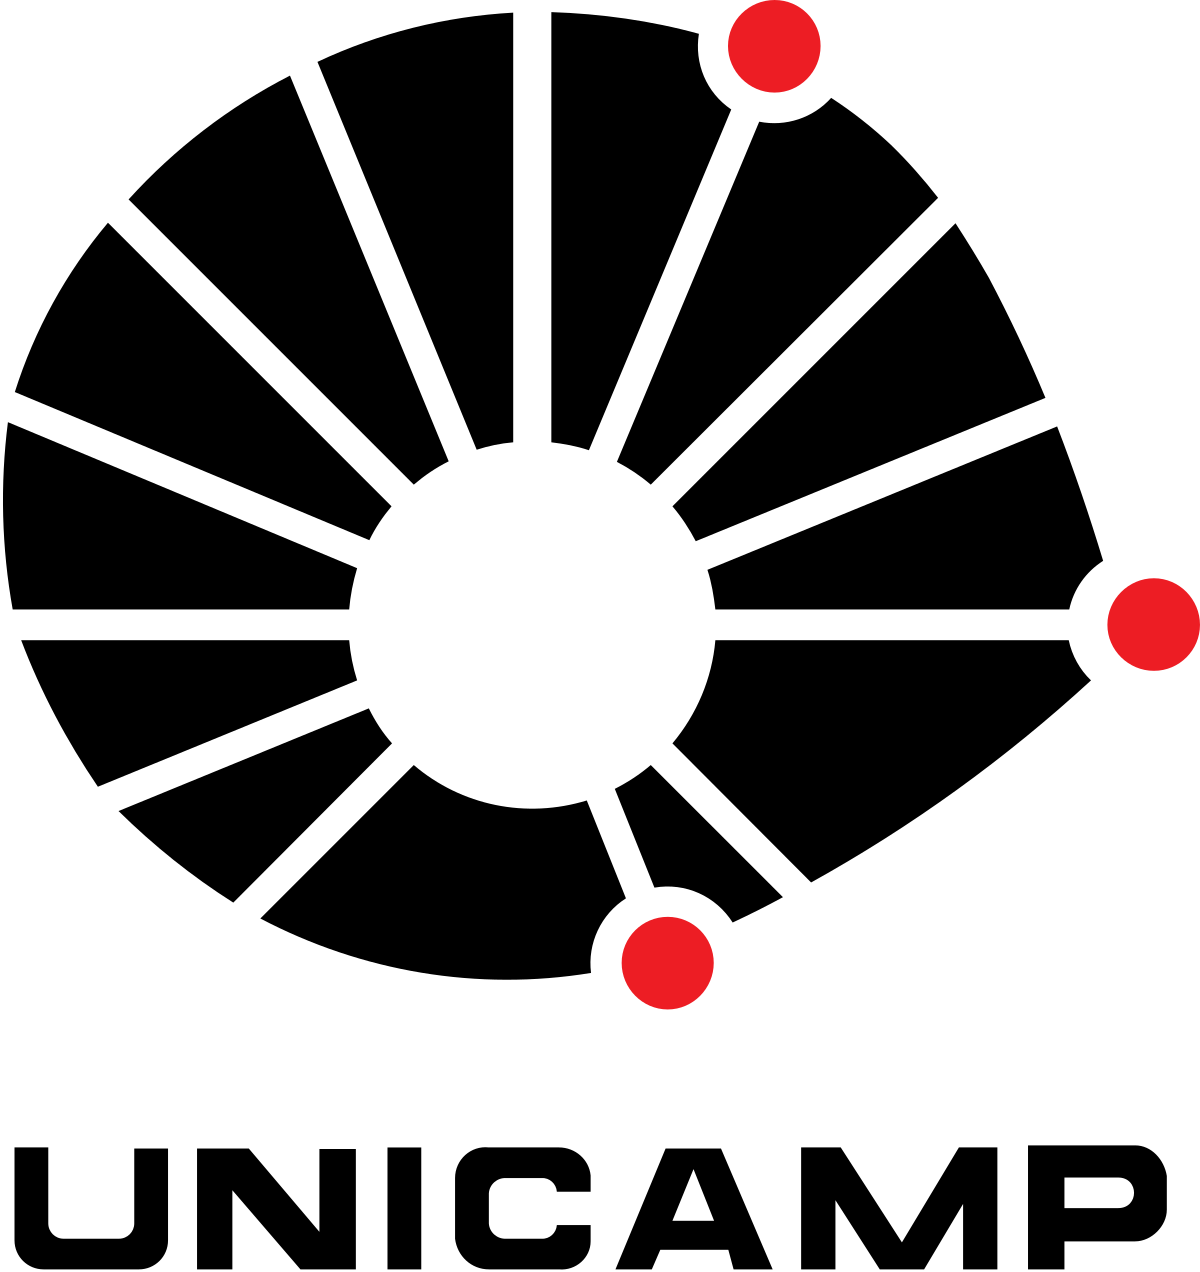
\includegraphics[width=4.5cm]{unicamp.png} \par
    \vspace{0.4cm}
    {\fontsize{16}{20}\selectfont Universidade Estadual de Campinas \par}
    \vspace{1.2cm}
    {\fontsize{42}{50}\selectfont Enemy Leo used Appeal! It's \par}
    \vspace{0.2cm}
    {\fontsize{42}{50}\selectfont super effective! Pikachu fainted! \par}
    \vspace{1.5cm}
    {\fontsize{20}{24}\selectfont \textbf{CSES Problem Set} \par}
    \vspace{1cm}
    {\fontsize{14}{18}\selectfont Pedro Assunção, Pedro Mesquita, Yvens Porto \par}
    \vfill
    {\fontsize{12}{14}\selectfont 2026-08-18 \par}
\end{titlepage}
\begin{multicols*}{3}
\tableofcontents
\end{multicols*}
\pagebreak
\begin{multicols*}{3}

\section{Introductory Problems}

\subsection{Apple Division}
\begin{caixaenunciado}
There are $n$ apples with known weights. Your task is to divide the apples into two groups so that the difference between the weights of the groups is minimal.

\vspace{0.3cm}\noindent\textbf{Input}

The first input line has an integer $n$: the number of apples.
The next line has $n$ integers $p_1,p_2,\dots,p_n$: the weight of each apple.

\vspace{0.3cm}\noindent\textbf{Output}

Print one integer: the minimum difference between the weights of the groups.

\vspace{0.3cm}\noindent\textbf{Constraints}

\textbullet\ $1 \le n \le 20$
\textbullet\ $1 \le p_i \le 10^9$
\end{caixaenunciado}
\vspace{0.3cm}
\noindent\textbf{Código-fonte:}
\lstinputlisting{IntroductoryProblems/AppleDivision.cpp}

\subsection{Bit Strings}
\begin{caixaenunciado}
Your task is to calculate the number of bit strings of length $n$.
For example, if $n=3$, the correct answer is $8$, because the possible bit strings are 000, 001, 010, 011, 100, 101, 110, and 111.

\vspace{0.3cm}\noindent\textbf{Input}

The only input line has an integer $n$.

\vspace{0.3cm}\noindent\textbf{Output}

Print the result modulo $10^9+7$.

\vspace{0.3cm}\noindent\textbf{Constraints}

\textbullet\ $1 \le n \le 10^6$
\end{caixaenunciado}
\vspace{0.3cm}
\noindent\textbf{Código-fonte:}
\lstinputlisting{IntroductoryProblems/BitStrings.cpp}

\subsection{Chessboardand Queens}
\begin{caixaenunciado}
Your task is to place eight queens on a chessboard so that no two queens are attacking each other. As an additional challenge, each square is either free or reserved, and you can only place queens on the free squares. However, the reserved squares do not prevent queens from attacking each other.
How many possible ways are there to place the queens?

\vspace{0.3cm}\noindent\textbf{Input}

The input has eight lines, and each of them has eight characters. Each square is either free (.) or reserved (*).

\vspace{0.3cm}\noindent\textbf{Output}

Print one integer: the number of ways you can place the queens.
\end{caixaenunciado}
\vspace{0.3cm}
\noindent\textbf{Código-fonte:}
\lstinputlisting{IntroductoryProblems/ChessboardandQueens.cpp}

\subsection{Coin Piles}
\begin{caixaenunciado}
You have two coin piles containing $a$ and $b$ coins. On each move, you can either remove one coin from the left pile and two coins from the right pile, or two coins from the left pile and one coin from the right pile.
Your task is to efficiently find out if you can empty both the piles.

\vspace{0.3cm}\noindent\textbf{Input}

The first input line has an integer $t$: the number of tests.
After this, there are $t$ lines, each of which has two integers $a$ and $b$: the numbers of coins in the piles.

\vspace{0.3cm}\noindent\textbf{Output}

For each test, print "YES" if you can empty the piles and "NO" otherwise.

\vspace{0.3cm}\noindent\textbf{Constraints}

\textbullet\ $1 \le t \le 10^5$
\textbullet\ $0 \le a, b \le 10^9$
\end{caixaenunciado}
\vspace{0.3cm}
\noindent\textbf{Código-fonte:}
\lstinputlisting{IntroductoryProblems/CoinPiles.cpp}

\subsection{Creating Strings}
\begin{caixaenunciado}
Given a string, your task is to generate all different strings that can be created using its characters.

\vspace{0.3cm}\noindent\textbf{Input}

The only input line has a string of length $n$. Each character is between a–z.

\vspace{0.3cm}\noindent\textbf{Output}

First print an integer $k$: the number of strings. Then print $k$ lines: the strings in alphabetical order.

\vspace{0.3cm}\noindent\textbf{Constraints}

\textbullet\ $1 \le n \le 8$
\end{caixaenunciado}
\vspace{0.3cm}
\noindent\textbf{Código-fonte:}
\lstinputlisting{IntroductoryProblems/CreatingStrings.cpp}

\subsection{Digit Queries}
\begin{caixaenunciado}
Consider an infinite string that consists of all positive integers in increasing order:
12345678910111213141516171819202122232425...
Your task is to process $q$ queries of the form: what is the digit at position $k$ in the string?

\vspace{0.3cm}\noindent\textbf{Input}

The first input line has an integer $q$: the number of queries.
After this, there are $q$ lines that describe the queries. Each line has an integer $k$: a $1$-indexed position in the string.

\vspace{0.3cm}\noindent\textbf{Output}

For each query, print the corresponding digit.

\vspace{0.3cm}\noindent\textbf{Constraints}

\textbullet\ $1 \le q \le 1000$
\textbullet\ $1 \le k \le 10^{18}$
\end{caixaenunciado}
\vspace{0.3cm}
\noindent\textbf{Código-fonte:}
\lstinputlisting{IntroductoryProblems/DigitQueries.cpp}

\subsection{Gray Code}
\begin{caixaenunciado}
A Gray code is a list of all $2^n$ bit strings of length $n$, where any two successive strings differ in exactly one bit (i.e., their Hamming distance is one).
Your task is to create a Gray code for a given length $n$.

\vspace{0.3cm}\noindent\textbf{Input}

The only input line has an integer $n$.

\vspace{0.3cm}\noindent\textbf{Output}

Print $2^n$ lines that describe the Gray code. You can print any valid solution.

\vspace{0.3cm}\noindent\textbf{Constraints}

\textbullet\ $1 \le n \le 16$
\end{caixaenunciado}
\vspace{0.3cm}
\noindent\textbf{Código-fonte:}
\lstinputlisting{IntroductoryProblems/GrayCode.cpp}

\subsection{Grid Coloring I}
\begin{caixaenunciado}
\input{Enunciados/IntroductoryProblems/GridColoringI.tex}
\end{caixaenunciado}
\vspace{0.3cm}
\noindent\textbf{Código-fonte:}
\lstinputlisting{IntroductoryProblems/GridColoringI.cpp}

\subsection{Grid Path Description}
\begin{caixaenunciado}
\input{Enunciados/IntroductoryProblems/GridPathDescription.tex}
\end{caixaenunciado}
\vspace{0.3cm}
\noindent\textbf{Código-fonte:}
\lstinputlisting{IntroductoryProblems/GridPathDescription.cpp}

\subsection{Increasing Array}
\begin{caixaenunciado}
You are given an array of $n$ integers. You want to modify the array so that it is increasing, i.e., every element is at least as large as the previous element.
On each move, you may increase the value of any element by one. What is the minimum number of moves required?

\vspace{0.3cm}\noindent\textbf{Input}

The first input line contains an integer $n$: the size of the array.
Then, the second line contains $n$ integers $x_1,x_2,\ldots,x_n$: the contents of the array.

\vspace{0.3cm}\noindent\textbf{Output}

Print the minimum number of moves.

\vspace{0.3cm}\noindent\textbf{Constraints}

\textbullet\ $1 \le n \le 2 \cdot 10^5$
\textbullet\ $1 \le x_i \le 10^9$
\end{caixaenunciado}
\vspace{0.3cm}
\noindent\textbf{Código-fonte:}
\lstinputlisting{IntroductoryProblems/IncreasingArray.cpp}

\subsection{Knight Moves Grid}
\begin{caixaenunciado}
There is a knight on an $n \times n$ chessboard. For each square, print the minimum number of moves the knight needs to do to reach the top-left corner.

\vspace{0.3cm}\noindent\textbf{Input}

The only line has an integer $n$.

\vspace{0.3cm}\noindent\textbf{Output}

Print the number of moves for each square.

\vspace{0.3cm}\noindent\textbf{Constraints}

\textbullet\ $4 \le n \le 1000$
\end{caixaenunciado}
\vspace{0.3cm}
\noindent\textbf{Código-fonte:}
\lstinputlisting{IntroductoryProblems/KnightMovesGrid.cpp}

\subsection{Mex Grid Construction}
\begin{caixaenunciado}
Your task is to construct an $n \times n$ grid where each square has the smallest nonnegative integer that does not appear to the left on the same row or above on the same column.

\vspace{0.3cm}\noindent\textbf{Input}

The only line has an integer $n$.

\vspace{0.3cm}\noindent\textbf{Output}

Print the grid according to the example.

\vspace{0.3cm}\noindent\textbf{Constraints}

\textbullet\ $1 \le n \le 100$
\end{caixaenunciado}
\vspace{0.3cm}
\noindent\textbf{Código-fonte:}
\lstinputlisting{IntroductoryProblems/MexGridConstruction.cpp}

\subsection{Missing Number}
\begin{caixaenunciado}
You are given all numbers between $1,2,\ldots,n$ except one. Your task is to find the missing number.

\vspace{0.3cm}\noindent\textbf{Input}

The first input line contains an integer $n$.
The second line contains $n-1$ numbers. Each number is distinct and between $1$ and $n$ (inclusive).

\vspace{0.3cm}\noindent\textbf{Output}

Print the missing number.

\vspace{0.3cm}\noindent\textbf{Constraints}

\textbullet\ $2 \le n \le 2 \cdot 10^5$
\end{caixaenunciado}
\vspace{0.3cm}
\noindent\textbf{Código-fonte:}
\lstinputlisting{IntroductoryProblems/MissingNumber.cpp}

\subsection{Number Spiral}
\begin{caixaenunciado}
A number spiral is an infinite grid whose upper-left square has number 1. Here are the first five layers of the spiral:

Your task is to find out the number in row $y$ and column $x$.

\vspace{0.3cm}\noindent\textbf{Input}

The first input line contains an integer $t$: the number of tests.
After this, there are $t$ lines, each containing integers $y$ and $x$.

\vspace{0.3cm}\noindent\textbf{Output}

For each test, print the number in row $y$ and column $x$.

\vspace{0.3cm}\noindent\textbf{Constraints}

\textbullet\ $1 \le t \le 10^5$
\textbullet\ $1 \le y,x \le 10^9$
\end{caixaenunciado}
\vspace{0.3cm}
\noindent\textbf{Código-fonte:}
\lstinputlisting{IntroductoryProblems/NumberSpiral.cpp}

\subsection{Palindrome Reorder}
\begin{caixaenunciado}
Given a string, your task is to reorder its letters in such a way that it becomes a palindrome (i.e., it reads the same forwards and backwards).

\vspace{0.3cm}\noindent\textbf{Input}

The only input line has a string of length $n$ consisting of characters A–Z.

\vspace{0.3cm}\noindent\textbf{Output}

Print a palindrome consisting of the characters of the original string. You may print any valid solution. If there are no solutions, print "NO SOLUTION".

\vspace{0.3cm}\noindent\textbf{Constraints}

\textbullet\ $1 \le n \le 10^6$
\end{caixaenunciado}
\vspace{0.3cm}
\noindent\textbf{Código-fonte:}
\lstinputlisting{IntroductoryProblems/PalindromeReorder.cpp}

\subsection{Permutations}
\begin{caixaenunciado}
A permutation of integers $1,2,\ldots,n$ is called beautiful if there are no adjacent elements whose difference is $1$.
Given $n$, construct a beautiful permutation if such a permutation exists.

\vspace{0.3cm}\noindent\textbf{Input}

The only input line contains an integer $n$.

\vspace{0.3cm}\noindent\textbf{Output}

Print a beautiful permutation of integers $1,2,\ldots,n$. If there are several solutions, you may print any of them. If there are no solutions, print "NO SOLUTION".

\vspace{0.3cm}\noindent\textbf{Constraints}

\textbullet\ $1 \le n \le 10^6$
\end{caixaenunciado}
\vspace{0.3cm}
\noindent\textbf{Código-fonte:}
\lstinputlisting{IntroductoryProblems/Permutations.cpp}

\subsection{Raab Game I}
\begin{caixaenunciado}
Consider a two player game where each player has $n$ cards numbered $1,2,\dots,n$. On each turn both players place one of their cards on the table. The player who placed the higher card gets one point. If the cards are equal, neither player gets a point. The game continues until all cards have been played.
You are given the number of cards $n$ and the players' scores at the end of the game, $a$ and $b$. Your task is to give an example of how the game could have played out.

\vspace{0.3cm}\noindent\textbf{Input}

The first line contains one integer $t$: the number of tests.
Then there are $t$ lines, each with three integers $n$, $a$ and $b$.

\vspace{0.3cm}\noindent\textbf{Output}

For each test case print YES if there is a game with the given outcome and NO otherwise.
If the answer is YES, print an example of one possible game. Print two lines representing the order in which the players place their cards. You can give any valid example.

\vspace{0.3cm}\noindent\textbf{Constraints}

\textbullet\ $1 \le t \le 1000$
\textbullet\ $1 \le n \le 100$
\textbullet\ $0 \le a,b \le n$
\end{caixaenunciado}
\vspace{0.3cm}
\noindent\textbf{Código-fonte:}
\lstinputlisting{IntroductoryProblems/RaabGameI.cpp}

\subsection{Repetitions}
\begin{caixaenunciado}
\input{Enunciados/IntroductoryProblems/Repetitions.tex}
\end{caixaenunciado}
\vspace{0.3cm}
\noindent\textbf{Código-fonte:}
\lstinputlisting{IntroductoryProblems/Repetitions.cpp}

\subsection{String Reorder}
\begin{caixaenunciado}
Your task is to reorder the characters of a string so that no two adjacent characters are the same. What is the lexicographically minimal such string?

\vspace{0.3cm}\noindent\textbf{Input}

The only line has a string of length $n$ consisting of characters A–Z.

\vspace{0.3cm}\noindent\textbf{Output}

Print the lexicographically minimal reordered string where no two adjacent characters are the same. If it is not possible to create such a string, print $-1$.

\vspace{0.3cm}\noindent\textbf{Constraints}

\textbullet\ $1 \le n \le 10^6$
\end{caixaenunciado}
\vspace{0.3cm}
\noindent\textbf{Código-fonte:}
\lstinputlisting{IntroductoryProblems/StringReorder.cpp}

\subsection{Towerof Hanoi}
\begin{caixaenunciado}
The Tower of Hanoi game consists of three stacks (left, middle and right) and $n$ round disks of different sizes. Initially, the left stack has all the disks, in increasing order of size from top to bottom.
The goal is to move all the disks to the right stack using the middle stack. On each move you can move the uppermost disk from a stack to another stack. In addition, it is not allowed to place a larger disk on a smaller disk.
Your task is to find a solution that minimizes the number of moves.

\vspace{0.3cm}\noindent\textbf{Input}

The only input line has an integer $n$: the number of disks.

\vspace{0.3cm}\noindent\textbf{Output}

First print an integer $k$: the minimum number of moves.
After this, print $k$ lines that describe the moves. Each line has two integers $a$ and $b$: you move a disk from stack $a$ to stack $b$.

\vspace{0.3cm}\noindent\textbf{Constraints}

\textbullet\ $1 \le n \le 16$
\end{caixaenunciado}
\vspace{0.3cm}
\noindent\textbf{Código-fonte:}
\lstinputlisting{IntroductoryProblems/TowerofHanoi.cpp}

\subsection{Trailing Zeros}
\begin{caixaenunciado}
Your task is to calculate the number of trailing zeros in the factorial $n!$.
For example, $20!=2432902008176640000$ and it has $4$ trailing zeros.

\vspace{0.3cm}\noindent\textbf{Input}

The only input line has an integer $n$.

\vspace{0.3cm}\noindent\textbf{Output}

Print the number of trailing zeros in $n!$.

\vspace{0.3cm}\noindent\textbf{Constraints}

\textbullet\ $1 \le n \le 10^9$
\end{caixaenunciado}
\vspace{0.3cm}
\noindent\textbf{Código-fonte:}
\lstinputlisting{IntroductoryProblems/TrailingZeros.cpp}

\subsection{Two Knights}
\begin{caixaenunciado}
Your task is to count for $k=1,2,\ldots,n$ the number of ways two knights can be placed on a $k \times k$ chessboard so that they do not attack each other.

\vspace{0.3cm}\noindent\textbf{Input}

The only input line contains an integer $n$.

\vspace{0.3cm}\noindent\textbf{Output}

Print $n$ integers: the results.

\vspace{0.3cm}\noindent\textbf{Constraints}

\textbullet\ $1 \le n \le 10000$
\end{caixaenunciado}
\vspace{0.3cm}
\noindent\textbf{Código-fonte:}
\lstinputlisting{IntroductoryProblems/TwoKnights.cpp}

\subsection{Two Sets}
\begin{caixaenunciado}
Your task is to divide the numbers $1,2,\ldots,n$ into two sets of equal sum.

\vspace{0.3cm}\noindent\textbf{Input}

The only input line contains an integer $n$.

\vspace{0.3cm}\noindent\textbf{Output}

Print "YES", if the division is possible, and "NO" otherwise.
After this, if the division is possible, print an example of how to create the sets. First, print the number of elements in the first set followed by the elements themselves in a separate line, and then, print the second set in a similar way.

\vspace{0.3cm}\noindent\textbf{Constraints}

\textbullet\ $1 \le n \le 10^6$
\end{caixaenunciado}
\vspace{0.3cm}
\noindent\textbf{Código-fonte:}
\lstinputlisting{IntroductoryProblems/TwoSets.cpp}

\subsection{Weird Algorithm}
\begin{caixaenunciado}
Consider an algorithm that takes as input a positive integer $n$. If $n$ is even, the algorithm divides it by two, and if $n$ is odd, the algorithm multiplies it by three and adds one. The algorithm repeats this, until $n$ is one. For example, the sequence for $n=3$ is as follows:
$ 3 \rightarrow 10 \rightarrow 5 \rightarrow 16 \rightarrow 8 \rightarrow 4 \rightarrow 2 \rightarrow 1$
Your task is to simulate the execution of the algorithm for a given value of $n$.

\vspace{0.3cm}\noindent\textbf{Input}

The only input line contains an integer $n$.

\vspace{0.3cm}\noindent\textbf{Output}

Print a line that contains all values of $n$ during the algorithm.

\vspace{0.3cm}\noindent\textbf{Constraints}

\textbullet\ $1 \le n \le 10^6$
\end{caixaenunciado}
\vspace{0.3cm}
\noindent\textbf{Código-fonte:}
\lstinputlisting{IntroductoryProblems/WeirdAlgorithm.cpp}
\end{multicols*}
\pagebreak
\begin{multicols*}{3}

\section{Dynamic Programming}

\subsection{Array Description}
\begin{caixaenunciado}
You know that an array has $n$ integers between $1$ and  $m$, and the absolute difference between two adjacent values is at most $1$.
Given a description of the array where some values may be unknown, your task is to count the number of arrays that match the description.

\vspace{0.3cm}\noindent\textbf{Input}

The first input line has two integers $n$ and $m$: the array size and the upper bound for each value.
The next line has $n$ integers $x_1,x_2,\dots,x_n$: the contents of the array. Value $0$ denotes an unknown value.

\vspace{0.3cm}\noindent\textbf{Output}

Print one integer: the number of arrays modulo $10^9+7$.

\vspace{0.3cm}\noindent\textbf{Constraints}

\textbullet\ $1 \le n \le 10^5$
\textbullet\ $1 \le m \le 100$
\textbullet\ $0 \le x_i \le m$
\end{caixaenunciado}
\vspace{0.3cm}
\noindent\textbf{Código-fonte:}
\lstinputlisting{DynamicProgramming/ArrayDescription.cpp}

\subsection{Book Shop}
\begin{caixaenunciado}
You are in a book shop which sells $n$ different books. You know the price and number of pages of each book.
You have decided that the total price of your purchases will be at most $x$. What is the maximum number of pages you can buy? You can buy each book at most once.

\vspace{0.3cm}\noindent\textbf{Input}

The first input line contains two integers $n$ and $x$: the number of books and the maximum total price.
The next line contains $n$ integers $h_1,h_2,\ldots,h_n$: the price of each book.
The last line contains $n$ integers $s_1,s_2,\ldots,s_n$: the number of pages of each book.

\vspace{0.3cm}\noindent\textbf{Output}

Print one integer: the maximum number of pages.

\vspace{0.3cm}\noindent\textbf{Constraints}

\textbullet\ $1 \le n \le 1000$
\textbullet\ $1 \le x \le 10^5$
\textbullet\ $1 \le h_i, s_i \le 1000$
\end{caixaenunciado}
\vspace{0.3cm}
\noindent\textbf{Código-fonte:}
\lstinputlisting{DynamicProgramming/BookShop.cpp}

\subsection{Coin Combinations I}
\begin{caixaenunciado}
\input{Enunciados/DynamicProgramming/CoinCombinationsI.tex}
\end{caixaenunciado}
\vspace{0.3cm}
\noindent\textbf{Código-fonte:}
\lstinputlisting{DynamicProgramming/CoinCombinationsI.cpp}

\subsection{Coin Combinations II}
\begin{caixaenunciado}
Consider a money system consisting of $n$ coins. Each coin has a positive integer value. Your task is to calculate the number of distinct ordered ways you can produce a money sum $x$ using the available coins.
For example, if the coins are $\{2,3,5\}$ and the desired sum is $9$, there are $3$ ways:

\textbullet\ $2+2+5$
\textbullet\ $3+3+3$
\textbullet\ $2+2+2+3$

\vspace{0.3cm}\noindent\textbf{Input}

The first input line has two integers $n$ and $x$: the number of coins and the desired sum of money.
The second line has $n$ distinct integers $c_1,c_2,\dots,c_n$: the value of each coin.

\vspace{0.3cm}\noindent\textbf{Output}

Print one integer: the number of ways modulo $10^9+7$.

\vspace{0.3cm}\noindent\textbf{Constraints}

\textbullet\ $1 \le n \le 100$
\textbullet\ $1 \le x \le 10^6$
\textbullet\ $1 \le c_i \le 10^6$
\end{caixaenunciado}
\vspace{0.3cm}
\noindent\textbf{Código-fonte:}
\lstinputlisting{DynamicProgramming/CoinCombinationsII.cpp}

\subsection{Counting Numbers}
\begin{caixaenunciado}
Your task is to count the number of integers between $a$ and $b$ where no two adjacent digits are the same.

\vspace{0.3cm}\noindent\textbf{Input}

The only input line has two integers $a$ and $b$.

\vspace{0.3cm}\noindent\textbf{Output}

Print one integer: the answer to the problem.

\vspace{0.3cm}\noindent\textbf{Constraints}

\textbullet\ $0 \le a \le b \le 10^{18}$
\end{caixaenunciado}
\vspace{0.3cm}
\noindent\textbf{Código-fonte:}
\lstinputlisting{DynamicProgramming/CountingNumbers.cpp}

\subsection{Counting Tiling}
Enunciado não encontrado no site.
\vspace{0.3cm}
\noindent\textbf{Código-fonte:}
\lstinputlisting{DynamicProgramming/CountingTiling.cpp}

\subsection{Counting Towers}
\begin{caixaenunciado}
Your task is to build a tower whose width is $2$ and height is $n$. You have an unlimited supply of blocks whose width and height are integers.
For example, here are some possible solutions for $n=6$:

Given $n$, how many different towers can you build? Mirrored and rotated towers are counted separately if they look different.

\vspace{0.3cm}\noindent\textbf{Input}

The first input line contains an integer $t$: the number of tests.
After this, there are $t$ lines, and each line contains an integer $n$: the height of the tower.

\vspace{0.3cm}\noindent\textbf{Output}

For each test, print the number of towers modulo $10^9+7$.

\vspace{0.3cm}\noindent\textbf{Constraints}

\textbullet\ $1 \le t \le 100$
\textbullet\ $1 \le n \le 10^6$
\end{caixaenunciado}
\vspace{0.3cm}
\noindent\textbf{Código-fonte:}
\lstinputlisting{DynamicProgramming/CountingTowers.cpp}

\subsection{Dice Combinations}
\begin{caixaenunciado}
Your task is to count the number of ways to construct sum $n$ by throwing a dice one or more times. Each throw produces an outcome between $1$ and  $6$.
For example, if $n=3$, there are $4$ ways:

\textbullet\ $1+1+1$
\textbullet\ $1+2$
\textbullet\ $2+1$
\textbullet\ $3$

\vspace{0.3cm}\noindent\textbf{Input}

The only input line has an integer $n$.

\vspace{0.3cm}\noindent\textbf{Output}

Print the number of ways modulo $10^9+7$.

\vspace{0.3cm}\noindent\textbf{Constraints}

\textbullet\ $1 \le n \le 10^6$
\end{caixaenunciado}
\vspace{0.3cm}
\noindent\textbf{Código-fonte:}
\lstinputlisting{DynamicProgramming/DiceCombinations.cpp}

\subsection{Edit Distance}
\begin{caixaenunciado}
The edit distance between two strings is the minimum number of operations required to transform one string into the other.
The allowed operations are:

\textbullet\ Add one character to the string.
\textbullet\ Remove one character from the string.
\textbullet\ Replace one character in the string.

For example, the edit distance between LOVE and MOVIE is 2, because you can first replace L with M, and then add I.
Your task is to calculate the edit distance between two strings.

\vspace{0.3cm}\noindent\textbf{Input}

The first input line has a string that contains $n$ characters between A–Z.
The second input line has a string that contains $m$ characters between A–Z.

\vspace{0.3cm}\noindent\textbf{Output}

Print one integer: the edit distance between the strings.

\vspace{0.3cm}\noindent\textbf{Constraints}

\textbullet\ $1 \le n,m \le 5000$
\end{caixaenunciado}
\vspace{0.3cm}
\noindent\textbf{Código-fonte:}
\lstinputlisting{DynamicProgramming/EditDistance.cpp}

\subsection{Elevator Rides}
\begin{caixaenunciado}
There are $n$ people who want to get to the top of a building which has only one elevator. You know the weight of each person and the maximum allowed weight in the elevator. What is the minimum number of elevator rides?

\vspace{0.3cm}\noindent\textbf{Input}

The first input line has two integers $n$ and $x$: the number of people and the maximum allowed weight in the elevator.
The second line has $n$ integers $w_1,w_2,\dots,w_n$: the weight of each person.

\vspace{0.3cm}\noindent\textbf{Output}

Print one integer: the minimum number of rides.

\vspace{0.3cm}\noindent\textbf{Constraints}

\textbullet\ $1 \le n \le 20$
\textbullet\ $1 \le x \le 10^9$
\textbullet\ $1 \le w_i \le x$
\end{caixaenunciado}
\vspace{0.3cm}
\noindent\textbf{Código-fonte:}
\lstinputlisting{DynamicProgramming/ElevatorRides.cpp}

\subsection{Grid Paths I}
\begin{caixaenunciado}
Consider an $n \times n$ grid whose squares may have traps. It is not allowed to move to a square with a trap.
Your task is to calculate the number of paths from the upper-left square to the lower-right square. You can only move right or down.

\vspace{0.3cm}\noindent\textbf{Input}

The first input line has an integer $n$: the size of the grid.
After this, there are $n$ lines that describe the grid. Each line has $n$ characters: . denotes an empty cell, and * denotes a trap.

\vspace{0.3cm}\noindent\textbf{Output}

Print the number of paths modulo $10^9+7$.

\vspace{0.3cm}\noindent\textbf{Constraints}

\textbullet\ $1 \le n \le 1000$
\end{caixaenunciado}
\vspace{0.3cm}
\noindent\textbf{Código-fonte:}
\lstinputlisting{DynamicProgramming/GridPathsI.cpp}

\subsection{Increasing Subsequence}
\begin{caixaenunciado}
You are given an array containing $n$ integers. Your task is to determine the longest increasing subsequence in the array, i.e., the longest subsequence where every element is larger than the previous one.
A subsequence is a sequence that can be derived from the array by deleting some elements without changing the order of the remaining elements.

\vspace{0.3cm}\noindent\textbf{Input}

The first line contains an integer $n$: the size of the array.
After this there are $n$ integers $x_1,x_2,\ldots,x_n$: the contents of the array.

\vspace{0.3cm}\noindent\textbf{Output}

Print the length of the longest increasing subsequence.

\vspace{0.3cm}\noindent\textbf{Constraints}

\textbullet\ $1 \le n \le 2 \cdot 10^5$
\textbullet\ $1 \le x_i \le 10^9$
\end{caixaenunciado}
\vspace{0.3cm}
\noindent\textbf{Código-fonte:}
\lstinputlisting{DynamicProgramming/IncreasingSubsequence.cpp}

\subsection{Increasing Subsequence II}
\begin{caixaenunciado}
Given an array of $n$ integers, your task is to calculate the number of increasing subsequences it contains. If two subsequences have the same values but in different positions in the array, they are counted separately.

\vspace{0.3cm}\noindent\textbf{Input}

The first input line has an integer $n$: the size of the array.
The second line has $n$ integers $x_1,x_2,\dots,x_n$: the contents of the array.

\vspace{0.3cm}\noindent\textbf{Output}

Print one integer: the number of increasing subsequences modulo $10^9+7$.

\vspace{0.3cm}\noindent\textbf{Constraints}

\textbullet\ $1 \le n \le 2 \cdot 10^5$
\textbullet\ $1 \le x_i \le 10^9$
\end{caixaenunciado}
\vspace{0.3cm}
\noindent\textbf{Código-fonte:}
\lstinputlisting{DynamicProgramming/IncreasingSubsequenceII.cpp}

\subsection{Longest Common Subsequence}
\begin{caixaenunciado}
Given two arrays of integers, find their longest common subsequence.
A subsequence is a sequence of array elements from left to right that can contain gaps. A common subsequence is a subsequence that appears in both arrays.

\vspace{0.3cm}\noindent\textbf{Input}

The first line has two integers $n$ and $m$: the sizes of the arrays.
The second line has $n$ integers $a_1,a_2,\dots,a_n$: the contents of the first array.
The third line has $m$ integers $b_1,b_2,\dots,b_m$: the contents of the second array.

\vspace{0.3cm}\noindent\textbf{Output}

First print the length of the longest common subsequence.
After that, print an example of such a sequence. If there are several solutions, you can print any of them.

\vspace{0.3cm}\noindent\textbf{Constraints}

\textbullet\ $1 \le n,m \le 1000$
\textbullet\ $1 \le a_i, b_i \le 10^9$
\end{caixaenunciado}
\vspace{0.3cm}
\noindent\textbf{Código-fonte:}
\lstinputlisting{DynamicProgramming/LongestCommonSubsequence.cpp}

\subsection{Minimal Grid Path}
\begin{caixaenunciado}
You are given an $n \times n$ grid whose each square contains a letter.
You should move from the upper-left square to the lower-right square. You can only move right or down.
What is the lexicographically minimal string you can construct?

\vspace{0.3cm}\noindent\textbf{Input}

The first line has an integer $n$: the size of the grid.
After this, there are $n$ lines that describe the grid. Each line has $n$ letters between A and Z.

\vspace{0.3cm}\noindent\textbf{Output}

Print the lexicographically minimal string.

\vspace{0.3cm}\noindent\textbf{Constraints}

\textbullet\ $1 \le n \le 3000$
\end{caixaenunciado}
\vspace{0.3cm}
\noindent\textbf{Código-fonte:}
\lstinputlisting{DynamicProgramming/MinimalGridPath.cpp}

\subsection{Minimizing Coins}
\begin{caixaenunciado}
Consider a money system consisting of $n$ coins. Each coin has a positive integer value. Your task is to produce a sum of money $x$ using the available coins in such a way that the number of coins is minimal.
For example, if the coins are $\{1,5,7\}$ and the desired sum is $11$, an optimal solution is $5+5+1$ which requires $3$ coins.

\vspace{0.3cm}\noindent\textbf{Input}

The first input line has two integers $n$ and $x$: the number of coins and the desired sum of money.
The second line has $n$ distinct integers $c_1,c_2,\dots,c_n$: the value of each coin.

\vspace{0.3cm}\noindent\textbf{Output}

Print one integer: the minimum number of coins. If it is not possible to produce the desired sum, print $-1$.

\vspace{0.3cm}\noindent\textbf{Constraints}

\textbullet\ $1 \le n \le 100$
\textbullet\ $1 \le x \le 10^6$
\textbullet\ $1 \le c_i \le 10^6$
\end{caixaenunciado}
\vspace{0.3cm}
\noindent\textbf{Código-fonte:}
\lstinputlisting{DynamicProgramming/MinimizingCoins.cpp}

\subsection{Money Sums}
\begin{caixaenunciado}
You have $n$ coins with certain values. Your task is to find all money sums you can create using these coins.

\vspace{0.3cm}\noindent\textbf{Input}

The first input line has an integer $n$: the number of coins.
The next line has $n$ integers $x_1,x_2,\dots,x_n$: the values of the coins.

\vspace{0.3cm}\noindent\textbf{Output}

First print an integer $k$: the number of distinct money sums. After this, print all possible sums in increasing order.

\vspace{0.3cm}\noindent\textbf{Constraints}

\textbullet\ $1 \le n \le 100$
\textbullet\ $1 \le x_i \le 1000$
\end{caixaenunciado}
\vspace{0.3cm}
\noindent\textbf{Código-fonte:}
\lstinputlisting{DynamicProgramming/MoneySums.cpp}

\subsection{Mountain Range}
\begin{caixaenunciado}
There are $n$ mountains in a row, each with a specific height. You begin your hang gliding route from some mountain.
You can glide from mountain $a$ to mountain $b$ if mountain $a$ is taller than mountain $b$ and all mountains between $a$ and $b$.
What is the maximum number of mountains you can visit on your route?

\vspace{0.3cm}\noindent\textbf{Input}

The first line has an integer $n$: the number of mountains.
The next line has $n$ integers $h_1, h_2,\dots, h_n$: the heights of the mountains.

\vspace{0.3cm}\noindent\textbf{Output:}

Print one integer: the maximum number of mountains.

\vspace{0.3cm}\noindent\textbf{Constraints}

\textbullet\ $1\le n \le 2 \cdot 10^5$
\textbullet\ $1\le h_i \le 10^9$
\end{caixaenunciado}
\vspace{0.3cm}
\noindent\textbf{Código-fonte:}
\lstinputlisting{DynamicProgramming/MountainRange.cpp}

\subsection{Projects}
\begin{caixaenunciado}
There are $n$ projects you can attend. For each project, you know its starting and ending days and the amount of money you would get as reward. You can only attend one project during a day.
What is the maximum amount of money you can earn?

\vspace{0.3cm}\noindent\textbf{Input}

The first input line contains an integer $n$: the number of projects.
After this, there are $n$ lines. Each such line has three integers $a_i$, $b_i$, and $p_i$: the starting day, the ending day, and the reward.

\vspace{0.3cm}\noindent\textbf{Output}

Print one integer: the maximum amount of money you can earn.

\vspace{0.3cm}\noindent\textbf{Constraints}

\textbullet\ $1 \le n \le 2 \cdot 10^5$
\textbullet\ $1 \le a_i \le b_i \le 10^9$
\textbullet\ $1 \le p_i \le 10^9$
\end{caixaenunciado}
\vspace{0.3cm}
\noindent\textbf{Código-fonte:}
\lstinputlisting{DynamicProgramming/Projects.cpp}

\subsection{Rectangle Cutting}
\begin{caixaenunciado}
Given an $a \times b$ rectangle, your task is to cut it into squares. On each move you can select a rectangle and cut it into two rectangles in such a way that all side lengths remain integers. What is the minimum possible number of moves?

\vspace{0.3cm}\noindent\textbf{Input}

The only input line has two integers $a$ and $b$.

\vspace{0.3cm}\noindent\textbf{Output}

Print one integer: the minimum number of moves.

\vspace{0.3cm}\noindent\textbf{Constraints}

\textbullet\ $1 \le a,b \le 500$
\end{caixaenunciado}
\vspace{0.3cm}
\noindent\textbf{Código-fonte:}
\lstinputlisting{DynamicProgramming/RectangleCutting.cpp}

\subsection{Removal Game}
\begin{caixaenunciado}
There is a list of $n$ numbers and two players who move alternately. On each move, a player removes either the first or last number from the list, and their score increases by that number. Both players try to maximize their scores.
What is the maximum possible score for the first player when both players play optimally?

\vspace{0.3cm}\noindent\textbf{Input}

The first input line contains an integer $n$: the size of the list.
The next line has $n$ integers $x_1,x_2,\ldots,x_n$: the contents of the list.

\vspace{0.3cm}\noindent\textbf{Output}

Print the maximum possible score for the first player.

\vspace{0.3cm}\noindent\textbf{Constraints}

\textbullet\ $1 \le n \le 5000$
\textbullet\ $-10^9 \le x_i \le 10^9$
\end{caixaenunciado}
\vspace{0.3cm}
\noindent\textbf{Código-fonte:}
\lstinputlisting{DynamicProgramming/RemovalGame.cpp}

\subsection{Removing Digits}
\begin{caixaenunciado}
You are given an integer $n$. On each step, you may subtract one of the digits from the number.
How many steps are required to make the number equal to $0$?

\vspace{0.3cm}\noindent\textbf{Input}

The only input line has an integer $n$.

\vspace{0.3cm}\noindent\textbf{Output}

Print one integer: the minimum number of steps.

\vspace{0.3cm}\noindent\textbf{Constraints}

\textbullet\ $1 \le n \le 10^6$
\end{caixaenunciado}
\vspace{0.3cm}
\noindent\textbf{Código-fonte:}
\lstinputlisting{DynamicProgramming/RemovingDigits.cpp}

\subsection{Two Sets II}
\begin{caixaenunciado}
Your task is to count the number of ways numbers $1,2,\ldots,n$ can be divided into two sets of equal sum.
For example, if $n=7$, there are four solutions:

\textbullet\ $\{1,3,4,6\}$ and $\{2,5,7\}$
\textbullet\ $\{1,2,5,6\}$ and $\{3,4,7\}$
\textbullet\ $\{1,2,4,7\}$ and $\{3,5,6\}$
\textbullet\ $\{1,6,7\}$ and $\{2,3,4,5\}$

\vspace{0.3cm}\noindent\textbf{Input}

The only input line contains an integer $n$.

\vspace{0.3cm}\noindent\textbf{Output}

Print the answer modulo $10^9+7$.

\vspace{0.3cm}\noindent\textbf{Constraints}

\textbullet\ $1 \le n \le 500$
\end{caixaenunciado}
\vspace{0.3cm}
\noindent\textbf{Código-fonte:}
\lstinputlisting{DynamicProgramming/TwoSetsII.cpp}
\end{multicols*}
\pagebreak
\begin{multicols*}{3}

\section{Graph Algorithms}

\subsection{Building Roads}
\begin{caixaenunciado}
Byteland has $n$ cities, and $m$ roads between them. The goal is to construct new roads so that there is a route between any two cities.
Your task is to find out the minimum number of roads required, and also determine which roads should be built.

\vspace{0.3cm}\noindent\textbf{Input}

The first input line has two integers $n$ and $m$: the number of cities and roads. The cities are numbered $1,2,\dots,n$.
After that, there are $m$ lines describing the roads. Each line has two integers $a$ and $b$: there is a road between those cities.
A road always connects two different cities, and there is at most one road between any two cities.

\vspace{0.3cm}\noindent\textbf{Output}

First print an integer $k$: the number of required roads.
Then, print $k$ lines that describe the new roads. You can print any valid solution.

\vspace{0.3cm}\noindent\textbf{Constraints}

\textbullet\ $1 \le n \le 10^5$
\textbullet\ $1 \le m \le 2 \cdot 10^5$
\textbullet\ $1 \le a,b \le n$
\end{caixaenunciado}
\vspace{0.3cm}
\noindent\textbf{Código-fonte:}
\lstinputlisting{GraphAlgorithms/BuildingRoads.cpp}

\subsection{Building Teams}
\begin{caixaenunciado}
\input{Enunciados/GraphAlgorithms/BuildingTeams.tex}
\end{caixaenunciado}
\vspace{0.3cm}
\noindent\textbf{Código-fonte:}
\lstinputlisting{GraphAlgorithms/BuildingTeams.cpp}

\subsection{Coin Collector}
\begin{caixaenunciado}
A game has $n$ rooms and $m$ tunnels between them. Each room has a certain number of coins. What is the maximum number of coins you can collect while moving through the tunnels when you can freely choose your starting and ending room?

\vspace{0.3cm}\noindent\textbf{Input}

The first input line has two integers $n$ and $m$: the number of rooms and tunnels. The rooms are numbered $1,2,\dots,n$.
Then, there are $n$ integers $k_1,k_2,\ldots,k_n$: the number of coins in each room.
Finally, there are $m$ lines describing the tunnels. Each line has two integers $a$ and $b$: there is a tunnel from room $a$ to room $b$. Each tunnel is a one-way tunnel.

\vspace{0.3cm}\noindent\textbf{Output}

Print one integer: the maximum number of coins you can collect.

\vspace{0.3cm}\noindent\textbf{Constraints}

\textbullet\ $1 \le n \le 10^5$
\textbullet\ $1 \le m \le 2 \cdot 10^5$
\textbullet\ $1 \le k_i \le 10^9$
\textbullet\ $1 \le a,b \le n$
\end{caixaenunciado}
\vspace{0.3cm}
\noindent\textbf{Código-fonte:}
\lstinputlisting{GraphAlgorithms/CoinCollector.cpp}

\subsection{Counting Rooms}
\begin{caixaenunciado}
You are given a map of a building, and your task is to count the number of its rooms. The size of the map is $n \times m$ squares, and each square is either floor or wall. You can walk left, right, up, and down through the floor squares.

\vspace{0.3cm}\noindent\textbf{Input}

The first input line has two integers $n$ and $m$: the height and width of the map.
Then there are $n$ lines of $m$ characters describing the map. Each character is either . (floor) or \# (wall).

\vspace{0.3cm}\noindent\textbf{Output}

Print one integer: the number of rooms.

\vspace{0.3cm}\noindent\textbf{Constraints}

\textbullet\ $1 \le n,m \le 1000$
\end{caixaenunciado}
\vspace{0.3cm}
\noindent\textbf{Código-fonte:}
\lstinputlisting{GraphAlgorithms/CountingRooms.cpp}

\subsection{Course Schedule}
\begin{caixaenunciado}
You have to complete $n$ courses. There are $m$ requirements of the form "course $a$ has to be completed before course $b$". Your task is to find an order in which you can complete the courses.

\vspace{0.3cm}\noindent\textbf{Input}

The first input line has two integers $n$ and $m$: the number of courses and requirements. The courses are numbered $1,2,\dots,n$.
After this, there are $m$ lines describing the requirements. Each line has two integers $a$ and $b$: course $a$ has to be completed before course $b$.

\vspace{0.3cm}\noindent\textbf{Output}

Print an order in which you can complete the courses. You can print any valid order that includes all the courses.
If there are no solutions, print "IMPOSSIBLE".

\vspace{0.3cm}\noindent\textbf{Constraints}

\textbullet\ $1 \le n \le 10^5$
\textbullet\ $1 \le m \le 2 \cdot 10^5$
\textbullet\ $1 \le a,b \le n$
\end{caixaenunciado}
\vspace{0.3cm}
\noindent\textbf{Código-fonte:}
\lstinputlisting{GraphAlgorithms/CourseSchedule.cpp}

\subsection{Cycle Finding}
\begin{caixaenunciado}
You are given a directed graph, and your task is to find out if it contains a negative cycle, and also give an example of such a cycle.

\vspace{0.3cm}\noindent\textbf{Input}

The first input line has two integers $n$ and $m$: the number of nodes and edges. The nodes are numbered $1,2,\ldots,n$.
After this, the input has $m$ lines describing the edges. Each line has three integers $a$, $b$, and $c$: there is an edge from node $a$ to node $b$ whose length is $c$.

\vspace{0.3cm}\noindent\textbf{Output}

If the graph contains a negative cycle, print first "YES", and then the nodes in the cycle in their correct order. If there are several negative cycles, you can print any of them. If there are no negative cycles, print "NO".

\vspace{0.3cm}\noindent\textbf{Constraints}

\textbullet\ $1 \le n \le 2500$
\textbullet\ $1 \le m \le 5000$
\textbullet\ $1 \le a,b \le n$
\textbullet\ $-10^9 \le c \le 10^9$
\end{caixaenunciado}
\vspace{0.3cm}
\noindent\textbf{Código-fonte:}
\lstinputlisting{GraphAlgorithms/CycleFinding.cpp}

\subsection{De Bruijn Sequence}
\begin{caixaenunciado}
Your task is to construct a minimum-length bit string that contains all possible substrings of length $n$. For example, when $n=2$, the string 00110 is a valid solution, because its substrings of length $2$ are 00, 01, 10 and 11.

\vspace{0.3cm}\noindent\textbf{Input}

The only input line has an integer $n$.

\vspace{0.3cm}\noindent\textbf{Output}

Print a minimum-length bit string that contains all substrings of length $n$. You can print any valid solution.

\vspace{0.3cm}\noindent\textbf{Constraints}

\textbullet\ $1 \le n \le 15$
\end{caixaenunciado}
\vspace{0.3cm}
\noindent\textbf{Código-fonte:}
\lstinputlisting{GraphAlgorithms/DeBruijnSequence.cpp}

\subsection{Distinct Routes}
\begin{caixaenunciado}
A game consists of $n$ rooms and $m$ teleporters. At the beginning of each day, you start in room $1$ and you have to reach room $n$.
You can use each teleporter at most once during the game. How many days can you play if you choose your routes optimally?

\vspace{0.3cm}\noindent\textbf{Input}

The first input line has two integers $n$ and $m$: the number of rooms and teleporters. The rooms are numbered $1,2,\dots,n$.
After this, there are $m$ lines describing the teleporters. Each line has two integers $a$ and $b$: there is a teleporter from room $a$ to room $b$.
There are no two teleporters whose starting and ending room are the same.

\vspace{0.3cm}\noindent\textbf{Output}

First print an integer $k$: the maximum number of days you can play the game. Then, print $k$ route descriptions according to the example. You can print any valid solution.

\vspace{0.3cm}\noindent\textbf{Constraints}

\textbullet\ $2 \le n \le 500$
\textbullet\ $1 \le m \le 1000$
\textbullet\ $1 \le a,b \le n$
\end{caixaenunciado}
\vspace{0.3cm}
\noindent\textbf{Código-fonte:}
\lstinputlisting{GraphAlgorithms/DistinctRoutes.cpp}

\subsection{Download Speed}
\begin{caixaenunciado}
Consider a network consisting of $n$ computers and $m$ connections. Each connection specifies how fast a computer can send data to another computer.
Kotivalo wants to download some data from a server. What is the maximum speed he can do this, using the connections in the network?

\vspace{0.3cm}\noindent\textbf{Input}

The first input line has two integers $n$ and $m$: the number of computers and connections. The computers are numbered $1,2,\dots,n$. Computer $1$ is the server and computer $n$ is Kotivalo's computer.
After this, there are $m$ lines describing the connections. Each line has three integers $a$, $b$ and $c$: computer $a$ can send data to computer $b$ at speed $c$.

\vspace{0.3cm}\noindent\textbf{Output}

Print one integer: the maximum speed Kotivalo can download data.

\vspace{0.3cm}\noindent\textbf{Constraints}

\textbullet\ $1 \le n \le 500$
\textbullet\ $1 \le m \le 1000$
\textbullet\ $1 \le a,b \le n$
\textbullet\ $1 \le c \le 10^9$
\end{caixaenunciado}
\vspace{0.3cm}
\noindent\textbf{Código-fonte:}
\lstinputlisting{GraphAlgorithms/DownloadSpeed.cpp}

\subsection{Flight Discount}
\begin{caixaenunciado}
Your task is to find a minimum-price flight route from Syrjälä to Metsälä. You have one discount coupon, using which you can halve the price of any single flight during the route. However, you can only use the coupon once.
When you use the discount coupon for a flight whose price is $x$, its price becomes $\lfloor x/2 \rfloor$ (it is rounded down to an integer).

\vspace{0.3cm}\noindent\textbf{Input}

The first input line has two integers $n$ and $m$: the number of cities and flight connections. The cities are numbered $1,2,\ldots,n$. City 1 is Syrjälä, and city $n$ is Metsälä.
After this there are $m$ lines describing the flights. Each line has three integers $a$, $b$, and $c$: a flight begins at city $a$, ends at city $b$, and its price is $c$. Each flight is unidirectional.
You can assume that it is always possible to get from Syrjälä to Metsälä.

\vspace{0.3cm}\noindent\textbf{Output}

Print one integer: the price of the cheapest route from Syrjälä to Metsälä.

\vspace{0.3cm}\noindent\textbf{Constraints}

\textbullet\ $2 \le n \le 10^5$
\textbullet\ $1 \le m \le 2 \cdot 10^5$
\textbullet\ $1 \le a,b \le n$
\textbullet\ $1 \le c \le 10^9$
\end{caixaenunciado}
\vspace{0.3cm}
\noindent\textbf{Código-fonte:}
\lstinputlisting{GraphAlgorithms/FlightDiscount.cpp}

\subsection{Flight Routes}
\begin{caixaenunciado}
Your task is to find the $k$ shortest flight routes from Syrjälä to Metsälä. A route can visit the same city several times.
Note that there can be several routes with the same price and each of them should be considered (see the example).

\vspace{0.3cm}\noindent\textbf{Input}

The first input line has three integers $n$, $m$, and $k$: the number of cities, the number of flights, and the parameter $k$. The cities are numbered $1,2,\ldots,n$. City 1 is Syrjälä, and city $n$ is Metsälä.
After this, the input has $m$ lines describing the flights. Each line has three integers $a$, $b$, and $c$: a flight begins at city $a$, ends at city $b$, and its price is $c$. All flights are one-way flights.
You may assume that there are at least $k$ distinct routes from Syrjälä to Metsälä.

\vspace{0.3cm}\noindent\textbf{Output}

Print $k$ integers: the prices of the $k$ cheapest routes sorted according to their prices.

\vspace{0.3cm}\noindent\textbf{Constraints}

\textbullet\ $2 \le n \le 10^5$
\textbullet\ $1 \le m \le 2 \cdot 10^5$
\textbullet\ $1 \le a,b \le n$
\textbullet\ $1 \le c \le 10^9$
\textbullet\ $1 \le k \le 10$
\end{caixaenunciado}
\vspace{0.3cm}
\noindent\textbf{Código-fonte:}
\lstinputlisting{GraphAlgorithms/FlightRoutes.cpp}

\subsection{Flight Routes Check}
\begin{caixaenunciado}
There are $n$ cities and $m$ flight connections. Your task is to check if you can travel from any city to any other city using the available flights.

\vspace{0.3cm}\noindent\textbf{Input}

The first input line has two integers $n$ and $m$: the number of cities and flights. The cities are numbered $1,2,\dots,n$.
After this, there are $m$ lines describing the flights. Each line has two integers $a$ and $b$: there is a flight from city $a$ to city $b$. All flights are one-way flights.

\vspace{0.3cm}\noindent\textbf{Output}

Print "YES" if all routes are possible, and "NO" otherwise. In the latter case also print two cities $a$ and $b$ such that you cannot travel from city $a$ to city $b$. If there are several possible solutions, you can print any of them.

\vspace{0.3cm}\noindent\textbf{Constraints}

\textbullet\ $1 \le n \le 10^5$
\textbullet\ $1 \le m \le 2 \cdot 10^5$
\textbullet\ $1 \le a,b \le n$
\end{caixaenunciado}
\vspace{0.3cm}
\noindent\textbf{Código-fonte:}
\lstinputlisting{GraphAlgorithms/FlightRoutesCheck.cpp}

\subsection{Game Routes}
\begin{caixaenunciado}
A game has $n$ levels, connected by $m$ teleporters, and your task is to get from level $1$ to level $n$. The game has been designed so that there are no directed cycles in the underlying graph. In how many ways can you complete the game?

\vspace{0.3cm}\noindent\textbf{Input}

The first input line has two integers $n$ and $m$: the number of levels and teleporters. The levels are numbered $1,2,\dots,n$.
After this, there are $m$ lines describing the teleporters. Each line has two integers $a$ and $b$: there is a teleporter from level $a$ to level $b$.

\vspace{0.3cm}\noindent\textbf{Output}

Print one integer: the number of ways you can complete the game. Since the result may be large, print it modulo $10^9+7$.

\vspace{0.3cm}\noindent\textbf{Constraints}

\textbullet\ $1 \le n \le 10^5$
\textbullet\ $1 \le m \le 2 \cdot 10^5$
\textbullet\ $1 \le a,b \le n$
\end{caixaenunciado}
\vspace{0.3cm}
\noindent\textbf{Código-fonte:}
\lstinputlisting{GraphAlgorithms/GameRoutes.cpp}

\subsection{Giant Pizza}
\begin{caixaenunciado}
Uolevi's family is going to order a large pizza and eat it together. A total of $n$ family members will join the order, and there are $m$ possible toppings. The pizza may have any number of toppings.
Each family member gives two wishes concerning the toppings of the pizza. The wishes are of the form "topping $x$ is good/bad". Your task is to choose the toppings so that at least one wish from everybody becomes true (a good topping is included in the pizza or a bad topping is not included).

\vspace{0.3cm}\noindent\textbf{Input}

The first input line has two integers $n$ and $m$: the number of family members and toppings. The toppings are numbered $1,2,\dots,m$.
After this, there are $n$ lines describing the wishes. Each line has two wishes of the form "+ $x$" (topping $x$ is good) or "- $x$" (topping $x$ is bad).

\vspace{0.3cm}\noindent\textbf{Output}

Print a line with $m$ symbols: for each topping "+" if it is included and "-" if it is not included. You can print any valid solution.
If there are no valid solutions, print "IMPOSSIBLE".

\vspace{0.3cm}\noindent\textbf{Constraints}

\textbullet\ $1 \le n,m \le 10^5$
\textbullet\ $1 \le x \le m$
\end{caixaenunciado}
\vspace{0.3cm}
\noindent\textbf{Código-fonte:}
\lstinputlisting{GraphAlgorithms/GiantPizza.cpp}

\subsection{Hamiltonian Flights}
\begin{caixaenunciado}
There are $n$ cities and $m$ flight connections between them. You want to travel from Syrjälä to Lehmälä so that you visit each city exactly once. How many possible routes are there?

\vspace{0.3cm}\noindent\textbf{Input}

The first input line has two integers $n$ and $m$: the number of cities and flights. The cities are numbered $1,2,\dots,n$. City $1$ is Syrjälä, and city $n$ is Lehmälä.
Then, there are $m$ lines describing the flights. Each line has two integers $a$ and $b$: there is a flight from city $a$ to city $b$. All flights are one-way flights.

\vspace{0.3cm}\noindent\textbf{Output}

Print one integer: the number of routes modulo $10^9+7$.

\vspace{0.3cm}\noindent\textbf{Constraints}

\textbullet\ $2 \le n \le 20$
\textbullet\ $1 \le m \le n^2$
\textbullet\ $1 \le a,b \le n$
\end{caixaenunciado}
\vspace{0.3cm}
\noindent\textbf{Código-fonte:}
\lstinputlisting{GraphAlgorithms/HamiltonianFlights.cpp}

\subsection{High Score}
\begin{caixaenunciado}
You play a game consisting of $n$ rooms and $m$ tunnels. Your initial score is $0$, and each tunnel increases your score by $x$ where $x$ may be both positive or negative. You may go through a tunnel several times.
Your task is to walk from room $1$ to room $n$. What is the maximum score you can get?

\vspace{0.3cm}\noindent\textbf{Input}

The first input line has two integers $n$ and $m$: the number of rooms and tunnels. The rooms are numbered $1,2,\dots,n$.
Then, there are $m$ lines describing the tunnels. Each line has three integers $a$, $b$ and $x$: the tunnel starts at room $a$, ends at room $b$, and it increases your score by $x$. All tunnels are one-way tunnels.
You can assume that it is possible to get from room $1$ to room $n$.

\vspace{0.3cm}\noindent\textbf{Output}

Print one integer: the maximum score you can get. However, if you can get an arbitrarily large score, print $-1$.

\vspace{0.3cm}\noindent\textbf{Constraints}

\textbullet\ $1 \le n \le 2500$
\textbullet\ $1 \le m \le 5000$
\textbullet\ $1 \le a,b \le n$
\textbullet\ $-10^9 \le x \le 10^9$
\end{caixaenunciado}
\vspace{0.3cm}
\noindent\textbf{Código-fonte:}
\lstinputlisting{GraphAlgorithms/HighScore.cpp}

\subsection{Investigation}
\begin{caixaenunciado}
You are going to travel from Syrjälä to Lehmälä by plane. You would like to find answers to the following questions:

\textbullet\ what is the minimum price of such a route?
\textbullet\ how many minimum-price routes are there? (modulo $10^9+7)$
\textbullet\ what is the minimum number of flights in a minimum-price route?
\textbullet\ what is the maximum number of flights in a minimum-price route?

\vspace{0.3cm}\noindent\textbf{Input}

The first input line contains two integers $n$ and $m$: the number of cities and the number of flights. The cities are numbered $1,2,\ldots,n$. City 1 is Syrjälä, and city $n$ is Lehmälä.
After this, there are $m$ lines describing the flights. Each line has three integers $a$, $b$, and $c$: there is a flight from city $a$ to city $b$ with price $c$. All flights are one-way flights.
You may assume that there is a route from Syrjälä to Lehmälä.

\vspace{0.3cm}\noindent\textbf{Output}

Print four integers according to the problem statement.

\vspace{0.3cm}\noindent\textbf{Constraints}

\textbullet\ $1 \le n \le 10^5$
\textbullet\ $1 \le m \le 2 \cdot 10^5$
\textbullet\ $1 \le a,b \le n$
\textbullet\ $1 \le c \le 10^9$
\end{caixaenunciado}
\vspace{0.3cm}
\noindent\textbf{Código-fonte:}
\lstinputlisting{GraphAlgorithms/Investigation.cpp}

\subsection{Knights Tour}
\begin{caixaenunciado}
Given a starting position of a knight on an $8 \times 8$ chessboard, your task is to find a sequence of moves such that it visits every square exactly once.
On each move, the knight may either move two steps horizontally and one step vertically, or one step horizontally and two steps vertically.

\vspace{0.3cm}\noindent\textbf{Input}

The only line has two integers $x$ and $y$: the knight's starting position.

\vspace{0.3cm}\noindent\textbf{Output}

Print a grid that shows how the knight moves (according to the example). You can print any valid solution.

\vspace{0.3cm}\noindent\textbf{Constraints}

\textbullet\ $1 \le x,y \le 8$
\end{caixaenunciado}
\vspace{0.3cm}
\noindent\textbf{Código-fonte:}
\lstinputlisting{GraphAlgorithms/KnightsTour.cpp}

\subsection{Labyrinth}
\begin{caixaenunciado}
You are given a map of a labyrinth, and your task is to find a path from start to end. You can walk left, right, up and down.

\vspace{0.3cm}\noindent\textbf{Input}

The first input line has two integers $n$ and $m$: the height and width of the map.
Then there are $n$ lines of $m$ characters describing the labyrinth. Each character is . (floor), \# (wall), A (start), or B (end). There is exactly one A and one B in the input.

\vspace{0.3cm}\noindent\textbf{Output}

First print "YES", if there is a path, and "NO" otherwise.
If there is a path, print the length of the shortest such path and its description as a string consisting of characters L (left), R (right), U (up), and D (down). You can print any valid solution.

\vspace{0.3cm}\noindent\textbf{Constraints}

\textbullet\ $1 \le n,m \le 1000$
\end{caixaenunciado}
\vspace{0.3cm}
\noindent\textbf{Código-fonte:}
\lstinputlisting{GraphAlgorithms/Labyrinth.cpp}

\subsection{Longest Flight Route}
\begin{caixaenunciado}
Uolevi has won a contest, and the prize is a free flight trip that can consist of one or more flights through cities. Of course, Uolevi wants to choose a trip that has as many cities as possible.
Uolevi wants to fly from Syrjälä to Lehmälä so that he visits the maximum number of cities. You are given the list of possible flights, and you know that there are no directed cycles in the flight network.

\vspace{0.3cm}\noindent\textbf{Input}

The first input line has two integers $n$ and $m$: the number of cities and flights. The cities are numbered $1,2,\dots,n$. City $1$ is Syrjälä, and city $n$ is Lehmälä.
After this, there are $m$ lines describing the flights. Each line has two integers $a$ and $b$: there is a flight from city $a$ to city $b$. Each flight is a one-way flight.

\vspace{0.3cm}\noindent\textbf{Output}

First print the maximum number of cities on the route. After this, print the cities in the order they will be visited. You can print any valid solution.
If there are no solutions, print "IMPOSSIBLE".

\vspace{0.3cm}\noindent\textbf{Constraints}

\textbullet\ $2 \le n \le 10^5$
\textbullet\ $1 \le m \le 2 \cdot 10^5$
\textbullet\ $1 \le a,b \le n$
\end{caixaenunciado}
\vspace{0.3cm}
\noindent\textbf{Código-fonte:}
\lstinputlisting{GraphAlgorithms/LongestFlightRoute.cpp}

\subsection{Mail Delivery}
\begin{caixaenunciado}
Your task is to deliver mail to the inhabitants of a city. For this reason, you want to find a route whose starting and ending point are the post office, and that goes through every street exactly once.

\vspace{0.3cm}\noindent\textbf{Input}

The first input line has two integers $n$ and $m$: the number of crossings and streets. The crossings are numbered $1,\,2,\ldots,\,n$, and the post office is located at crossing $1$.
After that, there are m lines describing the streets. Each line has two integers $a$ and $b$: there is a street between crossings $a$ and $b$. All streets are two-way streets.
Every street is between two different crossings, and there is at most one street between two crossings.

\vspace{0.3cm}\noindent\textbf{Output}

Print all the crossings on the route in the order you will visit them. You can print any valid solution.
If there are no solutions, print "IMPOSSIBLE".

\vspace{0.3cm}\noindent\textbf{Constraints}

$2\leq n\leq 10^5$
$1\leq m\leq 2 \cdot 10^5$
$1\leq a,\,b\leq n$
\end{caixaenunciado}
\vspace{0.3cm}
\noindent\textbf{Código-fonte:}
\lstinputlisting{GraphAlgorithms/MailDelivery.cpp}

\subsection{Message Route}
\begin{caixaenunciado}
Syrjälä's network has $n$ computers and $m$ connections. Your task is to find out if Uolevi can send a message to Maija, and if it is possible, what is the minimum number of computers on such a route.

\vspace{0.3cm}\noindent\textbf{Input}

The first input line has two integers $n$ and $m$: the number of computers and connections. The computers are numbered $1,2,\dots,n$. Uolevi's computer is $1$ and Maija's computer is $n$.
Then, there are $m$ lines describing the connections. Each line has two integers $a$ and $b$: there is a connection between those computers.
Every connection is between two different computers, and there is at most one connection between any two computers.

\vspace{0.3cm}\noindent\textbf{Output}

If it is possible to send a message, first print $k$: the minimum number of computers on a valid route. After this, print an example of such a route. You can print any valid solution.
If there are no routes, print "IMPOSSIBLE".

\vspace{0.3cm}\noindent\textbf{Constraints}

\textbullet\ $2 \le n \le 10^5$
\textbullet\ $1 \le m \le 2 \cdot 10^5$
\textbullet\ $1 \le a,b \le n$
\end{caixaenunciado}
\vspace{0.3cm}
\noindent\textbf{Código-fonte:}
\lstinputlisting{GraphAlgorithms/MessageRoute.cpp}

\subsection{Monsters}
\begin{caixaenunciado}
\input{Enunciados/GraphAlgorithms/Monsters.tex}
\end{caixaenunciado}
\vspace{0.3cm}
\noindent\textbf{Código-fonte:}
\lstinputlisting{GraphAlgorithms/Monsters.cpp}

\subsection{Planets Cycles}
\begin{caixaenunciado}
You are playing a game consisting of $n$ planets. Each planet has a teleporter to another planet (or the planet itself).
You start on a planet and then travel through teleporters until you reach a planet that you have already visited before.
Your task is to calculate for each planet the number of teleportations there would be if you started on that planet.

\vspace{0.3cm}\noindent\textbf{Input}

The first input line has an integer $n$: the number of planets. The planets are numbered $1,2,\dots,n$.
The second line has $n$ integers $t_1,t_2,\dots,t_n$: for each planet, the destination of the teleporter. It is possible that $t_i=i$.

\vspace{0.3cm}\noindent\textbf{Output}

Print $n$ integers according to the problem statement.

\vspace{0.3cm}\noindent\textbf{Constraints}

\textbullet\ $1 \le n \le 2 \cdot 10^5$
\textbullet\ $1 \le t_i \le n$
\end{caixaenunciado}
\vspace{0.3cm}
\noindent\textbf{Código-fonte:}
\lstinputlisting{GraphAlgorithms/PlanetsCycles.cpp}

\subsection{Planets Queries I}
\begin{caixaenunciado}
You are playing a game consisting of $n$ planets. Each planet has a teleporter to another planet (or the planet itself).
Your task is to process $q$ queries of the form: when you begin on planet $x$ and travel through $k$ teleporters, which planet will you reach?

\vspace{0.3cm}\noindent\textbf{Input}

The first input line has two integers $n$ and $q$: the number of planets and queries. The planets are numbered $1,2,\dots,n$.
The second line has $n$ integers $t_1,t_2,\dots,t_n$: for each planet, the destination of the teleporter. It is possible that $t_i=i$.
Finally, there are $q$ lines describing the queries. Each line has two integers $x$ and $k$: you start on planet $x$ and travel through $k$ teleporters.

\vspace{0.3cm}\noindent\textbf{Output}

Print the answer to each query.

\vspace{0.3cm}\noindent\textbf{Constraints}

\textbullet\ $1 \le n, q \le 2 \cdot 10^5$
\textbullet\ $1 \le t_i \le n$
\textbullet\ $1 \le x \le n$
\textbullet\ $0 \le k \le 10^9$
\end{caixaenunciado}
\vspace{0.3cm}
\noindent\textbf{Código-fonte:}
\lstinputlisting{GraphAlgorithms/PlanetsQueriesI.cpp}

\subsection{Planets Queries II}
\begin{caixaenunciado}
You are playing a game consisting of n planets. Each planet has a teleporter to another planet (or the planet itself).
You have to process $q$ queries of the form: You are now on planet $a$ and want to reach planet $b$. What is the minimum number of teleportations?

\vspace{0.3cm}\noindent\textbf{Input}

The first input line contains two integers $n$ and $q$: the number of planets and queries. The planets are numbered $1,2,\ldots,n$.
The second line contains $n$ integers $t_1,t_2,\ldots,t_n$: for each planet, the destination of the teleporter.
Finally, there are $q$ lines describing the queries. Each line has two integers $a$ and $b$: you are now on planet $a$ and want to reach planet $b$.

\vspace{0.3cm}\noindent\textbf{Output}

For each query, print the minimum number of teleportations. If it is not possible to reach the destination, print $-1$.

\vspace{0.3cm}\noindent\textbf{Constraints}

\textbullet\ $1 \le n, q \le 2 \cdot 10^5$
\textbullet\ $1 \le a,b \le n$
\end{caixaenunciado}
\vspace{0.3cm}
\noindent\textbf{Código-fonte:}
\lstinputlisting{GraphAlgorithms/PlanetsQueriesII.cpp}

\subsection{Planetsand Kingdoms}
\begin{caixaenunciado}
A game has $n$ planets, connected by $m$ teleporters. Two planets $a$ and $b$ belong to the same kingdom exactly when there is a route both from $a$ to $b$ and from $b$ to $a$. Your task is to determine for each planet its kingdom.

\vspace{0.3cm}\noindent\textbf{Input}

The first input line has two integers $n$ and $m$: the number of planets and teleporters. The planets are numbered $1,2,\dots,n$.
After this, there are $m$ lines describing the teleporters. Each line has two integers $a$ and $b$: you can travel from planet $a$ to planet $b$ through a teleporter.

\vspace{0.3cm}\noindent\textbf{Output}

First print an integer $k$: the number of kingdoms. After this, print for each planet a kingdom label between $1$ and $k$. You can print any valid solution.

\vspace{0.3cm}\noindent\textbf{Constraints}

\textbullet\ $1 \le n \le 10^5$
\textbullet\ $1 \le m \le 2 \cdot 10^5$
\textbullet\ $1 \le a,b \le n$
\end{caixaenunciado}
\vspace{0.3cm}
\noindent\textbf{Código-fonte:}
\lstinputlisting{GraphAlgorithms/PlanetsandKingdoms.cpp}

\subsection{Police Chase}
\begin{caixaenunciado}
Kaaleppi has just robbed a bank and is now heading to the harbor. However, the police wants to stop him by closing some streets of the city.
What is the minimum number of streets that should be closed so that there is no route between the bank and the harbor?

\vspace{0.3cm}\noindent\textbf{Input}

The first input line has two integers $n$ and $m$: the number of crossings and streets. The crossings are numbered $1,2,\dots,n$. The bank is located at crossing $1$, and the harbor is located at crossing $n$.
After this, there are $m$ lines that describing the streets. Each line has two integers $a$ and $b$: there is a street between crossings $a$ and $b$. All streets are two-way streets, and there is at most one street between two crossings.

\vspace{0.3cm}\noindent\textbf{Output}

First print an integer $k$: the minimum number of streets that should be closed. After this, print $k$ lines describing the streets. You can print any valid solution.

\vspace{0.3cm}\noindent\textbf{Constraints}

\textbullet\ $2 \le n \le 500$
\textbullet\ $1 \le m \le 1000$
\textbullet\ $1 \le a,b \le n$
\end{caixaenunciado}
\vspace{0.3cm}
\noindent\textbf{Código-fonte:}
\lstinputlisting{GraphAlgorithms/PoliceChase.cpp}

\subsection{Road Construction}
\begin{caixaenunciado}
There are $n$ cities and initially no roads between them. However, every day a new road will be constructed, and there will be a total of $m$ roads.
A component is a group of cities where there is a route between any two cities using the roads. After each day, your task is to find the number of components and the size of the largest component.

\vspace{0.3cm}\noindent\textbf{Input}

The first input line has two integers $n$ and $m$: the number of cities and roads. The cities are numbered $1,2,\dots,n$.
Then, there are $m$ lines describing the new roads. Each line has two integers $a$ and $b$: a new road is constructed between cities $a$ and $b$.
You may assume that every road will be constructed between two different cities.

\vspace{0.3cm}\noindent\textbf{Output}

Print $m$ lines: the required information after each day.

\vspace{0.3cm}\noindent\textbf{Constraints}

\textbullet\ $1 \le n \le 10^5$
\textbullet\ $1 \le m \le 2 \cdot 10^5$
\textbullet\ $1 \le a,b \le n$
\end{caixaenunciado}
\vspace{0.3cm}
\noindent\textbf{Código-fonte:}
\lstinputlisting{GraphAlgorithms/RoadConstruction.cpp}

\subsection{Road Reparation}
\begin{caixaenunciado}
There are $n$ cities and $m$ roads between them. Unfortunately, the condition of the roads is so poor that they cannot be used. Your task is to repair some of the roads so that there will be a decent route between any two cities.
For each road, you know its reparation cost, and you should find a solution where the total cost is as small as possible.

\vspace{0.3cm}\noindent\textbf{Input}

The first input line has two integers $n$ and $m$: the number of cities and roads. The cities are numbered $1,2,\dots,n$.
Then, there are $m$ lines describing the roads. Each line has three integers $a$, $b$ and $c$: there is a road between cities $a$ and $b$, and its reparation cost is $c$. All roads are two-way roads.
Every road is between two different cities, and there is at most one road between two cities.

\vspace{0.3cm}\noindent\textbf{Output}

Print one integer: the minimum total reparation cost. However, if there are no solutions, print "IMPOSSIBLE".

\vspace{0.3cm}\noindent\textbf{Constraints}

\textbullet\ $1 \le n \le 10^5$
\textbullet\ $1 \le m \le 2 \cdot 10^5$
\textbullet\ $1 \le a,b \le n$
\textbullet\ $1 \le c \le 10^9$
\end{caixaenunciado}
\vspace{0.3cm}
\noindent\textbf{Código-fonte:}
\lstinputlisting{GraphAlgorithms/RoadReparation.cpp}

\subsection{Round Trip}
\begin{caixaenunciado}
Byteland has $n$ cities and $m$ roads between them. Your task is to design a round trip that begins in a city, goes through two or more other cities, and finally returns to the starting city. Every intermediate city on the route has to be distinct.

\vspace{0.3cm}\noindent\textbf{Input}

The first input line has two integers $n$ and $m$: the number of cities and roads. The cities are numbered $1,2,\dots,n$.
Then, there are $m$ lines describing the roads. Each line has two integers $a$ and $b$: there is a road between those cities.
Every road is between two different cities, and there is at most one road between any two cities.

\vspace{0.3cm}\noindent\textbf{Output}

First print an integer $k$: the number of cities on the route. Then print $k$ cities in the order they will be visited. You can print any valid solution.
If there are no solutions, print "IMPOSSIBLE".

\vspace{0.3cm}\noindent\textbf{Constraints}

\textbullet\ $1 \le n \le 10^5$
\textbullet\ $1 \le m \le 2 \cdot 10^5$
\textbullet\ $1 \le a,b \le n$
\end{caixaenunciado}
\vspace{0.3cm}
\noindent\textbf{Código-fonte:}
\lstinputlisting{GraphAlgorithms/RoundTrip.cpp}

\subsection{Round Trip II}
\begin{caixaenunciado}
Byteland has $n$ cities and $m$ flight connections. Your task is to design a round trip that begins in a city, goes through one or more other cities, and finally returns to the starting city. Every intermediate city on the route has to be distinct.

\vspace{0.3cm}\noindent\textbf{Input}

The first input line has two integers $n$ and $m$: the number of cities and flights. The cities are numbered $1,2,\dots,n$.
Then, there are $m$ lines describing the flights. Each line has two integers $a$ and $b$: there is a flight connection from city $a$ to city $b$. All connections are one-way flights from a city to another city.

\vspace{0.3cm}\noindent\textbf{Output}

First print an integer $k$: the number of cities on the route. Then print $k$ cities in the order they will be visited. You can print any valid solution.
If there are no solutions, print "IMPOSSIBLE".

\vspace{0.3cm}\noindent\textbf{Constraints}

\textbullet\ $1 \le n \le 10^5$
\textbullet\ $1 \le m \le 2 \cdot 10^5$
\textbullet\ $1 \le a,b \le n$
\end{caixaenunciado}
\vspace{0.3cm}
\noindent\textbf{Código-fonte:}
\lstinputlisting{GraphAlgorithms/RoundTripII.cpp}

\subsection{School Dance}
\begin{caixaenunciado}
There are $n$ boys and $m$ girls in a school. Next week a school dance will be organized. A dance pair consists of a boy and a girl, and there are $k$ potential pairs.
Your task is to find out the maximum number of dance pairs and show how this number can be achieved.

\vspace{0.3cm}\noindent\textbf{Input}

The first input line has three integers $n$, $m$ and $k$: the number of boys, girls, and potential pairs. The boys are numbered $1,2,\dots,n$, and the girls are numbered $1,2,\dots,m$.
After this, there are $k$ lines describing the potential pairs. Each line has two integers $a$ and $b$: boy $a$ and girl $b$ are willing to dance together.

\vspace{0.3cm}\noindent\textbf{Output}

First print one integer $r$: the maximum number of dance pairs. After this, print $r$ lines describing the pairs. You can print any valid solution.

\vspace{0.3cm}\noindent\textbf{Constraints}

\textbullet\ $1 \le n,m \le 500$
\textbullet\ $1 \le k \le 1000$
\textbullet\ $1 \le a \le n$
\textbullet\ $1 \le b \le m$
\end{caixaenunciado}
\vspace{0.3cm}
\noindent\textbf{Código-fonte:}
\lstinputlisting{GraphAlgorithms/SchoolDance.cpp}

\subsection{Shortest Routes I}
\begin{caixaenunciado}
There are $n$ cities and $m$ flight connections between them. Your task is to determine the length of the shortest route from Syrjälä to every city.

\vspace{0.3cm}\noindent\textbf{Input}

The first input line has two integers $n$ and $m$: the number of cities and flight connections. The cities are numbered $1,2,\dots,n$, and city $1$ is Syrjälä.
After that, there are $m$ lines describing the flight connections. Each line has three integers $a$, $b$ and $c$: a flight begins at city $a$, ends at city $b$, and its length is $c$. Each flight is a one-way flight.
You can assume that it is possible to travel from Syrjälä to all other cities.

\vspace{0.3cm}\noindent\textbf{Output}

Print $n$ integers: the shortest route lengths from Syrjälä to cities $1,2,\dots,n$.

\vspace{0.3cm}\noindent\textbf{Constraints}

\textbullet\ $1 \le n \le 10^5$
\textbullet\ $1 \le m \le 2 \cdot 10^5$
\textbullet\ $1 \le a,b \le n$
\textbullet\ $1 \le c \le 10^9$
\end{caixaenunciado}
\vspace{0.3cm}
\noindent\textbf{Código-fonte:}
\lstinputlisting{GraphAlgorithms/ShortestRoutesI.cpp}

\subsection{Shortest Routes II}
\begin{caixaenunciado}
There are $n$ cities and $m$ roads between them. Your task is to process $q$ queries where you have to determine the length of the shortest route between two given cities.

\vspace{0.3cm}\noindent\textbf{Input}

The first input line has three integers $n$, $m$ and $q$: the number of cities, roads, and queries.
Then, there are $m$ lines describing the roads. Each line has three integers $a$, $b$ and $c$: there is a road between cities $a$ and $b$ whose length is $c$. All roads are two-way roads.
Finally, there are $q$ lines describing the queries. Each line has two integers $a$ and $b$: determine the length of the shortest route between cities $a$ and $b$.

\vspace{0.3cm}\noindent\textbf{Output}

Print the length of the shortest route for each query. If there is no route, print $-1$ instead.

\vspace{0.3cm}\noindent\textbf{Constraints}

\textbullet\ $1 \le n \le 500$
\textbullet\ $1 \le m \le n^2$
\textbullet\ $1 \le q \le 10^5$
\textbullet\ $1 \le a,b \le n$
\textbullet\ $1 \le c \le 10^9$
\end{caixaenunciado}
\vspace{0.3cm}
\noindent\textbf{Código-fonte:}
\lstinputlisting{GraphAlgorithms/ShortestRoutesII.cpp}

\subsection{Teleporters Path}
\begin{caixaenunciado}
A game has $n$ levels and $m$ teleporters between them. You win the game if you move from level $1$ to level $n$ using every teleporter exactly once.
Can you win the game, and what is a possible way to do it?

\vspace{0.3cm}\noindent\textbf{Input}

The first input line has two integers $n$ and $m$: the number of levels and teleporters. The levels are numbered $1,2,\dots,n$.
Then, there are $m$ lines describing the teleporters. Each line has two integers $a$ and $b$: there is a teleporter from level $a$ to level $b$.
You can assume that each pair $(a,b)$ in the input is distinct.

\vspace{0.3cm}\noindent\textbf{Output}

Print $m+1$ integers: the sequence in which you visit the levels during the game. You can print any valid solution.
If there are no solutions, print "IMPOSSIBLE".

\vspace{0.3cm}\noindent\textbf{Constraints}

\textbullet\ $2 \le n \le 10^5$
\textbullet\ $1 \le m \le 2 \cdot 10^5$
\textbullet\ $1 \le a,b \le n$
\end{caixaenunciado}
\vspace{0.3cm}
\noindent\textbf{Código-fonte:}
\lstinputlisting{GraphAlgorithms/TeleportersPath.cpp}
\end{multicols*}
\pagebreak
\begin{multicols*}{3}

\section{Range Queries}

\subsection{Distinct Values Queries}
\begin{caixaenunciado}
You are given an array of $n$ integers and $q$ queries of the form: how many distinct values are there in a range $[a,b]$?

\vspace{0.3cm}\noindent\textbf{Input}

The first input line has two integers $n$ and $q$: the array size and number of queries.
The next line has $n$ integers $x_1,x_2,\dots,x_n$: the array values.
Finally, there are $q$ lines describing the queries. Each line has two integers $a$ and $b$.

\vspace{0.3cm}\noindent\textbf{Output}

For each query, print the number of distinct values in the range.

\vspace{0.3cm}\noindent\textbf{Constraints}

\textbullet\ $1 \le n,q \le 2 \cdot 10^5$
\textbullet\ $1 \le x_i \le 10^9$
\textbullet\ $1 \le a \le b \le n$
\end{caixaenunciado}
\vspace{0.3cm}
\noindent\textbf{Código-fonte:}
\lstinputlisting{RangeQueries/DistinctValuesQueries.cpp}

\subsection{Distinct Values Queries II}
\begin{caixaenunciado}
Given an array of $n$ integers, your task is to process $q$ queries of the following types:

update the value at position $k$ to $u$
check if every value in range $[a, b]$ is distinct

\vspace{0.3cm}\noindent\textbf{Input}

The first line has two integers $n$ and $q$: the number of values and queries.
The second line has $n$ integers $x_1, x_2,\dots, x_n$: the array values.
Finally, there are $q$ lines describing the queries. Each line has three integers: either "$1$ $k$ $u$" or "$2$ $a$ $b$".

\vspace{0.3cm}\noindent\textbf{Output}

For each query of type 2, print YES if every value in the range is distinct and NO otherwise.

\vspace{0.3cm}\noindent\textbf{Constraints}

\textbullet\ $1 \le n, q \le 2 \cdot 10^5$
\textbullet\ $1 \le x_i, u \le 10^9$
\textbullet\ $1 \le k \le n$
\textbullet\ $1 \le a \le b \le n$
\end{caixaenunciado}
\vspace{0.3cm}
\noindent\textbf{Código-fonte:}
\lstinputlisting{RangeQueries/DistinctValuesQueriesII.cpp}

\subsection{Dynamic Range Minimum Queries}
\begin{caixaenunciado}
\input{Enunciados/RangeQueries/DynamicRangeMinimumQueries.tex}
\end{caixaenunciado}
\vspace{0.3cm}
\noindent\textbf{Código-fonte:}
\lstinputlisting{RangeQueries/DynamicRangeMinimumQueries.cpp}

\subsection{Dynamic Range Sum Queries}
\begin{caixaenunciado}
\input{Enunciados/RangeQueries/DynamicRangeSumQueries.tex}
\end{caixaenunciado}
\vspace{0.3cm}
\noindent\textbf{Código-fonte:}
\lstinputlisting{RangeQueries/DynamicRangeSumQueries.cpp}

\subsection{Forest Queries}
\begin{caixaenunciado}
You are given an $n \times n$ grid representing the map of a forest. Each square is either empty or contains a tree. The upper-left square has coordinates $(1,1)$, and the lower-right square has coordinates $(n,n)$.
Your task is to process $q$ queries of the form: how many trees are inside a given rectangle in the forest?

\vspace{0.3cm}\noindent\textbf{Input}

The first input line has two integers $n$ and $q$: the size of the forest and the number of queries.
Then, there are $n$ lines describing the forest. Each line has $n$ characters: . is an empty square and * is a tree.
Finally, there are $q$ lines describing the queries. Each line has four integers $y_1$, $x_1$, $y_2$, $x_2$ corresponding to the corners of a rectangle.

\vspace{0.3cm}\noindent\textbf{Output}

Print the number of trees inside each rectangle.

\vspace{0.3cm}\noindent\textbf{Constraints}

\textbullet\ $1 \le n \le 1000$
\textbullet\ $1 \le q \le 2 \cdot 10^5$
\textbullet\ $1 \le y_1 \le y_2 \le n$
\textbullet\ $1 \le x_1 \le x_2 \le n$
\end{caixaenunciado}
\vspace{0.3cm}
\noindent\textbf{Código-fonte:}
\lstinputlisting{RangeQueries/ForestQueries.cpp}

\subsection{Hotel Queries}
\begin{caixaenunciado}
There are $n$ hotels on a street. For each hotel you know the number of free rooms. Your task is to assign hotel rooms for groups of tourists. All members of a group want to stay in the same hotel.
The groups will come to you one after another, and you know for each group the number of rooms it requires. You always assign a group to the first hotel having enough rooms. After this, the number of free rooms in the hotel decreases.

\vspace{0.3cm}\noindent\textbf{Input}

The first input line contains two integers $n$ and $m$: the number of hotels and the number of groups. The hotels are numbered $1,2,\ldots,n$.
The next line contains $n$ integers $h_1,h_2,\ldots,h_n$: the number of free rooms in each hotel.
The last line contains $m$ integers $r_1,r_2,\ldots,r_m$: the number of rooms each group requires.

\vspace{0.3cm}\noindent\textbf{Output}

Print the assigned hotel for each group. If a group cannot be assigned a hotel, print 0 instead.

\vspace{0.3cm}\noindent\textbf{Constraints}

\textbullet\ $1 \le n,m \le 2 \cdot 10^5$
\textbullet\ $1 \le h_i \le 10^9$
\textbullet\ $1 \le r_i \le 10^9$
\end{caixaenunciado}
\vspace{0.3cm}
\noindent\textbf{Código-fonte:}
\lstinputlisting{RangeQueries/HotelQueries.cpp}

\subsection{List Removals}
\begin{caixaenunciado}
You are given a list consisting of $n$ integers. Your task is to remove elements from the list at given positions, and report the removed elements.

\vspace{0.3cm}\noindent\textbf{Input}

The first input line has an integer $n$: the initial size of the list. During the process, the elements are numbered $1,2,\dots,k$ where $k$ is the current size of the list.
The second line has $n$ integers $x_1,x_2,\dots,x_n$: the contents of the list.
The last line has $n$ integers $p_1,p_2,\dots,p_n$: the positions of the elements to be removed.

\vspace{0.3cm}\noindent\textbf{Output}

Print the elements in the order they are removed.

\vspace{0.3cm}\noindent\textbf{Constraints}

\textbullet\ $1 \le n \le 2 \cdot 10^5$
\textbullet\ $1 \le x_i \le 10^9$
\textbullet\ $1 \le p_i \le n-i+1$
\end{caixaenunciado}
\vspace{0.3cm}
\noindent\textbf{Código-fonte:}
\lstinputlisting{RangeQueries/ListRemovals.cpp}

\subsection{Pizzeria Queries}
\begin{caixaenunciado}
There are $n$ buildings on a street, numbered $1,2,\dots,n$. Each building has a pizzeria and an apartment.
The pizza price in building $k$ is $p_k$. If you order a pizza from building $a$ to building $b$, its price (with delivery) is $p_a+|a-b|$.
Your task is to process two types of queries:

The pizza price $p_k$ in building $k$ becomes $x$.
You are in building $k$ and want to order a pizza. What is the minimum price?

\vspace{0.3cm}\noindent\textbf{Input}

The first input line has two integers $n$ and $q$: the number of buildings and queries.
The second line has $n$ integers $p_1,p_2,\dots,p_n$: the initial pizza price in each building.
Finally, there are $q$ lines that describe the queries. Each line is either "1 $k$ $x$" or "2 $k$".

\vspace{0.3cm}\noindent\textbf{Output}

Print the answer for each query of type 2.

\vspace{0.3cm}\noindent\textbf{Constraints}

\textbullet\ $1 \le n,q \le 2 \cdot 10^5$
\textbullet\ $1 \le p_i, x \le 10^9$
\textbullet\ $1 \le k \le n$
\end{caixaenunciado}
\vspace{0.3cm}
\noindent\textbf{Código-fonte:}
\lstinputlisting{RangeQueries/PizzeriaQueries.cpp}

\subsection{Polynomial Queries}
\begin{caixaenunciado}
Your task is to maintain an array of $n$ values and efficiently process the following types of queries:

Increase the first value in range $[a,b]$ by $1$, the second value by $2$, the third value by $3$, and so on.
Calculate the sum of values in range $[a,b]$.

\vspace{0.3cm}\noindent\textbf{Input}

The first input line has two integers $n$ and $q$: the size of the array and the number of queries.
The next line has $n$ values $t_1,t_2,\dots,t_n$: the initial contents of the array.
Finally, there are $q$ lines describing the queries. The format of each line is either "1 $a$ $b$" or "2 $a$ $b$".

\vspace{0.3cm}\noindent\textbf{Output}

Print the answer to each sum query.

\vspace{0.3cm}\noindent\textbf{Constraints}

\textbullet\ $1 \le n, q \le 2 \cdot 10^5$
\textbullet\ $1 \le t_i \le 10^6$
\textbullet\ $1 \le a \le b \le n$
\end{caixaenunciado}
\vspace{0.3cm}
\noindent\textbf{Código-fonte:}
\lstinputlisting{RangeQueries/PolynomialQueries.cpp}

\subsection{Prefix Sum Queries}
\begin{caixaenunciado}
\input{Enunciados/RangeQueries/PrefixSumQueries.tex}
\end{caixaenunciado}
\vspace{0.3cm}
\noindent\textbf{Código-fonte:}
\lstinputlisting{RangeQueries/PrefixSumQueries.cpp}

\subsection{Range Update Queries}
\begin{caixaenunciado}
Given an array of $n$ integers, your task is to process $q$ queries of the following types:

increase each value in range $[a,b]$ by $u$
what is the value at position $k$?

\vspace{0.3cm}\noindent\textbf{Input}

The first input line has two integers $n$ and $q$: the number of values and queries.
The second line has $n$ integers $x_1,x_2,\dots,x_n$: the array values.
Finally, there are $q$ lines describing the queries. Each line has three integers: either "$1$ $a$ $b$ $u$" or "$2$ $k$".

\vspace{0.3cm}\noindent\textbf{Output}

Print the result of each query of type 2.

\vspace{0.3cm}\noindent\textbf{Constraints}

\textbullet\ $1 \le n,q \le 2 \cdot 10^5$
\textbullet\ $1 \le x_i, u \le 10^9$
\textbullet\ $1 \le k \le n$
\textbullet\ $1 \le a \le b \le n$
\end{caixaenunciado}
\vspace{0.3cm}
\noindent\textbf{Código-fonte:}
\lstinputlisting{RangeQueries/RangeUpdateQueries.cpp}

\subsection{Range Xor Queries}
\begin{caixaenunciado}
\input{Enunciados/RangeQueries/RangeXorQueries.tex}
\end{caixaenunciado}
\vspace{0.3cm}
\noindent\textbf{Código-fonte:}
\lstinputlisting{RangeQueries/RangeXorQueries.cpp}

\subsection{Salary Queries}
\begin{caixaenunciado}
A company has $n$ employees with certain salaries. Your task is to keep track of the salaries and process queries.

\vspace{0.3cm}\noindent\textbf{Input}

The first input line contains two integers $n$ and $q$: the number of employees and queries. The employees are numbered $1,2,\ldots,n$.
The next line has $n$ integers $p_1,p_2,\ldots,p_n$: each employee's salary.
After this, there are $q$ lines describing the queries. Each line has one of the following forms:

\textbullet\ ! $k$ $x$: change the salary of employee $k$ to $x$
\textbullet\ ? $a$ $b$: count the number of employees whose salary is between $a \ldots b$

\vspace{0.3cm}\noindent\textbf{Output}

Print the answer to each ? query.

\vspace{0.3cm}\noindent\textbf{Constraints}

\textbullet\ $1 \le n, q \le 2 \cdot 10^5$
\textbullet\ $1 \le p_i \le 10^9$
\textbullet\ $1 \le k \le n$
\textbullet\ $1 \le x \le 10^9$
\textbullet\ $1 \le a \le b \le 10^9$
\end{caixaenunciado}
\vspace{0.3cm}
\noindent\textbf{Código-fonte:}
\lstinputlisting{RangeQueries/SalaryQueries.cpp}

\subsection{Static Range Minimum Queries}
\begin{caixaenunciado}
Given an array of $n$ integers, your task is to process $q$ queries of the form: what is the minimum value in range $[a,b]$?

\vspace{0.3cm}\noindent\textbf{Input}

The first input line has two integers $n$ and $q$: the number of values and queries.
The second line has $n$ integers $x_1,x_2,\dots,x_n$: the array values.
Finally, there are $q$ lines describing the queries. Each line has two integers $a$ and $b$: what is the minimum value in range $[a,b]$?

\vspace{0.3cm}\noindent\textbf{Output}

Print the result of each query.

\vspace{0.3cm}\noindent\textbf{Constraints}

\textbullet\ $1 \le n,q \le 2 \cdot 10^5$
\textbullet\ $1 \le x_i \le 10^9$
\textbullet\ $1 \le a \le b \le n$
\end{caixaenunciado}
\vspace{0.3cm}
\noindent\textbf{Código-fonte:}
\lstinputlisting{RangeQueries/StaticRangeMinimumQueries.cpp}

\subsection{Static Range Sum Queries}
\begin{caixaenunciado}
\input{Enunciados/RangeQueries/StaticRangeSumQueries.tex}
\end{caixaenunciado}
\vspace{0.3cm}
\noindent\textbf{Código-fonte:}
\lstinputlisting{RangeQueries/StaticRangeSumQueries.cpp}

\subsection{Subarray Sum Queries}
\begin{caixaenunciado}
There is an array consisting of $n$ integers. Some values of the array will be updated, and after each update, your task is to report the maximum subarray sum in the array.

\vspace{0.3cm}\noindent\textbf{Input}

The first input line contains integers $n$ and $m$: the size of the array and the number of updates. The array is indexed $1,2,\ldots,n$.
The next line has $n$ integers: $x_1,x_2,\ldots,x_n$: the initial contents of the array.
Then there are $m$ lines describing the changes. Each line has two integers $k$ and $x$: the value at position $k$ becomes $x$.

\vspace{0.3cm}\noindent\textbf{Output}

After each update, print the maximum subarray sum. Empty subarrays (with sum $0$) are allowed.

\vspace{0.3cm}\noindent\textbf{Constraints}

\textbullet\ $1 \le n, m \le 2 \cdot 10^5$
\textbullet\ $-10^9 \le x_i \le 10^9$
\textbullet\ $1 \le k \le n$
\textbullet\ $-10^9 \le x \le 10^9$
\end{caixaenunciado}
\vspace{0.3cm}
\noindent\textbf{Código-fonte:}
\lstinputlisting{RangeQueries/SubarraySumQueries.cpp}

\subsection{Subarray Sum Queries II}
\begin{caixaenunciado}
You are given an array of $n$ integers and $q$ queries. In each query, your task is to calculate the maximum subarray sum in the range $[a,b]$.
Empty subarrays (with sum $0$) are allowed.

\vspace{0.3cm}\noindent\textbf{Input}

The first line contains two integers $n$ and $q$: the number of elements and the number of queries.
Then there are $n$ integers $x_1,x_2,\ldots,x_n$: the contents of the array.
Finally there are $q$ lines that describe the queries. Each line has two integers $a$ and $b$.

\vspace{0.3cm}\noindent\textbf{Output}

Print the answer for each query.

\vspace{0.3cm}\noindent\textbf{Constraints}

\textbullet\ $1 \le n, q\le 2 \cdot 10^5$
\textbullet\ $-10^9 \le x_i \le 10^9$
\textbullet\ $1 \le a \le b \le n$
\end{caixaenunciado}
\vspace{0.3cm}
\noindent\textbf{Código-fonte:}
\lstinputlisting{RangeQueries/SubarraySumQueriesII.cpp}

\subsection{Visible Buildings Queries}
\begin{caixaenunciado}
There are $n$ buildings in a row numbered $1, 2,\dots, n$ from left to right. You are standing to the left of the first building. You can see a building if it is taller than all buildings to its left.
Your task is to process $q$ queries: If only buildings in range $[a, b]$ existed, how many buildings would you see?

\vspace{0.3cm}\noindent\textbf{Input}

The first line has two integers $n$ and $q$: the number of buildings and queries.
The second line has $n$ integers $h_1, h_2, \dots, h_n$: the heights of the buildings.
Finally, there are $q$ lines describing the queries. Each line has two integers $a$ and $b$.

\vspace{0.3cm}\noindent\textbf{Output}

For each query, print one integer: the number of visible buildings.

\vspace{0.3cm}\noindent\textbf{Constraints}

\textbullet\ $1 \le n \le 10^5$
\textbullet\ $1 \le q \le 2 \cdot 10^5$
\textbullet\ $1 \le h_i \le 10^9$
\textbullet\ $1 \le a \le b \le n$
\end{caixaenunciado}
\vspace{0.3cm}
\noindent\textbf{Código-fonte:}
\lstinputlisting{RangeQueries/VisibleBuildingsQueries.cpp}
\end{multicols*}
\pagebreak
\begin{multicols*}{3}

\section{Tree Algorithms}

\subsection{Company Queries I}
\begin{caixaenunciado}
A company has $n$ employees, who form a tree hierarchy where each employee has a boss, except for the general director.
Your task is to process $q$ queries of the form: who is employee $x$'s boss $k$ levels higher up in the hierarchy?

\vspace{0.3cm}\noindent\textbf{Input}

The first input line has two integers $n$ and $q$: the number of employees and queries. The employees are numbered $1,2,\dots,n$, and employee $1$ is the general director.
The next line has $n-1$ integers $e_2,e_3,\dots,e_n$: for each employee $2,3,\dots,n$ their boss.
Finally, there are $q$ lines describing the queries. Each line has two integers $x$ and $k$: who is employee $x$'s boss $k$ levels higher up?

\vspace{0.3cm}\noindent\textbf{Output}

Print the answer for each query. If such a boss does not exist, print $-1$.

\vspace{0.3cm}\noindent\textbf{Constraints}

\textbullet\ $1 \le n,q \le 2 \cdot 10^5$
\textbullet\ $1 \le e_i \le i-1$
\textbullet\ $1 \le x \le n$
\textbullet\ $1 \le k \le n$
\end{caixaenunciado}
\vspace{0.3cm}
\noindent\textbf{Código-fonte:}
\lstinputlisting{TreeAlgorithms/CompanyQueriesI.cpp}

\subsection{Company Queries II}
\begin{caixaenunciado}
A company has $n$ employees, who form a tree hierarchy where each employee has a boss, except for the general director.
Your task is to process $q$ queries of the form: who is the lowest common boss of employees $a$ and $b$ in the hierarchy?

\vspace{0.3cm}\noindent\textbf{Input}

The first input line has two integers $n$ and $q$: the number of employees and queries. The employees are numbered $1,2,\dots,n$, and employee $1$ is the general director.
The next line has $n-1$ integers $e_2,e_3,\dots,e_n$: for each employee $2,3,\dots,n$ their boss.
Finally, there are $q$ lines describing the queries. Each line has two integers $a$ and $b$: who is the lowest common boss of employees $a$ and $b$?

\vspace{0.3cm}\noindent\textbf{Output}

Print the answer for each query.

\vspace{0.3cm}\noindent\textbf{Constraints}

\textbullet\ $1 \le n,q \le 2 \cdot 10^5$
\textbullet\ $1 \le e_i \le i-1$
\textbullet\ $1 \le a,b \le n$
\end{caixaenunciado}
\vspace{0.3cm}
\noindent\textbf{Código-fonte:}
\lstinputlisting{TreeAlgorithms/CompanyQueriesII.cpp}

\subsection{Counting Paths}
\begin{caixaenunciado}
You are given a tree consisting of $n$ nodes, and $m$ paths in the tree.
Your task is to calculate for each node the number of paths containing that node.

\vspace{0.3cm}\noindent\textbf{Input}

The first input line contains integers $n$ and $m$: the number of nodes and paths. The nodes are numbered $1,2,\ldots,n$.
Then there are $n-1$ lines describing the edges. Each line contains two integers $a$ and $b$: there is an edge between nodes $a$ and $b$.
Finally, there are $m$ lines describing the paths. Each line contains two integers $a$ and $b$: there is a path between nodes $a$ and $b$.

\vspace{0.3cm}\noindent\textbf{Output}

Print $n$ integers: for each node $1,2,\ldots,n$, the number of paths containing that node.

\vspace{0.3cm}\noindent\textbf{Constraints}

\textbullet\ $1 \le n, m \le 2 \cdot 10^5$
\textbullet\ $1 \le a,b \le n$
\end{caixaenunciado}
\vspace{0.3cm}
\noindent\textbf{Código-fonte:}
\lstinputlisting{TreeAlgorithms/CountingPaths.cpp}

\subsection{Distance Queries}
\begin{caixaenunciado}
You are given a tree consisting of $n$ nodes.
Your task is to process $q$ queries of the form: what is the distance between nodes $a$ and $b$?

\vspace{0.3cm}\noindent\textbf{Input}

The first input line contains two integers $n$ and $q$: the number of nodes and queries. The nodes are numbered $1,2,\ldots,n$.
Then there are $n-1$ lines describing the edges. Each line contains two integers $a$ and $b$: there is an edge between nodes $a$ and $b$.
Finally, there are $q$ lines describing the queries. Each line contains two integer $a$ and $b$: what is the distance between nodes $a$ and $b$?

\vspace{0.3cm}\noindent\textbf{Output}

Print $q$ integers: the answer to each query.

\vspace{0.3cm}\noindent\textbf{Constraints}

\textbullet\ $1 \le n, q \le 2 \cdot 10^5$
\textbullet\ $1 \le a,b \le n$
\end{caixaenunciado}
\vspace{0.3cm}
\noindent\textbf{Código-fonte:}
\lstinputlisting{TreeAlgorithms/DistanceQueries.cpp}

\subsection{Distinct Colors}
\begin{caixaenunciado}
You are given a rooted tree consisting of $n$ nodes. The nodes are numbered $1,2,\ldots,n$, and node $1$ is the root. Each node has a color.
Your task is to determine for each node the number of distinct colors in the subtree of the node.

\vspace{0.3cm}\noindent\textbf{Input}

The first input line contains an integer $n$: the number of nodes. The nodes are numbered $1,2,\ldots,n$.
The next line consists of $n$ integers $c_1,c_2,\ldots,c_n$: the color of each node.
Then there are $n-1$ lines describing the edges. Each line contains two integers $a$ and $b$: there is an edge between nodes $a$ and $b$.

\vspace{0.3cm}\noindent\textbf{Output}

Print $n$ integers: for each node $1,2,\ldots,n$, the number of distinct colors.

\vspace{0.3cm}\noindent\textbf{Constraints}

\textbullet\ $1 \le n \le 2 \cdot 10^5$
\textbullet\ $1 \le a,b \le n$
\textbullet\ $1 \le c_i \le 10^9$
\end{caixaenunciado}
\vspace{0.3cm}
\noindent\textbf{Código-fonte:}
\lstinputlisting{TreeAlgorithms/DistinctColors.cpp}

\subsection{Findinga Centroid}
\begin{caixaenunciado}
Given a tree of $n$ nodes, your task is to find a centroid, i.e., a node such that when it is appointed the root of the tree, each subtree has at most $\lfloor n/2 \rfloor$ nodes.

\vspace{0.3cm}\noindent\textbf{Input}

The first input line contains an integer $n$: the number of nodes. The nodes are numbered $1,2,…,n$.
Then there are $n-1$ lines describing the edges. Each line contains two integers $a$ and $b$: there is an edge between nodes $a$ and $b$.

\vspace{0.3cm}\noindent\textbf{Output}

Print one integer: a centroid node. If there are several possibilities, you can choose any of them.

\vspace{0.3cm}\noindent\textbf{Constraints}

\textbullet\ $1 \le n \le 2 \cdot 10^5$
\textbullet\ $1 \le a,b \le n$
\end{caixaenunciado}
\vspace{0.3cm}
\noindent\textbf{Código-fonte:}
\lstinputlisting{TreeAlgorithms/FindingaCentroid.cpp}

\subsection{Fixed-Length Paths I}
\begin{caixaenunciado}
Given a tree of $n$ nodes, your task is to count the number of distinct paths that consist of exactly $k$ edges.

\vspace{0.3cm}\noindent\textbf{Input}

The first input line contains two integers $n$ and $k$: the number of nodes and the path length. The nodes are numbered $1,2,\ldots,n$.
Then there are $n-1$ lines describing the edges. Each line contains two integers $a$ and $b$: there is an edge between nodes $a$ and $b$.

\vspace{0.3cm}\noindent\textbf{Output}

Print one integer: the number of paths.

\vspace{0.3cm}\noindent\textbf{Constraints}

\textbullet\ $1 \le k \le n \le 2 \cdot 10^5$
\textbullet\ $1 \le a,b \le n$
\end{caixaenunciado}
\vspace{0.3cm}
\noindent\textbf{Código-fonte:}
\lstinputlisting{TreeAlgorithms/Fixed-LengthPathsI.cpp}

\subsection{Path Queries}
\begin{caixaenunciado}
You are given a rooted tree consisting of $n$ nodes. The nodes are numbered $1,2,\ldots,n$, and node $1$ is the root. Each node has a value.
Your task is to process following types of queries:

change the value of node $s$ to $x$
calculate the sum of values on the path from the root to node $s$

\vspace{0.3cm}\noindent\textbf{Input}

The first input line contains two integers $n$ and $q$: the number of nodes and queries. The nodes are numbered $1,2,\ldots,n$.
The next line has $n$ integers $v_1,v_2,\ldots,v_n$: the value of each node.
Then there are $n-1$ lines describing the edges. Each line contains two integers $a$ and $b$: there is an edge between nodes $a$ and $b$.
Finally, there are $q$ lines describing the queries. Each query is either of the form "1 $s$ $x$" or "2 $s$".

\vspace{0.3cm}\noindent\textbf{Output}

Print the answer to each query of type 2.

\vspace{0.3cm}\noindent\textbf{Constraints}

\textbullet\ $1 \le n, q \le 2 \cdot 10^5$
\textbullet\ $1 \le a,b, s \le n$
\textbullet\ $1 \le v_i, x \le 10^9$
\end{caixaenunciado}
\vspace{0.3cm}
\noindent\textbf{Código-fonte:}
\lstinputlisting{TreeAlgorithms/PathQueries.cpp}

\subsection{Path Queries II}
\begin{caixaenunciado}
You are given a tree consisting of $n$ nodes. The nodes are numbered $1,2,\ldots,n$. Each node has a value.
Your task is to process following types of queries:

change the value of node $s$ to $x$
find the maximum value on the path between nodes $a$ and $b$.

\vspace{0.3cm}\noindent\textbf{Input}

The first input line contains two integers $n$ and $q$: the number of nodes and queries. The nodes are numbered $1,2,\ldots,n$.
The next line has $n$ integers $v_1,v_2,\ldots,v_n$: the value of each node.
Then there are $n-1$ lines describing the edges. Each line contains two integers $a$ and $b$: there is an edge between nodes $a$ and $b$.
Finally, there are $q$ lines describing the queries. Each query is either of the form "1 $s$ $x$" or "2 $a$ $b$".

\vspace{0.3cm}\noindent\textbf{Output}

Print the answer to each query of type 2.

\vspace{0.3cm}\noindent\textbf{Constraints}

\textbullet\ $1 \le n, q \le 2 \cdot 10^5$
\textbullet\ $1 \le a,b, s \le n$
\textbullet\ $1 \le v_i, x \le 10^9$
\end{caixaenunciado}
\vspace{0.3cm}
\noindent\textbf{Código-fonte:}
\lstinputlisting{TreeAlgorithms/PathQueriesII.cpp}

\subsection{Subordinates}
\begin{caixaenunciado}
Given the structure of a company, your task is to calculate for each employee the number of their subordinates.

\vspace{0.3cm}\noindent\textbf{Input}

The first input line has an integer $n$: the number of employees. The employees are numbered $1,2,\dots,n$, and employee $1$ is the general director of the company.
After this, there are $n-1$ integers: for each employee $2,3,\dots,n$ their direct boss in the company.

\vspace{0.3cm}\noindent\textbf{Output}

Print $n$ integers: for each employee $1,2,\dots,n$ the number of their subordinates.

\vspace{0.3cm}\noindent\textbf{Constraints}

\textbullet\ $1 \le n \le 2 \cdot 10^5$
\end{caixaenunciado}
\vspace{0.3cm}
\noindent\textbf{Código-fonte:}
\lstinputlisting{TreeAlgorithms/Subordinates.cpp}

\subsection{Subtree Queries}
\begin{caixaenunciado}
\input{Enunciados/TreeAlgorithms/SubtreeQueries.tex}
\end{caixaenunciado}
\vspace{0.3cm}
\noindent\textbf{Código-fonte:}
\lstinputlisting{TreeAlgorithms/SubtreeQueries.cpp}

\subsection{Tree Diameter}
\begin{caixaenunciado}
\input{Enunciados/TreeAlgorithms/TreeDiameter.tex}
\end{caixaenunciado}
\vspace{0.3cm}
\noindent\textbf{Código-fonte:}
\lstinputlisting{TreeAlgorithms/TreeDiameter.cpp}

\subsection{Tree Distances I}
\begin{caixaenunciado}
You are given a tree consisting of $n$ nodes.
Your task is to determine for each node the maximum distance to another node.

\vspace{0.3cm}\noindent\textbf{Input}

The first input line contains an integer $n$: the number of nodes. The nodes are numbered $1,2,\ldots,n$.
Then there are $n-1$ lines describing the edges. Each line contains two integers $a$ and $b$: there is an edge between nodes $a$ and $b$.

\vspace{0.3cm}\noindent\textbf{Output}

Print $n$ integers: for each node $1,2,\ldots,n$, the maximum distance to another node.

\vspace{0.3cm}\noindent\textbf{Constraints}

\textbullet\ $1 \le n \le 2 \cdot 10^5$
\textbullet\ $1 \le a,b \le n$
\end{caixaenunciado}
\vspace{0.3cm}
\noindent\textbf{Código-fonte:}
\lstinputlisting{TreeAlgorithms/TreeDistancesI.cpp}

\subsection{Tree Distances II}
\begin{caixaenunciado}
\input{Enunciados/TreeAlgorithms/TreeDistancesII.tex}
\end{caixaenunciado}
\vspace{0.3cm}
\noindent\textbf{Código-fonte:}
\lstinputlisting{TreeAlgorithms/TreeDistancesII.cpp}

\subsection{Tree Matching}
\begin{caixaenunciado}
\input{Enunciados/TreeAlgorithms/TreeMatching.tex}
\end{caixaenunciado}
\vspace{0.3cm}
\noindent\textbf{Código-fonte:}
\lstinputlisting{TreeAlgorithms/TreeMatching.cpp}
\end{multicols*}
\pagebreak
\begin{multicols*}{3}

\section{Mathematics}

\subsection{Candy Lottery}
\begin{caixaenunciado}
There are $n$ children, and each of them independently gets a random integer number of candies between $1$ and $k$.
What is the expected maximum number of candies a child gets?

\vspace{0.3cm}\noindent\textbf{Input}

The only input line contains two integers $n$ and $k$.

\vspace{0.3cm}\noindent\textbf{Output}

Print the expected number rounded to six decimal places (rounding half to even).

\vspace{0.3cm}\noindent\textbf{Constraints}

\textbullet\ $1 \le n \le 100$
\textbullet\ $1 \le k \le 100$
\end{caixaenunciado}
\vspace{0.3cm}
\noindent\textbf{Código-fonte:}
\lstinputlisting{Mathematics/CandyLottery.cpp}
\end{multicols*}
\pagebreak
\begin{multicols*}{3}

\section{String Algorithms}

\subsection{Counting Patterns}
\begin{caixaenunciado}
\input{Enunciados/StringAlgorithms/CountingPatterns.tex}
\end{caixaenunciado}
\vspace{0.3cm}
\noindent\textbf{Código-fonte:}
\lstinputlisting{StringAlgorithms/CountingPatterns.cpp}

\subsection{Distinct Substrings}
\begin{caixaenunciado}
Count the number of distinct substrings that appear in a string.

\vspace{0.3cm}\noindent\textbf{Input}

The only input line has a string of length $n$ that consists of characters a–z.

\vspace{0.3cm}\noindent\textbf{Output}

Print one integer: the number of substrings.

\vspace{0.3cm}\noindent\textbf{Constraints}

\textbullet\ $1 \le n \le 10^5$
\end{caixaenunciado}
\vspace{0.3cm}
\noindent\textbf{Código-fonte:}
\lstinputlisting{StringAlgorithms/DistinctSubstrings.cpp}

\subsection{Finding Borders}
\begin{caixaenunciado}
A border of a string is a prefix that is also a suffix of the string but not the whole string. For example, the borders of abcababcab are ab and abcab.
Your task is to find all border lengths of a given string.

\vspace{0.3cm}\noindent\textbf{Input}

The only input line has a string of length $n$ consisting of characters a–z.

\vspace{0.3cm}\noindent\textbf{Output}

Print all border lengths of the string in increasing order.

\vspace{0.3cm}\noindent\textbf{Constraints}

\textbullet\ $1 \le n \le 10^6$
\end{caixaenunciado}
\vspace{0.3cm}
\noindent\textbf{Código-fonte:}
\lstinputlisting{StringAlgorithms/FindingBorders.cpp}

\subsection{Repeating Substring}
\begin{caixaenunciado}
A repeating substring is a substring that occurs in two (or more) locations in the string. Your task is to find the longest repeating substring in a given string.

\vspace{0.3cm}\noindent\textbf{Input}

The only input line has a string of length $n$ that consists of characters a–z.

\vspace{0.3cm}\noindent\textbf{Output}

Print the longest repeating substring. If there are several possibilities, you can print any of them. If there is no repeating substring, print $-1$.

\vspace{0.3cm}\noindent\textbf{Constraints}

\textbullet\ $1 \le n \le 10^5$
\end{caixaenunciado}
\vspace{0.3cm}
\noindent\textbf{Código-fonte:}
\lstinputlisting{StringAlgorithms/RepeatingSubstring.cpp}

\subsection{String Functions}
\begin{caixaenunciado}
We consider a string of $n$ characters, indexed $1,2,\dots,n$. Your task is to calculate all values of the following functions:

\textbullet\ $z(i)$ denotes the maximum length of a substring that begins at position $i$ and is a prefix of the string. In addition, $z(1)=0$.
\textbullet\ $\pi(i)$ denotes the maximum length of a substring that ends at position $i$, is a prefix of the string, and whose length is at most $i-1$.

Note that the function $z$ is used in the Z-algorithm, and the function $\pi$ is used in the KMP algorithm.

\vspace{0.3cm}\noindent\textbf{Input}

The only input line has a string of length $n$. Each character is between a–z.

\vspace{0.3cm}\noindent\textbf{Output}

Print two lines: first the values of the $z$ function, and then the values of the $\pi$ function.

\vspace{0.3cm}\noindent\textbf{Constraints}

\textbullet\ $1 \le n \le 10^6$
\end{caixaenunciado}
\vspace{0.3cm}
\noindent\textbf{Código-fonte:}
\lstinputlisting{StringAlgorithms/StringFunctions.cpp}

\subsection{String Matching}
\begin{caixaenunciado}
Given a string and a pattern, your task is to count the number of positions where the pattern occurs in the string.

\vspace{0.3cm}\noindent\textbf{Input}

The first input line has a string of length $n$, and the second input line has a pattern of length $m$. Both of them consist of characters a–z.

\vspace{0.3cm}\noindent\textbf{Output}

Print one integer: the number of occurrences.

\vspace{0.3cm}\noindent\textbf{Constraints}

\textbullet\ $1 \le n,m \le 10^6$
\end{caixaenunciado}
\vspace{0.3cm}
\noindent\textbf{Código-fonte:}
\lstinputlisting{StringAlgorithms/StringMatching.cpp}

\subsection{String Transform}
\begin{caixaenunciado}
Consider the following string transformation:

append the character \# to the string (we assume that \# is lexicographically smaller than all other characters of the string)
generate all rotations of the string
sort the rotations in increasing order
based on this order, construct a new string that contains the last character of each rotation

For example, the string babc becomes babc\#. Then, the sorted list of rotations is \#babc, abc\#b, babc\#, bc\#ba, and c\#bab. This yields a string cb\#ab.

\vspace{0.3cm}\noindent\textbf{Input}

The only input line contains the transformed string of length $n+1$. Each character of the original string is one of a–z.

\vspace{0.3cm}\noindent\textbf{Output}

Print the original string of length $n$.

\vspace{0.3cm}\noindent\textbf{Constraints}

\textbullet\ $1 \le n \le 10^6$
\end{caixaenunciado}
\vspace{0.3cm}
\noindent\textbf{Código-fonte:}
\lstinputlisting{StringAlgorithms/StringTransform.cpp}

\subsection{Substring Order I}
\begin{caixaenunciado}
You are given a string of length $n$. If all of its distinct substrings are ordered lexicographically, what is the $k$th smallest of them?

\vspace{0.3cm}\noindent\textbf{Input}

The first input line has a string of length $n$ that consists of characters a–z.
The second input line has an integer $k$.

\vspace{0.3cm}\noindent\textbf{Output}

Print the $k$th smallest distinct substring in lexicographical order.

\vspace{0.3cm}\noindent\textbf{Constraints}

\textbullet\ $1 \le n \le 10^5$
\textbullet\ $1 \le k \le \frac{n(n+1)}{2}$
\textbullet\ It is guaranteed that $k$ does not exceed the number of distinct substrings.
\end{caixaenunciado}
\vspace{0.3cm}
\noindent\textbf{Código-fonte:}
\lstinputlisting{StringAlgorithms/SubstringOrderI.cpp}

\subsection{Substring Order II}
\begin{caixaenunciado}
\input{Enunciados/StringAlgorithms/SubstringOrderII.tex}
\end{caixaenunciado}
\vspace{0.3cm}
\noindent\textbf{Código-fonte:}
\lstinputlisting{StringAlgorithms/SubstringOrderII.cpp}
\end{multicols*}
\pagebreak
\begin{multicols*}{3}

\section{Advanced Techniques}

\subsection{Distinct Routes II}
\begin{caixaenunciado}
A game consists of $n$ rooms and $m$ teleporters. At the beginning of each day, you start in room $1$ and you have to reach room $n$.
You can use each teleporter at most once during the game. You want to play the game for exactly $k$ days. Every time you use any teleporter you have to pay one coin. What is the minimum number of coins you have to pay during $k$ days if you play optimally?

\vspace{0.3cm}\noindent\textbf{Input}

The first input line has three integers $n$, $m$ and $k$: the number of rooms, the number of teleporters and the number of days you play the game. The rooms are numbered $1,2,\dots,n$.
After this, there are $m$ lines describing the teleporters. Each line has two integers $a$ and $b$: there is a teleporter from room $a$ to room $b$.
There are no two teleporters whose starting and ending room are the same.

\vspace{0.3cm}\noindent\textbf{Output}

First print one integer: the minimum number of coins you have to pay if you play optimally. Then, print $k$ route descriptions according to the example. You can print any valid solution.
If it is not possible to play the game for $k$ days, print only -1.

\vspace{0.3cm}\noindent\textbf{Constraints}

\textbullet\ $2 \le n \le 500$
\textbullet\ $1 \le m \le 1000$
\textbullet\ $1 \le k \le n-1$
\textbullet\ $1 \le a,b \le n$
\end{caixaenunciado}
\vspace{0.3cm}
\noindent\textbf{Código-fonte:}
\lstinputlisting{AdvancedTechniques/DistinctRoutesII.cpp}

\subsection{Eulerian Subgraphs}
\begin{caixaenunciado}
You are given an undirected graph that has $n$ nodes and $m$ edges.
We consider subgraphs that have all nodes of the original graph and some of its edges. A subgraph is called Eulerian if each node has even degree.
Your task is to count the number of Eulerian subgraphs modulo $10^9+7$.

\vspace{0.3cm}\noindent\textbf{Input}

The first input line has two integers $n$ and $m$: the number of nodes and edges. The nodes are numbered $1,2,\dots,n$.
After this, there are $m$ lines that describe the edges. Each line has two integers $a$ and $b$: there is an edge between nodes $a$ and $b$. There is at most one edge between two nodes, and each edge connects two distinct nodes.

\vspace{0.3cm}\noindent\textbf{Output}

Print the number of Eulerian subgraphs modulo $10^9+7$.

\vspace{0.3cm}\noindent\textbf{Constraints}

\textbullet\ $1 \le n \le 10^5$
\textbullet\ $0 \le m \le 2 \cdot 10^5$
\textbullet\ $1 \le a,b \le n$
\end{caixaenunciado}
\vspace{0.3cm}
\noindent\textbf{Código-fonte:}
\lstinputlisting{AdvancedTechniques/EulerianSubgraphs.cpp}

\subsection{Housesand Schools}
\begin{caixaenunciado}
There are $n$ houses on a street, numbered $1,2,\dots,n$. The distance of houses $a$ and $b$ is $|a-b|$. You know the number of children in each house.
Your task is to establish $k$ schools in such a way that each school is in some house. Then, each child goes to the nearest school. What is the minimum total walking distance of the children if you act optimally?

\vspace{0.3cm}\noindent\textbf{Input}

The first input line has two integers $n$ and $k$: the number of houses and the number of schools. The houses are numbered $1,2\dots,n$.
After this, there are $n$ integers $c_1,c_2,\dots,c_n$: the number of children in each house.

\vspace{0.3cm}\noindent\textbf{Output}

Print the minimum total distance.

\vspace{0.3cm}\noindent\textbf{Constraints}

\textbullet\ $1 \le k \le n \le 3000$
\textbullet\ $1 \le c_i \le 10^9$
\end{caixaenunciado}
\vspace{0.3cm}
\noindent\textbf{Código-fonte:}
\lstinputlisting{AdvancedTechniques/HousesandSchools.cpp}

\subsection{Longest Palindrome}
\begin{caixaenunciado}
Given a string, your task is to determine the longest palindromic substring of the string. For example, the longest palindrome in aybabtu is bab.

\vspace{0.3cm}\noindent\textbf{Input}

The only input line contains a string of length $n$. Each character is one of a–z.

\vspace{0.3cm}\noindent\textbf{Output}

Print the longest palindrome in the string. If there are several solutions, you may print any of them.

\vspace{0.3cm}\noindent\textbf{Constraints}

\textbullet\ $1 \le n \le 10^6$
\end{caixaenunciado}
\vspace{0.3cm}
\noindent\textbf{Código-fonte:}
\lstinputlisting{AdvancedTechniques/LongestPalindrome.cpp}

\subsection{Monster Game}
Enunciado não encontrado no site.
\vspace{0.3cm}
\noindent\textbf{Código-fonte:}
\lstinputlisting{AdvancedTechniques/MonsterGame.cpp}

\subsection{Necessary Cities}
\begin{caixaenunciado}
There are $n$ cities and $m$ roads between them. There is a route between any two cities.
A city is called necessary if there is no route between some other two cities after removing that city (and adjacent roads). Your task is to find all necessary cities.

\vspace{0.3cm}\noindent\textbf{Input}

The first input line has two integers $n$ and $m$: the number of cities and roads. The cities are numbered $1,2,\dots,n$.
After this, there are $m$ lines that describe the roads. Each line has two integers $a$ and $b$: there is a road between cities $a$ and $b$. There is at most one road between two cities, and every road connects two distinct cities.

\vspace{0.3cm}\noindent\textbf{Output}

First print an integer $k$: the number of necessary cities. After that, print a list of $k$ cities. You may print the cities in any order.

\vspace{0.3cm}\noindent\textbf{Constraints}

\textbullet\ $2 \le n \le 10^5$
\textbullet\ $1 \le m \le 2 \cdot 10^5$
\textbullet\ $1 \le a,b \le n$
\end{caixaenunciado}
\vspace{0.3cm}
\noindent\textbf{Código-fonte:}
\lstinputlisting{AdvancedTechniques/NecessaryCities.cpp}

\subsection{Necessary Roads}
\begin{caixaenunciado}
There are $n$ cities and $m$ roads between them. There is a route between any two cities.
A road is called necessary if there is no route between some two cities after removing that road. Your task is to find all necessary roads.

\vspace{0.3cm}\noindent\textbf{Input}

The first input line has two integers $n$ and $m$: the number of cities and roads. The cities are numbered $1,2,\dots,n$.
After this, there are $m$ lines that describe the roads. Each line has two integers $a$ and $b$: there is a road between cities $a$ and $b$. There is at most one road between two cities, and every road connects two distinct cities.

\vspace{0.3cm}\noindent\textbf{Output}

First print an integer $k$: the number of necessary roads. After that, print $k$ lines that describe the roads. You may print the roads in any order.

\vspace{0.3cm}\noindent\textbf{Constraints}

\textbullet\ $2 \le n \le 10^5$
\textbullet\ $1 \le m \le 2 \cdot 10^5$
\textbullet\ $1 \le a,b \le n$
\end{caixaenunciado}
\vspace{0.3cm}
\noindent\textbf{Código-fonte:}
\lstinputlisting{AdvancedTechniques/NecessaryRoads.cpp}

\subsection{Parcel Delivery}
\begin{caixaenunciado}
There are $n$ cities and $m$ routes through which parcels can be carried from one city to another city. For each route, you know the maximum number of parcels and the cost of a single parcel.
You want to send $k$ parcels from Syrjälä to Lehmälä. What is the cheapest way to do that?

\vspace{0.3cm}\noindent\textbf{Input}

The first input line has three integers $n$, $m$ and $k$: the number of cities, routes and parcels. The cities are numbered $1,2,\dots,n$. City $1$ is Syrjälä and city $n$ is Lehmälä.
After this, there are $m$ lines that describe the routes. Each line has four integers $a$, $b$, $r$ and $c$: there is a route from city $a$ to city $b$, at most $r$ parcels can be carried through the route, and the cost of each parcel is $c$.

\vspace{0.3cm}\noindent\textbf{Output}

Print one integer: the minimum total cost or $-1$ if there are no solutions.

\vspace{0.3cm}\noindent\textbf{Constraints}

\textbullet\ $2 \le n \le 500$
\textbullet\ $1 \le m \le 1000$
\textbullet\ $1 \le k \le 100$
\textbullet\ $1 \le a,b \le n$
\textbullet\ $1 \le r,c \le 1000$
\end{caixaenunciado}
\vspace{0.3cm}
\noindent\textbf{Código-fonte:}
\lstinputlisting{AdvancedTechniques/ParcelDelivery.cpp}

\subsection{Signal Processing}
\begin{caixaenunciado}
You are given two integer sequences: a signal and a mask. Your task is to process the signal by moving the mask through the signal from left to right. At each mask position calculate the sum of products of aligned signal and mask values in the part where the signal and the mask overlap.

\vspace{0.3cm}\noindent\textbf{Input}

The first input line consists of two integers $n$ and $m$: the length of the signal and the length of the mask.
The next line consists of $n$ integers $a_1,a_2,\ldots,a_n$ defining the signal.
The last line consists of $m$ integers $b_1,b_2,\ldots,b_m$ defining the mask.

\vspace{0.3cm}\noindent\textbf{Output}

Print $n+m-1$ integers: the sum of products of aligned values at each mask position from left to right.

\vspace{0.3cm}\noindent\textbf{Constraints}

\textbullet\ $1 \le n,m \le 2 \cdot 10^5$
\textbullet\ $1 \le a_i,b_i \le 100$
\end{caixaenunciado}
\vspace{0.3cm}
\noindent\textbf{Código-fonte:}
\lstinputlisting{AdvancedTechniques/SignalProcessing.cpp}

\subsection{Subarray Squares}
\begin{caixaenunciado}
Given an array of $n$ elements, your task is to divide into $k$ subarrays. The cost of each subarray is the square of the sum of the values in the subarray. What is the minimum total cost if you act optimally?

\vspace{0.3cm}\noindent\textbf{Input}

The first input line has two integers $n$ and $k$: the array elements and the number of subarrays. The array elements are numbered $1,2,\dots,n$.
The second line has $n$ integers $x_1,x_2,\dots,x_n$: the contents of the array.

\vspace{0.3cm}\noindent\textbf{Output}

Print one integer: the minimum total cost.

\vspace{0.3cm}\noindent\textbf{Constraints}

\textbullet\ $1 \le k \le n \le 3000$
\textbullet\ $1 \le x_i \le 10^5$
\end{caixaenunciado}
\vspace{0.3cm}
\noindent\textbf{Código-fonte:}
\lstinputlisting{AdvancedTechniques/SubarraySquares.cpp}

\subsection{Substring Reversals}
\begin{caixaenunciado}
Given a string, your task is to process operations where you reverse a substring of the string. What is the final string after all the operations?

\vspace{0.3cm}\noindent\textbf{Input}

The first input line has two integers $n$ and $m$: the length of the string and the number of operations. The characters of the string are numbered $1,2,\dots,n$.
The next line has a string of length $n$ that consists of characters A–Z.
Finally, there are $m$ lines that describe the operations. Each line has two integers $a$ and $b$: you reverse a substring from position $a$ to position $b$.

\vspace{0.3cm}\noindent\textbf{Output}

Print the final string after all the operations.

\vspace{0.3cm}\noindent\textbf{Constraints}

\textbullet\ $1 \le n, m \le 2 \cdot 10^5$
\textbullet\ $1 \le a \le b \le n$
\end{caixaenunciado}
\vspace{0.3cm}
\noindent\textbf{Código-fonte:}
\lstinputlisting{AdvancedTechniques/SubstringReversals.cpp}
\end{multicols*}
\pagebreak
\begin{multicols*}{3}

\section{Additional Problems I}

\subsection{Beautiful Permutation II}
\begin{caixaenunciado}
A permutation of integers $1,2,\ldots,n$ is called beautiful if there are no adjacent elements whose difference is $1$.
Given $n$, construct the lexicographically minimal beautiful permutation if such a permutation exists.

\vspace{0.3cm}\noindent\textbf{Input}

The only line contains an integer $n$.

\vspace{0.3cm}\noindent\textbf{Output}

Print the lexicographically minimal beautiful permutation of integers $1,2,\ldots,n$. If there is no such permutation, print "NO SOLUTION".

\vspace{0.3cm}\noindent\textbf{Constraints}

\textbullet\ $1 \le n \le 10^6$
\end{caixaenunciado}
\vspace{0.3cm}
\noindent\textbf{Código-fonte:}
\lstinputlisting{AdditionalProblemsI/BeautifulPermutationII.cpp}

\subsection{Distinct Values Sum}
\begin{caixaenunciado}
You are given an array $x_1,x_2,\dots,x_n$. Let $d(a,b)$ denote the number of distinct values in the subarray $x_a,x_{a+1},\dots,x_b$.
Your task is to calculate the sum $\sum_{a=1}^n \sum_{b=a}^n d(a,b)$, i.e., the sum of $d(a,b)$ for all subarrays.

\vspace{0.3cm}\noindent\textbf{Input}

The first line has an integer $n$: the array size.
The next line has $n$ integers $x_1,x_2,\dots,x_n$: the array contents.

\vspace{0.3cm}\noindent\textbf{Output}

Print one integer: the required sum.

\vspace{0.3cm}\noindent\textbf{Constraints}

\textbullet\ $1 \le n \le 2 \cdot 10^5$
\textbullet\ $1 \le x_i \le 10^9$
\end{caixaenunciado}
\vspace{0.3cm}
\noindent\textbf{Código-fonte:}
\lstinputlisting{AdditionalProblemsI/DistinctValuesSum.cpp}

\subsection{Maximum Average Subarrays}
\begin{caixaenunciado}
You are given an array of $n$ integers. For each $i = 1, 2,\dots, n$, your task is to find the subarray ending at index $i$ with the largest average. If there are multiple subarrays with the largest average, you should find the longest one.

\vspace{0.3cm}\noindent\textbf{Input}

The first line has an integer $n$: the size of the array.
The next line has $n$ integers $x_1, x_2,\dots, x_n$: the contents of the array.

\vspace{0.3cm}\noindent\textbf{Output}

Print $n$ integers: the length of the subarray ending at index $i$ with the largest average for each $i = 1, 2,\dots, n$.

\vspace{0.3cm}\noindent\textbf{Constraints}

\textbullet\ $1 \le n \le 2 \cdot 10^5$
\textbullet\ $1 \le x_i \le 10^6$
\end{caixaenunciado}
\vspace{0.3cm}
\noindent\textbf{Código-fonte:}
\lstinputlisting{AdditionalProblemsI/MaximumAverageSubarrays.cpp}

\subsection{Maximum Building I}
\begin{caixaenunciado}
You are given a map of a forest where some squares are empty and some squares have trees.
What is the maximum area of a rectangular building that can be placed in the forest so that no trees must be cut down?

\vspace{0.3cm}\noindent\textbf{Input}

The first input line contains integers $n$ and $m$: the size of the forest.
After this, the forest is described. Each square is empty (.) or has trees (*).

\vspace{0.3cm}\noindent\textbf{Input}

Print the maximum area of a rectangular building.

\vspace{0.3cm}\noindent\textbf{Constraints}

\textbullet\ $1 \le n,m \le 1000$
\end{caixaenunciado}
\vspace{0.3cm}
\noindent\textbf{Código-fonte:}
\lstinputlisting{AdditionalProblemsI/MaximumBuildingI.cpp}

\subsection{Nearest Campsites I}
\begin{caixaenunciado}
A campground is represented as a grid where each square can contain a campsite that is either reserved or free. The distance between two squares $(x_1, y_1)$ and $(x_2, y_2)$ is the Manhattan distance $|x_1 - x_2| + |y_1 - y_2|$.
Your task is to find the maximum distance from a free campsite to the nearest reserved campsite.

\vspace{0.3cm}\noindent\textbf{Input}

The first line has two integers $n$ and $m$:
the number of reserved and free campsites.
The next $n$ lines describe the locations of the reserved campsites. Each line has two integers $x$ and $y$.
The next $m$ lines describe the locations of the free campsites. Each line has two integers $x$ and $y$.
You can assume that each square contains at most one campsite.

\vspace{0.3cm}\noindent\textbf{Output}

Print one integer: the longest distance to the nearest reserved campsite.

\vspace{0.3cm}\noindent\textbf{Constraints}

\textbullet\ $1 \le n, m \le 10^5$
\textbullet\ $1 \le x, y \le 10^6$
\end{caixaenunciado}
\vspace{0.3cm}
\noindent\textbf{Código-fonte:}
\lstinputlisting{AdditionalProblemsI/NearestCampsitesI.cpp}

\subsection{Nearest Campsites II}
\begin{caixaenunciado}
\input{Enunciados/AdditionalProblemsI/NearestCampsitesII.tex}
\end{caixaenunciado}
\vspace{0.3cm}
\noindent\textbf{Código-fonte:}
\lstinputlisting{AdditionalProblemsI/NearestCampsitesII.cpp}

\subsection{Sorting Methods}
\begin{caixaenunciado}
Here are some possible methods using which we can sort the elements of an array in increasing order:

At each step, choose two adjacent elements and swap them.
At each step, choose any two elements and swap them.
At each step, choose any element and move it to another position.
At each step, choose any element and move it to the front of the array.

Given a permutation of numbers $1,2,\ldots,n$, calculate the minimum number of steps to sort the array using the above methods.

\vspace{0.3cm}\noindent\textbf{Input}

The first input line contains an integer $n$.
The second line contains $n$ integers describing the permutation.

\vspace{0.3cm}\noindent\textbf{Output}

Print four numbers: the minimum number of steps using each method.

\vspace{0.3cm}\noindent\textbf{Constraints}

\textbullet\ $1 \le n \le 2 \cdot 10^5$
\end{caixaenunciado}
\vspace{0.3cm}
\noindent\textbf{Código-fonte:}
\lstinputlisting{AdditionalProblemsI/SortingMethods.cpp}

\subsection{Swap Game}
\begin{caixaenunciado}
You are given a $3 \times 3$ grid containing the numbers $1,2,\dots,9$. Your task is to perform a sequence of moves so that the grid will look like this:
$
\begin{matrix}
1 \& 2 \& 3 \\
4 \& 5 \& 6 \\
7 \& 8 \& 9 \\
\end{matrix}
$
On each move, you can swap the numbers in any two adjacent squares (horizontally or vertically). What is the minimum number of moves required?

\vspace{0.3cm}\noindent\textbf{Input}

The input has three lines, and each of them has three integers.

\vspace{0.3cm}\noindent\textbf{Output}

Print one integer: the minimum number of moves.
\end{caixaenunciado}
\vspace{0.3cm}
\noindent\textbf{Código-fonte:}
\lstinputlisting{AdditionalProblemsI/SwapGame.cpp}

\subsection{Water Containers Moves}
\begin{caixaenunciado}
There are two water containers: container $A$ has volume $a$ and container $B$ has volume $b$. Your want to measure $x$ units of water using the containers.
Initially both containers are empty. On each move, you can fill a container, empty a container or move water from a container to another container. When you move water, you must always fill or empty at least one container. After the moves, container $A$ must have $x$ units of water.
Find a sequence of moves where the total amount of moved water is minimum or state that it is impossible to measure the water.

\vspace{0.3cm}\noindent\textbf{Input}

The only line has three integers $a$, $b$ and $x$.

\vspace{0.3cm}\noindent\textbf{Output}

First print two integers $n$ and $m$: the number of moves and the total amount of water moved. After that print a sequence of $n$ moves. Each move must move at least one unit of water and be one of the following:

\textbullet\ FILL A: fill container $A$
\textbullet\ FILL B: fill container $B$
\textbullet\ EMPTY A: empty container $A$
\textbullet\ EMPTY B: empty container $B$
\textbullet\ MOVE A B: move water from container $A$ to container $B$
\textbullet\ MOVE B A: move water from container $B$ to container $A$

If it is not possible to measure the water, only print $-1$.

\vspace{0.3cm}\noindent\textbf{Constraints}

\textbullet\ $1 \le a, b, x \le 1000$
\end{caixaenunciado}
\vspace{0.3cm}
\noindent\textbf{Código-fonte:}
\lstinputlisting{AdditionalProblemsI/WaterContainersMoves.cpp}

\subsection{Writing Numbers}
\begin{caixaenunciado}
You would like to write a list of positive integers $1,2,3,\ldots$ using your computer. However, you can press each key $0$–$9$ at most $n$ times during the process.
What is the last number you can write?

\vspace{0.3cm}\noindent\textbf{Input}

The only input line contains the value of $n$.

\vspace{0.3cm}\noindent\textbf{Output}

Print the last number you can write.

\vspace{0.3cm}\noindent\textbf{Constraints}

\textbullet\ $1 \le n \le 10^{18}$
\end{caixaenunciado}
\vspace{0.3cm}
\noindent\textbf{Código-fonte:}
\lstinputlisting{AdditionalProblemsI/WritingNumbers.cpp}
\end{multicols*}
\pagebreak
\begin{multicols*}{3}

\section{Additional Problems II}

\subsection{Book Shop II}
\begin{caixaenunciado}
You are in a book shop which sells $n$ different books. You know the price, the number of pages and the number of copies of each book.
You have decided that the total price of your purchases will be at most $x$. What is the maximum number of pages you can buy? You can buy several copies of the same book.

\vspace{0.3cm}\noindent\textbf{Input}

The first input line contains two integers $n$ and $x$: the number of book and the maximum total price.
The next line contains $n$ integers $h_1,h_2,\ldots,h_n$: the price of each book.
The next line contains $n$ integers $s_1,s_2,\ldots,s_n$: the number of pages of each book.
The last line contains $n$ integers $k_1,k_2,\ldots,k_n$: the number of copies of each book.

\vspace{0.3cm}\noindent\textbf{Output}

Print one integer: the maximum number of pages.

\vspace{0.3cm}\noindent\textbf{Constraints}

\textbullet\ $1 \le n \le 100$
\textbullet\ $1 \le x \le 10^5$
\textbullet\ $1 \le h_i, s_i, k_i \le 1000$
\end{caixaenunciado}
\vspace{0.3cm}
\noindent\textbf{Código-fonte:}
\lstinputlisting{AdditionalProblemsII/BookShopII.cpp}

\subsection{Food Division}
\begin{caixaenunciado}
There are $n$ children around a round table. For each child, you know the amount of food they currently have and the amount of food they want. The total amount of food in the table is correct.
At each step, a child can give one unit of food to his or her neighbour. What is the minimum number of steps needed?

\vspace{0.3cm}\noindent\textbf{Input}

The first input line contains an integer $n$: the number of children.
The next line has $n$ integers $a_1,a_2,\ldots,a_n$: the current amount of food for each child.
The last line has $n$ integers $b_1,b_2,\ldots,b_n$: the required amount of food for each child.

\vspace{0.3cm}\noindent\textbf{Output}

Print one integer: the minimum number of steps.

\vspace{0.3cm}\noindent\textbf{Constraints}

\textbullet\ $1 \le n \le 2 \cdot 10^5$
\textbullet\ $0 \le a_i, b_i \le 10^6$
\end{caixaenunciado}
\vspace{0.3cm}
\noindent\textbf{Código-fonte:}
\lstinputlisting{AdditionalProblemsII/FoodDivision.cpp}

\subsection{GCDSubsets}
\begin{caixaenunciado}
You are given an array of $n$ integers. Your task is to calculate the number of non-empty subsets whose elements' greatest common divisor is equal to $k$ for each $k = 1,\dots, n$.

\vspace{0.3cm}\noindent\textbf{Input}

The first line has an integer $n$: the size of the array.
The next line has $n$ integers $x_1, x_2,\dots, x_n$: the contents of the array.

\vspace{0.3cm}\noindent\textbf{Output}

Print $n$ integers as specified above modulo $10^9 + 7$.

\vspace{0.3cm}\noindent\textbf{Constraints}

\textbullet\ $1 \le n \le 2 \cdot 10^5$
\textbullet\ $1 \le x_i \le n$
\end{caixaenunciado}
\vspace{0.3cm}
\noindent\textbf{Código-fonte:}
\lstinputlisting{AdditionalProblemsII/GCDSubsets.cpp}

\subsection{Grid Coloring II}
\begin{caixaenunciado}
You are given an $n\times m$ grid where each cell contains one character A, B or C.
For each cell, you must change the character to A, B or C. The new character must be different from the old one.
Your task is to change the characters in every cell such that no two adjacent cells have the same character.

\vspace{0.3cm}\noindent\textbf{Input}

The first line has two integers $n$ and $m$: the number of rows and columns.
The next $n$ lines each have $m$ characters: the description of the grid.

\vspace{0.3cm}\noindent\textbf{Output}

Print $n$ lines each with $m$ characters: the description of the final grid.
You may print any valid solution.
If no solution exists, just print IMPOSSIBLE.

\vspace{0.3cm}\noindent\textbf{Constraints}

\textbullet\ $1 \le n, m \le 500$
\end{caixaenunciado}
\vspace{0.3cm}
\noindent\textbf{Código-fonte:}
\lstinputlisting{AdditionalProblemsII/GridColoringII.cpp}

\subsection{Increasing Array II}
\begin{caixaenunciado}
\input{Enunciados/AdditionalProblemsII/IncreasingArrayII.tex}
\end{caixaenunciado}
\vspace{0.3cm}
\noindent\textbf{Código-fonte:}
\lstinputlisting{AdditionalProblemsII/IncreasingArrayII.cpp}

\subsection{KSubset Sums I}
\begin{caixaenunciado}
You are given an array of $n$ integers. Consider the sums of all $2^n$ subsets of the given array (including the empty subset with sum equal to zero).
Your task is to find the $k$ smallest subset sums.

\vspace{0.3cm}\noindent\textbf{Input}

The first line has two integers $n$ and $k$: the size of the array and the number of subset sums $k$.
The next line has $n$ integers $x_1, x_2,\dots, x_n$: the contents of the array.

\vspace{0.3cm}\noindent\textbf{Output}

Print $k$ integers: the $k$ smallest subset sums in increasing order.

\vspace{0.3cm}\noindent\textbf{Constraints}

\textbullet\ $1 \le n \le 2 \cdot 10^5$
\textbullet\ $1 \le k \le \min(2^n, 2 \cdot 10^5)$
\textbullet\ $-10^9 \le x_i \le 10^9$
\end{caixaenunciado}
\vspace{0.3cm}
\noindent\textbf{Código-fonte:}
\lstinputlisting{AdditionalProblemsII/KSubsetSumsI.cpp}

\subsection{KSubset Sums II}
\begin{caixaenunciado}
You are given an array of $n$ integers. Consider the sums of all $\binom{n}{m}$ subsets of the given array with exactly $m$ elements.
Your task is to find the $k$ smallest subset sums.

\vspace{0.3cm}\noindent\textbf{Input}

The first line has three integers $n$, $m$ and $k$: the size of the array, the size of the subsets and the number of subset sums $k$.
The next line has $n$ integers $x_1, x_2,\dots, x_n$: the contents of the array.

\vspace{0.3cm}\noindent\textbf{Output}

Print $k$ integers: the $k$ smallest subset sums in increasing order.

\vspace{0.3cm}\noindent\textbf{Constraints}

\textbullet\ $1 \le m $<$ n \le 2 \cdot 10^5$
\textbullet\ $1 \le k \le \min\left(\binom{n}{m}, 2 \cdot 10^5\right)$
\textbullet\ $-10^9 \le x_i \le 10^9$
\end{caixaenunciado}
\vspace{0.3cm}
\noindent\textbf{Código-fonte:}
\lstinputlisting{AdditionalProblemsII/KSubsetSumsII.cpp}

\subsection{Knight Moves Queries}
\begin{caixaenunciado}
There is a knight on an infinite chessboard. The rows and columns are $1$-indexed.
Your task is to efficiently process queries of the form: when the knight starts at position $(x,y)$, what is the minimum number of moves the knight needs to do to reach the top-left corner.

\vspace{0.3cm}\noindent\textbf{Input}

The first line has an integer $n$: the number of queries.
After this, there are $n$ lines. Each line has two integers $x$ and $y$: the knight position.

\vspace{0.3cm}\noindent\textbf{Output}

For each query, print the minimum number of moves.

\vspace{0.3cm}\noindent\textbf{Constraints}

\textbullet\ $1 \le n \le 10^5$
\textbullet\ $1 \le x, y \le 10^9$
\end{caixaenunciado}
\vspace{0.3cm}
\noindent\textbf{Código-fonte:}
\lstinputlisting{AdditionalProblemsII/KnightMovesQueries.cpp}

\subsection{Maximum Building II}
\begin{caixaenunciado}
You are given a map of a forest where some squares are empty and some squares have trees.
You want to place a rectangular building in the forest so that no trees need to be cut down. For each building size, your task is to calculate the number of ways you can do this.

\vspace{0.3cm}\noindent\textbf{Input}

The first input line contains integers $n$ and $m$: the size of the forest.
After this, the forest is described. Each square is empty (.) or has trees (*).

\vspace{0.3cm}\noindent\textbf{Output}

Print $n$ lines each containing $m$ integers.

\vspace{0.3cm}\noindent\textbf{Constraints}

\textbullet\ $1 \le n,m \le 1000$
\end{caixaenunciado}
\vspace{0.3cm}
\noindent\textbf{Código-fonte:}
\lstinputlisting{AdditionalProblemsII/MaximumBuildingII.cpp}

\subsection{Mex Grid Queries}
\begin{caixaenunciado}
Consider a two-dimensional grid whose rows and columns are $1$-indexed. Each square contains the smallest nonnegative integer that does not appear to the left on the same row or above on the same column.
Your task is to calculate the value at square $(y,x)$.

\vspace{0.3cm}\noindent\textbf{Input}

The only input line contains two integers $y$ and $x$.

\vspace{0.3cm}\noindent\textbf{Output}

Print one integer: the value at square $(y,x)$.

\vspace{0.3cm}\noindent\textbf{Constraints}

\textbullet\ $1 \le y,x \le 10^9$
\end{caixaenunciado}
\vspace{0.3cm}
\noindent\textbf{Código-fonte:}
\lstinputlisting{AdditionalProblemsII/MexGridQueries.cpp}

\subsection{Minimum Cost Pairs}
\begin{caixaenunciado}
Given an array of $n$ integers, consider pairings of $k$ pairs. Each number can appear in at most one pair, and the cost of a pair $(a,b)$ is $|a-b|$. The cost of a pairing is the sum of all costs of the pairs.
Calculate the minimum costs of pairings for $k=1,2,\dots,\lfloor n/2 \rfloor$.

\vspace{0.3cm}\noindent\textbf{Input}

The first line has an integer: the array size.
The next line has $n$ integers $x_1,x_2,\dots,x_n$: the array contents.

\vspace{0.3cm}\noindent\textbf{Output}

Print $\lfloor n/2 \rfloor$ integers: the minimum costs of pairings.

\vspace{0.3cm}\noindent\textbf{Constraints}

\textbullet\ $2 \le n \le 2 \cdot 10^5$
\textbullet\ $1 \le x_i \le 10^9$
\end{caixaenunciado}
\vspace{0.3cm}
\noindent\textbf{Código-fonte:}
\lstinputlisting{AdditionalProblemsII/MinimumCostPairs.cpp}

\subsection{Programmersand Artists}
\begin{caixaenunciado}
A company wants to hire $a$ programmers and $b$ artists.
There are a total of $n$ applicants, and each applicant can become either a programmer or an artist. You know each applicant's programming and artistic skills.
Your task is to select the new employees so that the sum of their skills is maximum.

\vspace{0.3cm}\noindent\textbf{Input}

The first input line has three integers $a$, $b$ and $n$: the required number of programmers and artists, and the total number of applicants.
After this, there are $n$ lines that describe the applicants. Each line has two integers $x$ and $y$: the applicant's programming and artistic skills.

\vspace{0.3cm}\noindent\textbf{Output}

Print one integer: the maximum sum of skills.

\vspace{0.3cm}\noindent\textbf{Constraints}

\textbullet\ $1 \le n \le 2 \cdot 10^5$
\textbullet\ $0 \le a,b \le n$
\textbullet\ $a+b \le n$
\textbullet\ $1 \le x,y \le 10^9$
\end{caixaenunciado}
\vspace{0.3cm}
\noindent\textbf{Código-fonte:}
\lstinputlisting{AdditionalProblemsII/ProgrammersandArtists.cpp}

\subsection{School Excursion}
\begin{caixaenunciado}
A group of $n$ children are coming to Helsinki. There are two possible attractions: a child can visit either Korkeasaari (zoo) or Linnanmäki (amusement park).
There are $m$ pairs of children who want to visit the same attraction. Your task is to find all possible alternatives for the number of children that will visit Korkeasaari. The children's wishes have to be taken into account.

\vspace{0.3cm}\noindent\textbf{Input}

The first input line has two integers $n$ and $m$: the number of children and their wishes. The children are numbered $1,2,\dots,n$.
After this, there are $m$ lines describing the children's wishes. Each line has two integers $a$ and $b$: children $a$ and $b$ want to visit the same attraction.

\vspace{0.3cm}\noindent\textbf{Output}

Print a bit string of length $n$ where a one-bit at index $i$ indicates that it is possible that exactly $i$ children visit Korkeasaari (the bit string is to be considered one-indexed).

\vspace{0.3cm}\noindent\textbf{Constraints}

\textbullet\ $1 \le n \le 10^5$
\textbullet\ $0 \le m \le 10^5$
\textbullet\ $1 \le a,b \le n$
\end{caixaenunciado}
\vspace{0.3cm}
\noindent\textbf{Código-fonte:}
\lstinputlisting{AdditionalProblemsII/SchoolExcursion.cpp}
\end{multicols*}
\pagebreak
\begin{multicols*}{3}

\section{Advanced Graph Problems}

\subsection{Acyclic Graph Edges}
\begin{caixaenunciado}
\input{Enunciados/AdvancedGraphProblems/AcyclicGraphEdges.tex}
\end{caixaenunciado}
\vspace{0.3cm}
\noindent\textbf{Código-fonte:}
\lstinputlisting{AdvancedGraphProblems/AcyclicGraphEdges.cpp}

\subsection{Course Schedule II}
\begin{caixaenunciado}
You want to complete $n$ courses that have requirements of the form "course $a$ has to be completed before course $b$".
You want to complete course $1$ as soon as possible. If there are several ways to do this, you want then to complete course $2$ as soon as possible, and so on.
Your task is to determine the order in which you complete the courses.

\vspace{0.3cm}\noindent\textbf{Input}

The first input line has two integers $n$ and $m$: the number of courses and requirements. The courses are numbered $1,2,\dots,n$.
Then, there are $m$ lines describing the requirements. Each line has two integers $a$ and $b$: course $a$ has to be completed before course $b$.
You can assume that there is at least one valid schedule.

\vspace{0.3cm}\noindent\textbf{Output}

Print one line having $n$ integers: the order in which you complete the courses.

\vspace{0.3cm}\noindent\textbf{Constraints}

\textbullet\ $1 \le n \le 10^5$
\textbullet\ $1 \le m \le 2 \cdot 10^5$
\textbullet\ $1 \le a,b \le n$
\end{caixaenunciado}
\vspace{0.3cm}
\noindent\textbf{Código-fonte:}
\lstinputlisting{AdvancedGraphProblems/CourseScheduleII.cpp}

\subsection{Even Outdegree Edges}
\begin{caixaenunciado}
\input{Enunciados/AdvancedGraphProblems/EvenOutdegreeEdges.tex}
\end{caixaenunciado}
\vspace{0.3cm}
\noindent\textbf{Código-fonte:}
\lstinputlisting{AdvancedGraphProblems/EvenOutdegreeEdges.cpp}

\subsection{Graph Coloring}
\begin{caixaenunciado}
You are given a simple graph with $n$ nodes and $m$ edges. Your task is to use the minimum possible number of colors to color each node such that no edge connects two nodes of the same color.

\vspace{0.3cm}\noindent\textbf{Input}

The first line has two integers $n$ and $m$: the number of nodes and edges. The nodes are numbered $1, 2,\dots, n$.
Then there are $m$ lines describing the edges. Each line has two integers $a$ and $b$: there is an edge connecting nodes $a$ and $b$.

\vspace{0.3cm}\noindent\textbf{Output}

First, print an integer $k$: the minimum number of colors.
After this, print $n$ integers $c_1, c_2,\dots, c_n$: the colors of the nodes. The colors should satisfy $1 \le c_i \le k$.
You may print any valid solution.

\vspace{0.3cm}\noindent\textbf{Constraints}

\textbullet\ $1 \le n \le 16$
\textbullet\ $0 \le m \le \frac{n(n-1)}{2}$
\end{caixaenunciado}
\vspace{0.3cm}
\noindent\textbf{Código-fonte:}
\lstinputlisting{AdvancedGraphProblems/GraphColoring.cpp}

\subsection{Split Into Two Paths}
\begin{caixaenunciado}
You are given an acyclic directed graph with $n$ nodes and $m$ edges.
Determine whether two paths can be formed in the graph such that each node of the graph appears in exactly one of the paths. Note that all edges of the graph do not need to appear in the paths.

\vspace{0.3cm}\noindent\textbf{Input}

The first line has two integers $n$ and $m$: the number of nodes and the number of edges. The nodes are numbered $1, 2, \dots, n$.
After this, there are $m$ lines which describe the edges.
Each line has two integers $a$ and $b$: there is an edge in the graph from node $a$ to node $b$.

\vspace{0.3cm}\noindent\textbf{Output}

First print the line YES if the paths can be formed, or NO otherwise.
If the paths can be formed, print them on the following two lines.
At the beginning of both lines, print the amount of nodes in the path and then the nodes of the path in order. There must be an edge in the graph between subsequent nodes. One of the paths may contain zero nodes.
If there exist multiple solutions, you can print any solution.

\vspace{0.3cm}\noindent\textbf{Constraints}

\textbullet\ $2 \le n \le 2\cdot10^5$
\textbullet\ $0 \le m \le 5\cdot 10^5$
\end{caixaenunciado}
\vspace{0.3cm}
\noindent\textbf{Código-fonte:}
\lstinputlisting{AdvancedGraphProblems/SplitIntoTwoPaths.cpp}

\subsection{Strongly Connected Edges}
\begin{caixaenunciado}
Given an undirected graph, your task is to choose a direction for each edge so that the resulting directed graph is strongly connected.

\vspace{0.3cm}\noindent\textbf{Input}

The first input line has two integers $n$ and $m$: the number of nodes and edges. The nodes are numbered $1,2,\dots,n$.
After this, there are $m$ lines describing the edges. Each line has two integers $a$ and $b$: there is an edge between nodes $a$ and $b$.
You may assume that the graph is simple, i.e., there are at most one edge between two nodes and every edge connects two distinct nodes.

\vspace{0.3cm}\noindent\textbf{Output}

Print $m$ lines describing the directions of the edges. Each line has two integers $a$ and $b$: there is an edge from node $a$ to node $b$. You can print any valid solution.
If there are no solutions, only print IMPOSSIBLE.

\vspace{0.3cm}\noindent\textbf{Constraints}

\textbullet\ $1 \le n \le 10^5$
\textbullet\ $1 \le m \le 2 \cdot 10^5$
\textbullet\ $1 \le a,b \le n$
\end{caixaenunciado}
\vspace{0.3cm}
\noindent\textbf{Código-fonte:}
\lstinputlisting{AdvancedGraphProblems/StronglyConnectedEdges.cpp}

\subsection{Tree Coin Collecting I}
\begin{caixaenunciado}
You are given a tree with $n$ nodes. Some nodes contain a coin.
Your task is to answer $q$ queries of the form: what is the shortest length of a path from node $a$ to node $b$ that visits a node with a coin?

\vspace{0.3cm}\noindent\textbf{Input}

The first line contains two integers $n$ and $q$: the number of nodes and queries. The nodes are numbered $1, 2, \dots, n$.
The second line contains $n$ integers $c_1, c_2,\dots, c_n$. If $c_i = 1$, node $i$ has a coin. If $c_i = 0$, node $i$ doesn't have a coin. You can assume at least one node has a coin.
Then there are $n-1$ lines describing the edges. Each line contains two integers $a$ and $b$: there is an edge between nodes $a$ and $b$.
Finally, there are $q$ lines describing the queries. Each line contains two integers $a$ and $b$: the start and end nodes.

\vspace{0.3cm}\noindent\textbf{Output}

Print $q$ integers: the answers to the queries.

\vspace{0.3cm}\noindent\textbf{Constraints}

\textbullet\ $1 \le n, q \le 2 \cdot 10^5$
\textbullet\ $1 \le a, b \le n$
\end{caixaenunciado}
\vspace{0.3cm}
\noindent\textbf{Código-fonte:}
\lstinputlisting{AdvancedGraphProblems/TreeCoinCollectingI.cpp}

\subsection{Tree Coin Collecting II}
\begin{caixaenunciado}
\input{Enunciados/AdvancedGraphProblems/TreeCoinCollectingII.tex}
\end{caixaenunciado}
\vspace{0.3cm}
\noindent\textbf{Código-fonte:}
\lstinputlisting{AdvancedGraphProblems/TreeCoinCollectingII.cpp}

\subsection{Tree Traversals}
\begin{caixaenunciado}
There are three common ways to traverse the nodes of a binary tree:

\textbullet\ Preorder: First process the root, then the left subtree, and finally the right subtree.
\textbullet\ Inorder: First process the left subtree, then the root, and finally the right subtree.
\textbullet\ Postorder: First process the left subtree, then the right subtree, and finally the root.

There is a binary tree of $n$ nodes with distinct labels. You are given the preorder and inorder traversals of the tree, and your task is to determine its postorder traversal.

\vspace{0.3cm}\noindent\textbf{Input}

The first input line has an integer $n$: the number of nodes. The nodes are numbered $1,2,\dots,n$.
After this, there are two lines describing the preorder and inorder traversals of the tree. Both lines consist of $n$ integers.
You can assume that the input corresponds to a binary tree.

\vspace{0.3cm}\noindent\textbf{Output}

Print the postorder traversal of the tree.

\vspace{0.3cm}\noindent\textbf{Constraints}

\textbullet\ $1 \le n \le 10^5$
\end{caixaenunciado}
\vspace{0.3cm}
\noindent\textbf{Código-fonte:}
\lstinputlisting{AdvancedGraphProblems/TreeTraversals.cpp}
\end{multicols*}
\pagebreak
\begin{multicols*}{3}

\section{Bitwise Operations}

\subsection{All Subarray Xors}
\begin{caixaenunciado}
Given an array of $n$ integers, your task is to find all integers that are the xor sum in some subarray.

\vspace{0.3cm}\noindent\textbf{Input}

The first line has an integer $n$: the size of the array.
The next line has $n$ integers $x_1,x_2,\dots,x_n$: the contents of the array.

\vspace{0.3cm}\noindent\textbf{Output}

First print an integer $k$: the number of distinct integers that are the xor sum in some subarray.
After this print $k$ integers: the xor sums in increasing order.

\vspace{0.3cm}\noindent\textbf{Constraints}

\textbullet\ $1 \le n \le 2 \cdot 10^5$
\textbullet\ $0 \le x_i \le 10^6$
\end{caixaenunciado}
\vspace{0.3cm}
\noindent\textbf{Código-fonte:}
\lstinputlisting{BitwiseOperations/AllSubarrayXors.cpp}

\subsection{And Subset Count}
\begin{caixaenunciado}
You are given an array of $n$ integers. Your task is to calculate the number of non-empty subsets whose elements' bitwise and is equal to $k$ for each $k = 0, 1,\dots, n$.

\vspace{0.3cm}\noindent\textbf{Input}

The first line has an integer $n$: the size of the array.
The next line has $n$ integers $a_1, a_2,\dots, a_n$: the contents of the array.

\vspace{0.3cm}\noindent\textbf{Output}

Print $n + 1$ integers as specified above modulo $10^9 + 7$.

\vspace{0.3cm}\noindent\textbf{Constraints}

\textbullet\ $1 \le n \le 2 \cdot 10^5$
\textbullet\ $0 \le a_i \le n$
\end{caixaenunciado}
\vspace{0.3cm}
\noindent\textbf{Código-fonte:}
\lstinputlisting{BitwiseOperations/AndSubsetCount.cpp}

\subsection{Counting Bits}
\begin{caixaenunciado}
Your task is to count the number of one bits in the binary representations of integers between $1$ and $n$.

\vspace{0.3cm}\noindent\textbf{Input}

The only input line has an integer $n$.

\vspace{0.3cm}\noindent\textbf{Output}

Print the number of one bits in the binary representations of integers between $1$ and $n$.

\vspace{0.3cm}\noindent\textbf{Constraints}

\textbullet\ $1 \le n \le 10^{15}$
\end{caixaenunciado}
\vspace{0.3cm}
\noindent\textbf{Código-fonte:}
\lstinputlisting{BitwiseOperations/CountingBits.cpp}

\subsection{KSubset Xors}
\begin{caixaenunciado}
You are given an array of $n$ integers. Consider the xors of all $2^n$ subsets of the array (including the empty subset with xor equal to zero).
Your task is to find the $k$ smallest subset xors.

\vspace{0.3cm}\noindent\textbf{Input}

The first line has two integers $n$ and $k$: the size of the array and the number of subset xors $k$.
The next line has $n$ integers $x_1, x_2,\dots, x_n$: the contents of the array.

\vspace{0.3cm}\noindent\textbf{Output}

Print $k$ integers: the $k$ smallest subset xors in increasing order.

\vspace{0.3cm}\noindent\textbf{Constraints}

\textbullet\ $1 \le n \le 2 \cdot 10^5$
\textbullet\ $1 \le k \le \min(2^n, 2 \cdot 10^5)$
\textbullet\ $0 \le x_i \le 10^9$
\end{caixaenunciado}
\vspace{0.3cm}
\noindent\textbf{Código-fonte:}
\lstinputlisting{BitwiseOperations/KSubsetXors.cpp}

\subsection{Maximum Xor Subarray}
\begin{caixaenunciado}
\input{Enunciados/BitwiseOperations/MaximumXorSubarray.tex}
\end{caixaenunciado}
\vspace{0.3cm}
\noindent\textbf{Código-fonte:}
\lstinputlisting{BitwiseOperations/MaximumXorSubarray.cpp}

\subsection{Maximum Xor Subset}
\begin{caixaenunciado}
\input{Enunciados/BitwiseOperations/MaximumXorSubset.tex}
\end{caixaenunciado}
\vspace{0.3cm}
\noindent\textbf{Código-fonte:}
\lstinputlisting{BitwiseOperations/MaximumXorSubset.cpp}

\subsection{Numberof Subset Xors}
\begin{caixaenunciado}
Given an array of $n$ integers, your task is to find the number of different subset xors.

\vspace{0.3cm}\noindent\textbf{Input}

The first line has an integer $n$: the size of the array.
The next line has $n$ integers $x_1,x_2,\dots,x_n$: the contents of the array.

\vspace{0.3cm}\noindent\textbf{Output}

Print one integer: the number of different subset xors.

\vspace{0.3cm}\noindent\textbf{Constraints}

\textbullet\ $1 \le n \le 2 \cdot 10^5$
\textbullet\ $0 \le x_i \le 10^9$
\end{caixaenunciado}
\vspace{0.3cm}
\noindent\textbf{Código-fonte:}
\lstinputlisting{BitwiseOperations/NumberofSubsetXors.cpp}

\subsection{SOSBit Problem}
\begin{caixaenunciado}
Given a list of $n$ integers, your task is to calculate for each element $x$:

the number of elements $y$ such that $x \mid y = x$
the number of elements $y$ such that $x \mathrel{\&} y = x$
the number of elements $y$ such that $x \mathrel{\&} y \neq 0$

\vspace{0.3cm}\noindent\textbf{Input}

The first line has an integer $n$: the size of the list.
The next line has $n$ integers $x_1,x_2,\dots,x_n$: the elements of the list.

\vspace{0.3cm}\noindent\textbf{Output}

Print $n$ lines: for each element the required values.

\vspace{0.3cm}\noindent\textbf{Constraints}

\textbullet\ $1 \le n \le 2 \cdot 10^5$
\textbullet\ $1 \le x_i \le 10^6$
\end{caixaenunciado}
\vspace{0.3cm}
\noindent\textbf{Código-fonte:}
\lstinputlisting{BitwiseOperations/SOSBitProblem.cpp}

\subsection{Xor Pyramid Diagonal}
\begin{caixaenunciado}
Consider a xor pyramid where each number is the xor of lower-left and lower-right numbers. Here is an example pyramid:

Given the bottom row of the pyramid, your task is to find the leftmost number of each row.

\vspace{0.3cm}\noindent\textbf{Input}

The first line has an integer $n$: the size of the pyramid.
The next line has $n$ integers $a_1,a_2,\dots,a_n$: the bottom row of the pyramid.

\vspace{0.3cm}\noindent\textbf{Output}

Print $n$ integers: the leftmost numbers of the rows from bottom to top.

\vspace{0.3cm}\noindent\textbf{Constraints}

\textbullet\ $1 \le n \le 2 \cdot 10^5$
\textbullet\ $1 \le a_i \le 10^9$
\end{caixaenunciado}
\vspace{0.3cm}
\noindent\textbf{Código-fonte:}
\lstinputlisting{BitwiseOperations/XorPyramidDiagonal.cpp}

\subsection{Xor Pyramid Peak}
\begin{caixaenunciado}
Consider a xor pyramid where each number is the xor of lower-left and lower-right numbers. Here is an example pyramid:

Given the bottom row of the pyramid, your task is to find the topmost number.

\vspace{0.3cm}\noindent\textbf{Input}

The first line has an integer $n$: the size of the pyramid.
The next line has $n$ integers $a_1,a_2,\dots,a_n$: the bottom row of the pyramid.

\vspace{0.3cm}\noindent\textbf{Output}

Print one integer: the topmost number.

\vspace{0.3cm}\noindent\textbf{Constraints}

\textbullet\ $1 \le n \le 2 \cdot 10^5$
\textbullet\ $1 \le a_i \le 10^9$
\end{caixaenunciado}
\vspace{0.3cm}
\noindent\textbf{Código-fonte:}
\lstinputlisting{BitwiseOperations/XorPyramidPeak.cpp}

\subsection{Xor Pyramid Row}
\begin{caixaenunciado}
\input{Enunciados/BitwiseOperations/XorPyramidRow.tex}
\end{caixaenunciado}
\vspace{0.3cm}
\noindent\textbf{Código-fonte:}
\lstinputlisting{BitwiseOperations/XorPyramidRow.cpp}
\end{multicols*}
\pagebreak
\begin{multicols*}{3}

\section{Construction Problems}

\subsection{Chess Tournament}
\begin{caixaenunciado}
There will be a chess tournament of $n$ players. Each player has announced the number of games they want to play.
Each pair of players can play at most one game. Your task is to determine which games will be played so that everybody will be happy.

\vspace{0.3cm}\noindent\textbf{Input}

The first input line has an integer $n$: the number of players. The players are numbered $1,2,\dots,n$.
The next line has $n$ integers $x_1,x_2,\dots,x_n$: for each player, the number of games they want to play.

\vspace{0.3cm}\noindent\textbf{Output}

First print an integer $k$: the number of games. Then, print $k$ lines describing the games. You can print any valid solution.
If there are no solutions, print "IMPOSSIBLE".

\vspace{0.3cm}\noindent\textbf{Constraints}

\textbullet\ $1 \le n \le 10^5$
\textbullet\ $\sum_{i=1}^{n} x_i \le 2 \cdot 10^5$
\end{caixaenunciado}
\vspace{0.3cm}
\noindent\textbf{Código-fonte:}
\lstinputlisting{ConstructionProblems/ChessTournament.cpp}

\subsection{Inverse Inversions}
\begin{caixaenunciado}
Your task is to create a permutation of numbers $1,2,\dots,n$ that has exactly $k$ inversions.
An inversion is a pair $(a,b)$ where $a$<$b$ and $p_a$>$p_b$ where $p_i$ denotes the number at position $i$ in the permutation.

\vspace{0.3cm}\noindent\textbf{Input}

The only input line has two integers $n$ and $k$.

\vspace{0.3cm}\noindent\textbf{Output}

Print a line that contains the permutation. You can print any valid solution.

\vspace{0.3cm}\noindent\textbf{Constraints}

\textbullet\ $1 \le n \le 10^6$
\textbullet\ $0 \le k \le \frac{n(n-1)}{2}$
\end{caixaenunciado}
\vspace{0.3cm}
\noindent\textbf{Código-fonte:}
\lstinputlisting{ConstructionProblems/InverseInversions.cpp}
\end{multicols*}
\pagebreak
\begin{multicols*}{3}

\section{Counting Problems}

\subsection{All Letter Subgrid Count I}
\begin{caixaenunciado}
\input{Enunciados/CountingProblems/AllLetterSubgridCountI.tex}
\end{caixaenunciado}
\vspace{0.3cm}
\noindent\textbf{Código-fonte:}
\lstinputlisting{CountingProblems/AllLetterSubgridCountI.cpp}

\subsection{All Letter Subgrid Count II}
\begin{caixaenunciado}
\input{Enunciados/CountingProblems/AllLetterSubgridCountII.tex}
\end{caixaenunciado}
\vspace{0.3cm}
\noindent\textbf{Código-fonte:}
\lstinputlisting{CountingProblems/AllLetterSubgridCountII.cpp}

\subsection{Counting Sequences}
\begin{caixaenunciado}
Your task is to count the number of sequences of length $n$ where each element is an integer between $1 \dots k$ and each integer between $1 \dots k$ appears at least once in the sequence.
For example, when $n=6$ and $k=4$, some valid sequences are $[1,3,1,4,3,2]$ and $[2,2,1,3,4,2]$.

\vspace{0.3cm}\noindent\textbf{Input}

The only input line has two integers $n$ and $k$.

\vspace{0.3cm}\noindent\textbf{Output}

Print one integer: the number of sequences modulo $10^9+7$.

\vspace{0.3cm}\noindent\textbf{Constraints}

\textbullet\ $1 \le k \le n \le 10^6$
\end{caixaenunciado}
\vspace{0.3cm}
\noindent\textbf{Código-fonte:}
\lstinputlisting{CountingProblems/CountingSequences.cpp}

\subsection{Empty String}
\begin{caixaenunciado}
You are given a string consisting of $n$ characters between a and z.
On each turn, you may remove any two adjacent characters that are equal. Your goal is to construct an empty string by removing all the characters.
In how many ways can you do this?

\vspace{0.3cm}\noindent\textbf{Input}

The only input line has a string of length $n$.

\vspace{0.3cm}\noindent\textbf{Output}

Print one integer: the number of ways modulo $10^9+7$.

\vspace{0.3cm}\noindent\textbf{Constraints}

\textbullet\ $1 \le n \le 500$
\end{caixaenunciado}
\vspace{0.3cm}
\noindent\textbf{Código-fonte:}
\lstinputlisting{CountingProblems/EmptyString.cpp}

\subsection{Grid Paths II}
\begin{caixaenunciado}
Consider an $n \times n$ grid whose top-left square is $(1,1)$ and bottom-right square is $(n,n)$.
Your task is to move from the top-left square to the bottom-right square. On each step you may move one square right or down. In addition, there are $m$ traps in the grid. You cannot move to a square with a trap.
What is the total number of possible paths?

\vspace{0.3cm}\noindent\textbf{Input}

The first input line contains two integers $n$ and $m$: the size of the grid and the number of traps.
After this, there are $m$ lines describing the traps. Each such line contains two integers $y$ and $x$: the location of a trap.
You can assume that there are no traps in the top-left and bottom-right square. You can also assume that each square has at most one trap.

\vspace{0.3cm}\noindent\textbf{Output}

Print the number of paths modulo $10^9+7$.

\vspace{0.3cm}\noindent\textbf{Constraints}

\textbullet\ $1 \le n \le 10^6$
\textbullet\ $1 \le m \le 1000$
\textbullet\ $1 \le y,x \le n$
\end{caixaenunciado}
\vspace{0.3cm}
\noindent\textbf{Código-fonte:}
\lstinputlisting{CountingProblems/GridPathsII.cpp}

\subsection{Permutation Inversions}
\begin{caixaenunciado}
Your task is to count the number of permutations of $1,2,\dots,n$ that have exactly $k$ inversions (i.e., pairs of elements in the wrong order).
For example, when $n=4$ and $k=3$, there are $6$ such permutations:

\textbullet\ $[1,4,3,2]$
\textbullet\ $[2,3,4,1]$
\textbullet\ $[2,4,1,3]$
\textbullet\ $[3,1,4,2]$
\textbullet\ $[3,2,1,4]$
\textbullet\ $[4,1,2,3]$

\vspace{0.3cm}\noindent\textbf{Input}

The only input line has two integers $n$ and $k$.

\vspace{0.3cm}\noindent\textbf{Output}

Print the answer modulo $10^9+7$.

\vspace{0.3cm}\noindent\textbf{Constraints}

\textbullet\ $1 \le n \le 500$
\textbullet\ $0 \le k \le \frac{n(n-1)}{2}$
\end{caixaenunciado}
\vspace{0.3cm}
\noindent\textbf{Código-fonte:}
\lstinputlisting{CountingProblems/PermutationInversions.cpp}
\end{multicols*}
\pagebreak
\begin{multicols*}{3}

\section{Sliding Window Problems}

\subsection{Sliding Window Cost}
\begin{caixaenunciado}
You are given an array of $n$ integers. Your task is to calculate for each window of $k$ elements, from left to right, the minimum total cost of making all elements equal.
You can increase or decrease each element with cost $x$ where $x$ is the difference between the new and the original value. The total cost is the sum of such costs.

\vspace{0.3cm}\noindent\textbf{Input}

The first line contains two integers $n$ and $k$: the number of elements and the size of the window.
Then there are $n$ integers $x_1,x_2,\ldots,x_n$: the contents of the array.

\vspace{0.3cm}\noindent\textbf{Output}

Output $n-k+1$ values: the costs.

\vspace{0.3cm}\noindent\textbf{Constraints}

\textbullet\ $1 \le k \le n \le 2 \cdot 10^5$
\textbullet\ $1 \le x_i \le 10^9$
\end{caixaenunciado}
\vspace{0.3cm}
\noindent\textbf{Código-fonte:}
\lstinputlisting{SlidingWindowProblems/SlidingWindowCost.cpp}

\subsection{Sliding Window Median}
\begin{caixaenunciado}
You are given an array of $n$ integers. Your task is to calculate the median of each window of $k$ elements, from left to right.
The median is the middle element when the elements are sorted. If the number of elements is even, there are two possible medians and we assume that the median is the smaller of them.

\vspace{0.3cm}\noindent\textbf{Input}

The first line contains two integers $n$ and $k$: the number of elements and the size of the window.
Then there are $n$ integers $x_1,x_2,\ldots,x_n$: the contents of the array.

\vspace{0.3cm}\noindent\textbf{Output}

Print $n-k+1$ values: the medians.

\vspace{0.3cm}\noindent\textbf{Constraints}

\textbullet\ $1 \le k \le n \le 2 \cdot 10^5$
\textbullet\ $1 \le x_i \le 10^9$
\end{caixaenunciado}
\vspace{0.3cm}
\noindent\textbf{Código-fonte:}
\lstinputlisting{SlidingWindowProblems/SlidingWindowMedian.cpp}
\end{multicols*}
\pagebreak
\begin{multicols*}{3}

\section{Sorting And Searching}

\subsection{Apartments}
\begin{caixaenunciado}
There are $n$ applicants and $m$ free apartments. Your task is to distribute the apartments so that as many applicants as possible will get an apartment.
Each applicant has a desired apartment size, and they will accept any apartment whose size is close enough to the desired size.

\vspace{0.3cm}\noindent\textbf{Input}

The first input line has three integers $n$, $m$, and $k$: the number of applicants, the number of apartments, and the maximum allowed difference.
The next line contains $n$ integers $a_1, a_2, \ldots, a_n$: the desired apartment size of each applicant. If the desired size of an applicant is $x$, they will accept any apartment whose size is between $x-k$ and $x+k$.
The last line contains $m$ integers $b_1, b_2, \ldots, b_m$: the size of each apartment.

\vspace{0.3cm}\noindent\textbf{Output}

Print one integer: the number of applicants who will get an apartment.

\vspace{0.3cm}\noindent\textbf{Constraints}

\textbullet\ $1 \le n, m \le 2 \cdot 10^5$
\textbullet\ $0 \le k \le 10^9$
\textbullet\ $1 \le a_i, b_i \le 10^9$
\end{caixaenunciado}
\vspace{0.3cm}
\noindent\textbf{Código-fonte:}
\lstinputlisting{SortingAndSearching/Apartments.cpp}

\subsection{Array Division}
\begin{caixaenunciado}
You are given an array containing $n$ positive integers.
Your task is to divide the array into $k$ subarrays so that the maximum sum in a subarray is as small as possible.

\vspace{0.3cm}\noindent\textbf{Input}

The first input line contains two integers $n$ and $k$: the size of the array and the number of subarrays in the division.
The next line contains $n$ integers $x_1,x_2,\ldots,x_n$: the contents of the array.

\vspace{0.3cm}\noindent\textbf{Output}

Print one integer: the maximum sum in a subarray in the optimal division.

\vspace{0.3cm}\noindent\textbf{Constraints}

\textbullet\ $1 \le n \le 2 \cdot 10^5$
\textbullet\ $1 \le k \le n$
\textbullet\ $1 \le x_i \le 10^9$
\end{caixaenunciado}
\vspace{0.3cm}
\noindent\textbf{Código-fonte:}
\lstinputlisting{SortingAndSearching/ArrayDivision.cpp}

\subsection{Collecting Numbers}
\begin{caixaenunciado}
You are given an array that contains each number between $1 \dots n$ exactly once. Your task is to collect the numbers from $1$ to $n$ in increasing order.
On each round, you go through the array from left to right and collect as many numbers as possible. What will be the total number of rounds?

\vspace{0.3cm}\noindent\textbf{Input}

The first line has an integer $n$: the array size.
The next line has $n$ integers $x_1,x_2,\dots,x_n$: the numbers in the array.

\vspace{0.3cm}\noindent\textbf{Output}

Print one integer: the number of rounds.

\vspace{0.3cm}\noindent\textbf{Constraints}

\textbullet\ $1 \le n \le 2 \cdot 10^5$
\end{caixaenunciado}
\vspace{0.3cm}
\noindent\textbf{Código-fonte:}
\lstinputlisting{SortingAndSearching/CollectingNumbers.cpp}

\subsection{Collecting Numbers II}
\begin{caixaenunciado}
You are given an array that contains each number between $1 \dots n$ exactly once. Your task is to collect the numbers from $1$ to $n$ in increasing order.
On each round, you go through the array from left to right and collect as many numbers as possible.
Given $m$ operations that swap two numbers in the array, your task is to report the number of rounds after each operation.

\vspace{0.3cm}\noindent\textbf{Input}

The first line has two integers $n$ and $m$: the array size and the number of operations.
The next line has $n$ integers $x_1,x_2,\dots,x_n$: the numbers in the array.
Finally, there are $m$ lines that describe the operations. Each line has two integers $a$ and $b$: the numbers at positions $a$ and $b$ are swapped.

\vspace{0.3cm}\noindent\textbf{Output}

Print $m$ integers: the number of rounds after each swap.

\vspace{0.3cm}\noindent\textbf{Constraints}

\textbullet\ $1 \le n, m \le 2 \cdot 10^5$
\textbullet\ $1 \le a,b \le n$
\end{caixaenunciado}
\vspace{0.3cm}
\noindent\textbf{Código-fonte:}
\lstinputlisting{SortingAndSearching/CollectingNumbersII.cpp}

\subsection{Concert Tickets}
\begin{caixaenunciado}
\input{Enunciados/SortingAndSearching/ConcertTickets.tex}
\end{caixaenunciado}
\vspace{0.3cm}
\noindent\textbf{Código-fonte:}
\lstinputlisting{SortingAndSearching/ConcertTickets.cpp}

\subsection{Distinct Numbers}
\begin{caixaenunciado}
You are given a list of $n$ integers, and your task is to calculate the number of distinct values in the list.

\vspace{0.3cm}\noindent\textbf{Input}

The first input line has an integer $n$: the number of values.
The second line has $n$ integers $x_1,x_2,\dots,x_n$.

\vspace{0.3cm}\noindent\textbf{Output}

Print one integers: the number of distinct values.

\vspace{0.3cm}\noindent\textbf{Constraints}

\textbullet\ $1 \le n \le 2 \cdot 10^5$
\textbullet\ $1 \le x_i \le 10^9$
\end{caixaenunciado}
\vspace{0.3cm}
\noindent\textbf{Código-fonte:}
\lstinputlisting{SortingAndSearching/DistinctNumbers.cpp}

\subsection{Distinct Values Subarrays}
\begin{caixaenunciado}
Given an array of $n$ integers, count the number of subarrays where each element is distinct.

\vspace{0.3cm}\noindent\textbf{Input}

The first line has an integer $n$: the array size.
The second line has $n$ integers $x_1,x_2,\dots,x_n$: the array contents.

\vspace{0.3cm}\noindent\textbf{Output}

Print the number of subarrays with distinct elements.

\vspace{0.3cm}\noindent\textbf{Constraints}

\textbullet\ $1 \le n \le 2 \cdot 10^5$
\textbullet\ $1 \le x_i \le 10^9$
\end{caixaenunciado}
\vspace{0.3cm}
\noindent\textbf{Código-fonte:}
\lstinputlisting{SortingAndSearching/DistinctValuesSubarrays.cpp}

\subsection{Distinct Values Subarrays II}
\begin{caixaenunciado}
Given an array of $n$ integers, your task is to calculate the number of subarrays that have at most $k$ distinct values.

\vspace{0.3cm}\noindent\textbf{Input}

The first input line has two integers $n$ and $k$.
The next line has $n$ integers $x_1,x_2,\dots,x_n$: the contents of the array.

\vspace{0.3cm}\noindent\textbf{Output}

Print one integer: the number of subarrays.

\vspace{0.3cm}\noindent\textbf{Constraints}

\textbullet\ $1 \le k \le n \le 2 \cdot 10^5$
\textbullet\ $1 \le x_i \le 10^9$
\end{caixaenunciado}
\vspace{0.3cm}
\noindent\textbf{Código-fonte:}
\lstinputlisting{SortingAndSearching/DistinctValuesSubarraysII.cpp}

\subsection{Distinct Values Subsequences}
\begin{caixaenunciado}
Given an array of $n$ integers, count the number of subsequences where each element is distinct.
A subsequence is a sequence of array elements from left to right that may have gaps.

\vspace{0.3cm}\noindent\textbf{Input}

The first line has an integer $n$: the array size.
The second line has $n$ integers $x_1,x_2,\dots,x_n$: the array contents.

\vspace{0.3cm}\noindent\textbf{Output}

Print the number of subsequences with distinct elements. The answer can be large, so print it modulo $10^9+7$.

\vspace{0.3cm}\noindent\textbf{Constraints}

\textbullet\ $1 \le n \le 2 \cdot 10^5$
\textbullet\ $1 \le x_i \le 10^9$
\end{caixaenunciado}
\vspace{0.3cm}
\noindent\textbf{Código-fonte:}
\lstinputlisting{SortingAndSearching/DistinctValuesSubsequences.cpp}

\subsection{Factory Machines}
\begin{caixaenunciado}
A factory has $n$ machines which can be used to make products. Your goal is to make a total of $t$ products.
For each machine, you know the number of seconds it needs to make a single product. The machines can work simultaneously, and you can freely decide their schedule.
What is the shortest time needed to make $t$ products?

\vspace{0.3cm}\noindent\textbf{Input}

The first input line has two integers $n$ and $t$: the number of machines and products.
The next line has $n$ integers $k_1,k_2,\dots,k_n$: the time needed to make a product using each machine.

\vspace{0.3cm}\noindent\textbf{Output}

Print one integer: the minimum time needed to make $t$ products.

\vspace{0.3cm}\noindent\textbf{Constraints}

\textbullet\ $1 \le n \le 2 \cdot 10^5$
\textbullet\ $1 \le t \le 10^9$
\textbullet\ $1 \le k_i \le 10^9$
\end{caixaenunciado}
\vspace{0.3cm}
\noindent\textbf{Código-fonte:}
\lstinputlisting{SortingAndSearching/FactoryMachines.cpp}

\subsection{Ferris Wheel}
\begin{caixaenunciado}
There are $n$ children who want to go to a Ferris wheel, and your task is to find a gondola for each child.
Each gondola may have one or two children in it, and in addition, the total weight in a gondola may not exceed $x$. You know the weight of every child.
What is the minimum number of gondolas needed for the children?

\vspace{0.3cm}\noindent\textbf{Input}

The first input line contains two integers $n$ and $x$: the number of children and the maximum allowed weight.
The next line contains $n$ integers $p_1,p_2,\ldots,p_n$: the weight of each child.

\vspace{0.3cm}\noindent\textbf{Output}

Print one integer: the minimum number of gondolas.

\vspace{0.3cm}\noindent\textbf{Constraints}

\textbullet\ $1 \le n \le 2 \cdot 10^5$
\textbullet\ $1 \le x \le 10^9$
\textbullet\ $1 \le p_i \le x$
\end{caixaenunciado}
\vspace{0.3cm}
\noindent\textbf{Código-fonte:}
\lstinputlisting{SortingAndSearching/FerrisWheel.cpp}

\subsection{Josephus Problem I}
\begin{caixaenunciado}
Consider a game where there are $n$ children (numbered $1,2,\dots,n$) in a circle. During the game, every other child is removed from the circle until there are no children left. In which order will the children be removed?

\vspace{0.3cm}\noindent\textbf{Input}

The only input line has an integer $n$.

\vspace{0.3cm}\noindent\textbf{Output}

Print $n$ integers: the removal order.

\vspace{0.3cm}\noindent\textbf{Constraints}

\textbullet\ $1 \le n \le 2 \cdot 10^5$
\end{caixaenunciado}
\vspace{0.3cm}
\noindent\textbf{Código-fonte:}
\lstinputlisting{SortingAndSearching/JosephusProblemI.cpp}

\subsection{Josephus Problem II}
\begin{caixaenunciado}
Consider a game where there are $n$ children (numbered $1,2,\dots,n$) in a circle. During the game, repeatedly $k$ children are skipped and one child is removed from the circle. In which order will the children be removed?

\vspace{0.3cm}\noindent\textbf{Input}

The only input line has two integers $n$ and $k$.

\vspace{0.3cm}\noindent\textbf{Output}

Print $n$ integers: the removal order.

\vspace{0.3cm}\noindent\textbf{Constraints}

\textbullet\ $1 \le n \le 2 \cdot 10^5$
\textbullet\ $0 \le k \le 10^9$
\end{caixaenunciado}
\vspace{0.3cm}
\noindent\textbf{Código-fonte:}
\lstinputlisting{SortingAndSearching/JosephusProblemII.cpp}

\subsection{Maximum Subarray Sum}
\begin{caixaenunciado}
Given an array of $n$ integers, your task is to find the maximum sum of values in a contiguous, nonempty subarray.

\vspace{0.3cm}\noindent\textbf{Input}

The first input line has an integer $n$: the size of the array.
The second line has $n$ integers $x_1,x_2,\dots,x_n$: the array values.

\vspace{0.3cm}\noindent\textbf{Output}

Print one integer: the maximum subarray sum.

\vspace{0.3cm}\noindent\textbf{Constraints}

\textbullet\ $1 \le n \le 2 \cdot 10^5$
\textbullet\ $-10^9 \le x_i \le 10^9$
\end{caixaenunciado}
\vspace{0.3cm}
\noindent\textbf{Código-fonte:}
\lstinputlisting{SortingAndSearching/MaximumSubarraySum.cpp}

\subsection{Maximum Subarray Sum II}
\begin{caixaenunciado}
Given an array of $n$ integers, your task is to find the maximum sum of values in a contiguous subarray with length between $a$ and $b$.

\vspace{0.3cm}\noindent\textbf{Input}

The first input line has three integers $n$, $a$ and $b$: the size of the array and the minimum and maximum subarray length.
The second line has $n$ integers $x_1,x_2,\dots,x_n$: the array values.

\vspace{0.3cm}\noindent\textbf{Output}

Print one integer: the maximum subarray sum.

\vspace{0.3cm}\noindent\textbf{Constraints}

\textbullet\ $1 \le n \le 2 \cdot 10^5$
\textbullet\ $1 \le a \le b \le n$
\textbullet\ $-10^9 \le x_i \le 10^9$
\end{caixaenunciado}
\vspace{0.3cm}
\noindent\textbf{Código-fonte:}
\lstinputlisting{SortingAndSearching/MaximumSubarraySumII.cpp}

\subsection{Missing Coin Sum}
\begin{caixaenunciado}
You have $n$ coins with positive integer values. What is the smallest sum you cannot create using a subset of the coins?

\vspace{0.3cm}\noindent\textbf{Input}

The first line has an integer $n$: the number of coins.
The second line has $n$ integers $x_1,x_2,\dots,x_n$: the value of each coin.

\vspace{0.3cm}\noindent\textbf{Output}

Print one integer: the smallest coin sum.

\vspace{0.3cm}\noindent\textbf{Constraints}

\textbullet\ $1 \le n \le 2 \cdot 10^5$
\textbullet\ $1 \le x_i \le 10^9$
\end{caixaenunciado}
\vspace{0.3cm}
\noindent\textbf{Código-fonte:}
\lstinputlisting{SortingAndSearching/MissingCoinSum.cpp}

\subsection{Movie Festival}
\begin{caixaenunciado}
In a movie festival $n$ movies will be shown. You know the starting and ending time of each movie. What is the maximum number of movies you can watch entirely?

\vspace{0.3cm}\noindent\textbf{Input}

The first input line has an integer $n$: the number of movies.
After this, there are $n$ lines that describe the movies. Each line has two integers $a$ and $b$: the starting and ending times of a movie.

\vspace{0.3cm}\noindent\textbf{Output}

Print one integer: the maximum number of movies.

\vspace{0.3cm}\noindent\textbf{Constraints}

\textbullet\ $1 \le n \le 2 \cdot 10^5$
\textbullet\ $1 \le a $<$ b \le 10^9$
\end{caixaenunciado}
\vspace{0.3cm}
\noindent\textbf{Código-fonte:}
\lstinputlisting{SortingAndSearching/MovieFestival.cpp}

\subsection{Movie Festival II}
\begin{caixaenunciado}
In a movie festival, $n$ movies will be shown. Syrjälä's movie club consists of $k$ members, who will be all attending the festival.
You know the starting and ending time of each movie. What is the maximum total number of movies the club members can watch entirely if they act optimally?

\vspace{0.3cm}\noindent\textbf{Input}

The first input line has two integers $n$ and $k$: the number of movies and club members.
After this, there are $n$ lines that describe the movies. Each line has two integers $a$ and $b$: the starting and ending time of a movie.

\vspace{0.3cm}\noindent\textbf{Output}

Print one integer: the maximum total number of movies.

\vspace{0.3cm}\noindent\textbf{Constraints}

\textbullet\ $1 \le k \le n \le 2 \cdot 10^5$
\textbullet\ $1 \le a $<$ b \le 10^9$
\end{caixaenunciado}
\vspace{0.3cm}
\noindent\textbf{Código-fonte:}
\lstinputlisting{SortingAndSearching/MovieFestivalII.cpp}

\subsection{Nearest Smaller Values}
\begin{caixaenunciado}
Given an array of $n$ integers, your task is to find for each array position the nearest position to its left having a smaller value.

\vspace{0.3cm}\noindent\textbf{Input}

The first input line has an integer $n$: the size of the array.
The second line has $n$ integers $x_1,x_2,\dots,x_n$: the array values.

\vspace{0.3cm}\noindent\textbf{Output}

Print $n$ integers: for each array position the nearest position with a smaller value. If there is no such position, print $0$.

\vspace{0.3cm}\noindent\textbf{Constraints}

\textbullet\ $1 \le n \le 2 \cdot 10^5$
\textbullet\ $1 \le x_i \le 10^9$
\end{caixaenunciado}
\vspace{0.3cm}
\noindent\textbf{Código-fonte:}
\lstinputlisting{SortingAndSearching/NearestSmallerValues.cpp}

\subsection{Nested Ranges Check}
\begin{caixaenunciado}
Given $n$ ranges, your task is to determine for each range if it contains some other range and if some other range contains it.
Range $[a,b]$ contains range $[c,d]$ if $a \le c$ and $d \le b$.

\vspace{0.3cm}\noindent\textbf{Input}

The first input line has an integer $n$: the number of ranges.
After this, there are $n$ lines that describe the ranges. Each line has two integers $x$ and $y$: the range is $[x,y]$.
You may assume that no range appears more than once in the input.

\vspace{0.3cm}\noindent\textbf{Output}

First print a line that describes for each range (in the input order) if it contains some other range (1) or not (0).
Then print a line that describes for each range (in the input order) if some other range contains it (1) or not (0).

\vspace{0.3cm}\noindent\textbf{Constraints}

\textbullet\ $1 \le n \le 2 \cdot 10^5$
\textbullet\ $1 \le x $<$ y \le 10^9$
\end{caixaenunciado}
\vspace{0.3cm}
\noindent\textbf{Código-fonte:}
\lstinputlisting{SortingAndSearching/NestedRangesCheck.cpp}

\subsection{Nested Ranges Count}
\begin{caixaenunciado}
Given $n$ ranges, your task is to count for each range how many other ranges it contains and how many other ranges contain it.
Range $[a,b]$ contains range $[c,d]$ if $a \le c$ and $d \le b$.

\vspace{0.3cm}\noindent\textbf{Input}

The first input line has an integer $n$: the number of ranges.
After this, there are $n$ lines that describe the ranges. Each line has two integers $x$ and $y$: the range is $[x,y]$.
You may assume that no range appears more than once in the input.

\vspace{0.3cm}\noindent\textbf{Output}

First print a line that describes for each range (in the input order) how many other ranges it contains.
Then print a line that describes for each range (in the input order) how many other ranges contain it.

\vspace{0.3cm}\noindent\textbf{Constraints}

\textbullet\ $1 \le n \le 2 \cdot 10^5$
\textbullet\ $1 \le x $<$ y \le 10^9$
\end{caixaenunciado}
\vspace{0.3cm}
\noindent\textbf{Código-fonte:}
\lstinputlisting{SortingAndSearching/NestedRangesCount.cpp}

\subsection{Playlist}
\begin{caixaenunciado}
You are given a playlist of a radio station since its establishment. The playlist has a total of $n$ songs.
What is the longest sequence of successive songs where each song is unique?

\vspace{0.3cm}\noindent\textbf{Input}

The first input line contains an integer $n$: the number of songs.
The next line has $n$ integers $k_1,k_2,\ldots,k_n$: the id number of each song.

\vspace{0.3cm}\noindent\textbf{Output}

Print the length of the longest sequence of unique songs.

\vspace{0.3cm}\noindent\textbf{Constraints}

\textbullet\ $1 \le n \le 2 \cdot 10^5$
\textbullet\ $1 \le k_i \le 10^9$
\end{caixaenunciado}
\vspace{0.3cm}
\noindent\textbf{Código-fonte:}
\lstinputlisting{SortingAndSearching/Playlist.cpp}

\subsection{Reading Books}
\begin{caixaenunciado}
There are $n$ books, and Kotivalo and Justiina are going to read them all. For each book, you know the time it takes to read it.
They both read each book from beginning to end, and they cannot read a book at the same time. What is the minimum total time required?

\vspace{0.3cm}\noindent\textbf{Input}

The first input line has an integer $n$: the number of books.
The second line has $n$ integers $t_1,t_2,\dots,t_n$: the time required to read each book.

\vspace{0.3cm}\noindent\textbf{Output}

Print one integer: the minimum total time.

\vspace{0.3cm}\noindent\textbf{Constraints}

\textbullet\ $1 \le n \le 2 \cdot 10^5$
\textbullet\ $1 \le t_i \le 10^9$
\end{caixaenunciado}
\vspace{0.3cm}
\noindent\textbf{Código-fonte:}
\lstinputlisting{SortingAndSearching/ReadingBooks.cpp}

\subsection{Restaurant Customers}
\begin{caixaenunciado}
You are given the arrival and leaving times of $n$ customers in a restaurant.
What was the maximum number of customers in the restaurant at any time?

\vspace{0.3cm}\noindent\textbf{Input}

The first input line has an integer $n$: the number of customers.
After this, there are $n$ lines that describe the customers. Each line has two integers $a$ and $b$: the arrival and leaving times of a customer.
You may assume that all arrival and leaving times are distinct.

\vspace{0.3cm}\noindent\textbf{Output}

Print one integer: the maximum number of customers.

\vspace{0.3cm}\noindent\textbf{Constraints}

\textbullet\ $1 \le n \le 2 \cdot 10^5$
\textbullet\ $1 \le a $<$ b \le 10^9$
\end{caixaenunciado}
\vspace{0.3cm}
\noindent\textbf{Código-fonte:}
\lstinputlisting{SortingAndSearching/RestaurantCustomers.cpp}

\subsection{Room Alocation}
Enunciado não encontrado no site.
\vspace{0.3cm}
\noindent\textbf{Código-fonte:}
\lstinputlisting{SortingAndSearching/RoomAlocation.cpp}

\subsection{Stick Lengths}
\begin{caixaenunciado}
There are $n$ sticks with some lengths. Your task is to modify the sticks so that each stick has the same length.
You can either lengthen and shorten each stick. Both operations cost $x$ where $x$ is the difference between the new and original length.
What is the minimum total cost?

\vspace{0.3cm}\noindent\textbf{Input}

The first input line contains an integer $n$: the number of sticks.
Then there are $n$ integers: $p_1,p_2,\ldots,p_n$: the lengths of the sticks.

\vspace{0.3cm}\noindent\textbf{Output}

Print one integer: the minimum total cost.

\vspace{0.3cm}\noindent\textbf{Constraints}

\textbullet\ $1 \le n \le 2 \cdot 10^5$
\textbullet\ $1 \le p_i \le 10^9$
\end{caixaenunciado}
\vspace{0.3cm}
\noindent\textbf{Código-fonte:}
\lstinputlisting{SortingAndSearching/StickLengths.cpp}

\subsection{Subarray Divisibility}
\begin{caixaenunciado}
Given an array of $n$ integers, your task is to count the number of subarrays where the sum of values is divisible by $n$.

\vspace{0.3cm}\noindent\textbf{Input}

The first input line has an integer $n$: the size of the array.
The next line has $n$ integers $a_1,a_2,\dots,a_n$: the contents of the array.

\vspace{0.3cm}\noindent\textbf{Output}

Print one integer: the required number of subarrays.

\vspace{0.3cm}\noindent\textbf{Constraints}

\textbullet\ $1 \le n \le 2 \cdot 10^5$
\textbullet\ $-10^9 \le a_i \le 10^9$
\end{caixaenunciado}
\vspace{0.3cm}
\noindent\textbf{Código-fonte:}
\lstinputlisting{SortingAndSearching/SubarrayDivisibility.cpp}

\subsection{Subarray Sums I}
\begin{caixaenunciado}
\input{Enunciados/SortingAndSearching/SubarraySumsI.tex}
\end{caixaenunciado}
\vspace{0.3cm}
\noindent\textbf{Código-fonte:}
\lstinputlisting{SortingAndSearching/SubarraySumsI.cpp}

\subsection{Subarray Sums II}
\begin{caixaenunciado}
Given an array of $n$ integers, your task is to count the number of subarrays having sum $x$.

\vspace{0.3cm}\noindent\textbf{Input}

The first input line has two integers $n$ and $x$: the size of the array and the target sum $x$.
The next line has $n$ integers $a_1,a_2,\dots,a_n$: the contents of the array.

\vspace{0.3cm}\noindent\textbf{Output}

Print one integer: the required number of subarrays.

\vspace{0.3cm}\noindent\textbf{Constraints}

\textbullet\ $1 \le n \le 2 \cdot 10^5$
\textbullet\ $-10^9 \le x,a_i \le 10^9$
\end{caixaenunciado}
\vspace{0.3cm}
\noindent\textbf{Código-fonte:}
\lstinputlisting{SortingAndSearching/SubarraySumsII.cpp}

\subsection{Sumof Four Values}
\begin{caixaenunciado}
You are given an array of $n$ integers, and your task is to find four values (at distinct positions) whose sum is $x$.

\vspace{0.3cm}\noindent\textbf{Input}

The first input line has two integers $n$ and $x$: the array size and the target sum.
The second line has $n$ integers $a_1,a_2,\dots,a_n$: the array values.

\vspace{0.3cm}\noindent\textbf{Output}

Print four integers: the positions of the values. If there are several solutions, you may print any of them. If there are no solutions, print IMPOSSIBLE.

\vspace{0.3cm}\noindent\textbf{Constraints}

\textbullet\ $1 \le n \le 1000$
\textbullet\ $1 \le x,a_i \le 10^9$
\end{caixaenunciado}
\vspace{0.3cm}
\noindent\textbf{Código-fonte:}
\lstinputlisting{SortingAndSearching/SumofFourValues.cpp}

\subsection{Sumof Three Values}
\begin{caixaenunciado}
\input{Enunciados/SortingAndSearching/SumofThreeValues.tex}
\end{caixaenunciado}
\vspace{0.3cm}
\noindent\textbf{Código-fonte:}
\lstinputlisting{SortingAndSearching/SumofThreeValues.cpp}

\subsection{Sumof Two Values}
\begin{caixaenunciado}
\input{Enunciados/SortingAndSearching/SumofTwoValues.tex}
\end{caixaenunciado}
\vspace{0.3cm}
\noindent\textbf{Código-fonte:}
\lstinputlisting{SortingAndSearching/SumofTwoValues.cpp}

\subsection{Tasksand Deadlines}
\begin{caixaenunciado}
\input{Enunciados/SortingAndSearching/TasksandDeadlines.tex}
\end{caixaenunciado}
\vspace{0.3cm}
\noindent\textbf{Código-fonte:}
\lstinputlisting{SortingAndSearching/TasksandDeadlines.cpp}

\subsection{Towers}
\begin{caixaenunciado}
You are given $n$ cubes in a certain order, and your task is to build towers using them. Whenever two cubes are one on top of the other, the upper cube must be smaller than the lower cube.
You must process the cubes in the given order. You can always either place the cube on top of an existing tower, or begin a new tower. What is the minimum possible number of towers?

\vspace{0.3cm}\noindent\textbf{Input}

The first input line contains an integer $n$: the number of cubes.
The next line contains $n$ integers $k_1,k_2,\ldots,k_n$: the sizes of the cubes.

\vspace{0.3cm}\noindent\textbf{Output}

Print one integer: the minimum number of towers.

\vspace{0.3cm}\noindent\textbf{Constraints}

\textbullet\ $1 \le n \le 2 \cdot 10^5$
\textbullet\ $1 \le k_i \le 10^9$
\end{caixaenunciado}
\vspace{0.3cm}
\noindent\textbf{Código-fonte:}
\lstinputlisting{SortingAndSearching/Towers.cpp}

\subsection{Traffic Lights}
\begin{caixaenunciado}
There is a street of length $x$ whose positions are numbered $0,1,\ldots,x$. Initially there are no traffic lights, but $n$ sets of traffic lights are added to the street one after another.
Your task is to calculate the length of the longest passage without traffic lights after each addition.

\vspace{0.3cm}\noindent\textbf{Input}

The first input line contains two integers $x$ and $n$: the length of the street and the number of sets of traffic lights.
Then, the next line contains $n$ integers $p_1,p_2,\ldots,p_n$: the position of each set of traffic lights. Each position is distinct.

\vspace{0.3cm}\noindent\textbf{Output}

Print the length of the longest passage without traffic lights after each addition.

\vspace{0.3cm}\noindent\textbf{Constraints}

\textbullet\ $1 \le x \le 10^9$
\textbullet\ $1 \le n \le 2 \cdot 10^5$
\textbullet\ $0 $<$ p_i $<$ x$
\end{caixaenunciado}
\vspace{0.3cm}
\noindent\textbf{Código-fonte:}
\lstinputlisting{SortingAndSearching/TrafficLights.cpp}
\end{multicols*}
\end{document}